\documentclass[sigconf, anonymous, review]{acmart}

\usepackage{listingsutf8}
\usepackage{hyperref}
\usepackage{graphicx}
\usepackage{tabularx}
\usepackage{xspace}
\usepackage{textcomp}
\usepackage{amssymb,amsfonts,textcomp,stmaryrd}
\usepackage{mathpartir}
\usepackage{url}
\usepackage{upgreek}
\usepackage{xparse}
\usepackage{booktabs}
\usepackage[utf8]{inputenc}
\usepackage{wrapfig}
\usepackage{subcaption}

\usepackage{macros_js}
\usepackage{gdshojs}

\usepackage{fancyvrb}

\makeatletter
\newif\ifFV@bgcolor
\newbox\FV@bgbox
\define@key{FV}{bgcolor}{\FV@bgcolortrue\def\FV@bgcolor{#1}}

\def\FV@BeginVBox{%
  \leavevmode\ifFV@bgcolor\setbox\FV@bgbox=\fi
  \hbox\ifx\FV@boxwidth\relax\else to\FV@boxwidth\fi\bgroup
  \ifcase\FV@baseline\vbox\or\vtop\or$\vcenter\fi\bgroup}
\def\FV@EndVBox{\egroup\ifmmode$\fi\hfil\egroup
  \ifFV@bgcolor\colorbox{\FV@bgcolor}{\box\FV@bgbox}\fi}
\makeatother

% Copyright
%\setcopyright{none}
%\setcopyright{acmcopyright}
%\setcopyright{acmlicensed}
\setcopyright{rightsretained}
%\setcopyright{usgov}
%\setcopyright{usgovmixed}
%\setcopyright{cagov}
%\setcopyright{cagovmixed}

% DOI
\acmDOI{10.475/123_4}

% ISBN
\acmISBN{123-4567-24-567/08/06}

%Conference
\acmConference[WOODSTOCK'97]{ACM Woodstock conference}{July 1997}{El
  Paso, Texas USA}
\acmYear{1997}
\copyrightyear{2016}

\acmPrice{15.00}

%\acmBadgeL[http://ctuning.org/ae/ppopp2016.html]{ae-logo}
%\acmBadgeR[http://ctuning.org/ae/ppopp2016.html]{ae-logo}

\newcommand{\shat}{\^{s}}

%JavaScript 
\definecolor{SkyBlue}{rgb}{0.20,0.39,0.64}
\definecolor{Plum}{rgb}{0.46,0.31,0.48}
\definecolor{Chocolate}{rgb}{0.75,0.49,0.07}
\definecolor{Aluminium5}{rgb}{0.33,0.34,0.32}
\definecolor{DarkGreen}{rgb}{0.2,0.5,0.2}
\definecolor{ltblue}{rgb}{0,0.4,0.4}
\definecolor{dkblue}{rgb}{0,0.2,0.7}
\definecolor{dkgreen}{rgb}{0,0.4,0}
\definecolor{dkviolet}{rgb}{0.3,0,0.5}
\definecolor{dkred}{rgb}{0.6,0,0}
\definecolor{talkred}{rgb}{0.69,.20,0.22}
\definecolor{talkblue}{rgb}{0.04,0.40,0.80}
\definecolor{talkgreen}{rgb}{0.34,.81,0.10}
\definecolor{oldtalkblue}{rgb}{0.22,.20,0.69}
\definecolor{greenish}{rgb}{.0,.65,.0}
\definecolor{mygray}{gray}{0.9}

\lstset{
	showstringspaces=false
}

\lstdefinelanguage{Scheme}{
  morekeywords=[1]{define, define-syntax, define-macro, lambda, define-stream, stream-lambda},
  morekeywords=[2]{begin, call-with-current-continuation, call/cc,
    call-with-input-file, call-with-output-file, case, cond,
    do, else, for-each, if,
    let*, let, let-syntax, letrec, letrec-syntax,
    let-values, let*-values,
    and, or, not, delay, force,
    quasiquote, quote, unquote, unquote-splicing,
    map, fold, syntax, syntax-rules, eval, environment, query },
  morekeywords=[3]{import, export},
  alsodigit=!\$\%&*+-./:<=>?@^_~,
  sensitive=true,
  morecomment=[l]{;},
  morecomment=[s]{\#|}{|\#},
  morestring=[b]",
  basicstyle=\scriptsize\ttfamily,
  keywordstyle=\bf\ttfamily\color[rgb]{0,.3,.7},
  commentstyle=\color[rgb]{0.133,0.545,0.133},
  stringstyle={\color[rgb]{0.75,0.49,0.07}},
  upquote=true,
  breaklines=true,
  breakatwhitespace=true,
  literate=*{`}{{`}}{1}
}

\def\schemeinline{\lstinline[language=Scheme, basicstyle=\small\ttfamily]}

\lstdefinelanguage{JavaScript}{
  morekeywords=[1]{typeof, new, true, false, catch,
    function, return, null, catch, switch, var,
    if, in, while, do, else, case, break, continue},
  morekeywords=[2]{class, export, boolean, throw, implements, import, this},
  numbers=left,
  numbersep=4pt,
  numberstyle=\tiny\color{dkblue},
  columns=fullflexible,
  sensitive=false,
  comment=[l]{//},
  captionpos=b,   
  morecomment=[s]{/*}{*/},
  morestring=[b]',
  morestring=[b]",
  basicstyle=\scriptsize\texttt,
  identifierstyle=\ttfamily\color{Aluminium5},
  keywordstyle=[1]\ttfamily\color{Plum},
  keywordstyle=[2]\ttfamily\color{SkyBlue},
  stringstyle=\ttfamily\color{DarkGreen},
  commentstyle=\ttfamily, 
%  commandchars=\$\{\}
}[keywords,comments,strings]

\lstnewenvironment{lstjs}{\lstset{language=JavaScript,basicstyle=\fontsize{8}{8}\ttfamily,escapeinside={~}{~}}}{}
\def\jsinline{\lstinline[language=JavaScript, basicstyle=\small]}


% The Acronyms of the project and some other stuff
\newcommand{\jsil}{JSIL\xspace}
\newcommand{\jsverify}{JSVerify\xspace}
\newcommand{\JSComp}{JS-2-JSIL\xspace}
\newcommand{\jsilverify}{JSILVerify\xspace}

\newcommand{\jilette}{Cosette\xspace}
\newcommand{\rosette}{Rosette\xspace}

\newcommand{\myparagraph}[1]{\smallskip\noindent {\bf #1.}\hspace{1pt}}
\newcommand{\myparagraphq}[1]{\smallskip\noindent {\bf #1?}\hspace{1pt}}

% COMMENTS

\newcommand{\polish}[1]{{\color{red}#1}}

\newcommand{\pginline}[1]{ {\color{red} *** PG : #1 ***} }
\newcommand{\pmaxinline}[1]{ {\color{blue} *** PM : #1 ***} }
\newcommand{\jfsinline}[1]{ {\color{green} *** JFS : #1 ***} }
\newcommand{\jdinline}[1]{ {\color{purple} *** JD : #1 ***} }

\newif\ifComments
\Commentstrue

\newcommand{\pg}[1]{%
\ifComments
\begin{center}
\fbox{\begin{minipage}{0.95\textwidth} \color{red}
{\rm PG: \small #1}
\end{minipage}}
\end{center}
\fi}

\newcommand{\pmax}[1]{%
\ifComments
\begin{center}
\fbox{\begin{minipage}{0.95\textwidth} \color{blue}
{\rm PM: \small #1}
\end{minipage}}
\end{center}
\fi}

\newcommand{\jfs}[1]{%
\ifComments
\begin{center}
\fbox{\begin{minipage}{0.95\textwidth} \color{green}
{\rm JFS: \small #1}
\end{minipage}}
\end{center}
\fi}

\newcommand{\jd}[1]{%
\ifComments
\begin{center}
\fbox{\begin{minipage}{0.95\textwidth} \color{purple}
{\rm JD: \small #1}
\end{minipage}}
\end{center}
\fi}

\begin{document}
\title{\jilette: Trusted Symbolic Testing for JavaScript}

\begin{abstract}
We present \jilette, a symbolic execution tool for JavaScript (ECMAScript 5, ES5), which precisely follows the language standard. 
At the core of \jilette is a sound symbolic interpreter for \jsil, an intermediate language well-suited for verification and analysis. 
This interpreter is written in \underline{Rosette}, a symbolic virtual machine that enables the design of new solver-aided languages. 
\jilette works by first compiling JavaScript programs to \jsil using \underline{\JSComp}, a well-tested, standard-compliant compiler from JavaScript to \jsil, and then symbolically executing the compiled \jsil code in the \jsil symbolic interpreter. 
We study two complementary uses of \jilette. 
First, we show how \jilette can be used for symbolic testing of JavaScript programs by finding concrete executions that trigger assertion and test failures. 
We highlight the range of \jilette by giving examples using strings, regular expressions, and the notorious \jsinline|eval| statement.
Second, building on \jilette, we develop a tool for debugging separation logic specifications by compiling them to symbolic tests in order to find witnesses for bugs in both specification and code.
\end{abstract}

%
% The code below should be generated by the tool at
% http://dl.acm.org/ccs.cfm
% Please copy and paste the code instead of the example below.
%
%\begin{CCSXML}
%<ccs2012>
% <concept>
%  <concept_id>10010520.10010553.10010562</concept_id>
%  <concept_desc>Computer systems organization~Embedded systems</concept_desc>
%  <concept_significance>500</concept_significance>
% </concept>
% <concept>
%  <concept_id>10010520.10010575.10010755</concept_id>
%  <concept_desc>Computer systems organization~Redundancy</concept_desc>
%  <concept_significance>300</concept_significance>
% </concept>
% <concept>
%  <concept_id>10010520.10010553.10010554</concept_id>
%  <concept_desc>Computer systems organization~Robotics</concept_desc>
%  <concept_significance>100</concept_significance>
% </concept>
% <concept>
%  <concept_id>10003033.10003083.10003095</concept_id>
%  <concept_desc>Networks~Network reliability</concept_desc>
%  <concept_significance>100</concept_significance>
% </concept>
%</ccs2012>
%\end{CCSXML}
%
%\ccsdesc[500]{Computer systems organization~Embedded systems}
%\ccsdesc[300]{Computer systems organization~Redundancy}
%\ccsdesc{Computer systems organization~Robotics}
%\ccsdesc[100]{Networks~Network reliability}


%\keywords{ACM proceedings, \LaTeX, text tagging}


\maketitle

\section{Introduction}
%!TEX root = ../main.tex

JavaScript is the most widespread dynamic language: it is the de facto language for client-side Web applications (used by 94.8\% of websites \cite{JS948percent});
it is used for server-side scripting via Node.js; and it is even run on small embedded devices with limited 
memory. It is the most active language in both GitHub \cite{GithubActive} and StackOverflow \cite{SOActive}.
The dynamic nature of JavaScript and its complex semantics make it a difficult target for
program analysis, such as logic-based symbolic execution.  
We present \jilette, a symbolic framework for testing JavaScript code (ECMAScript 5, ES5~\cite{ecma}). 
%
\jilette is aimed at the general developer as it only requires them to write simple tests to check their code. 


The standard approach for validating code is running it against 
human-made test batteries, which check that given some concrete inputs, the code produces the expected
outputs. The main drawback of this approach is that tests are often
too incomplete. With \jilette, JS developers can write symbolic tests: instead of 
using concrete inputs, the developer uses symbolic inputs and states the 
constraints that the outputs need to satisfy in the form of simple, intuitive 
first-order assertions over the inputs. 
Furthermore, if a test fails, \jilette provides the concrete inputs that cause it 
to fail, exposing bugs in the tested code. 
We highlight the capabilities of \jilette through examples that showcase
JS specific features, such as: prototype-based inheritance, 
the for-in statement, and JS arrays.

\polish{We need a paragraph saying what is new... 
\begin{enumerate}
  \item \jilette follows the 
\end{enumerate}
}




\myparagraph{Architecture}
The core of \jilette consists of a symbolic interpreter for
\jsil~\cite{javert}, a simple intermediate goto language. 
We obtain this symbolic interpreter \emph{for free}, 
by implementing a concrete \jsil interpreter in Rosette~\cite{Rosette2,Rosette1},~a 
symbolic virtual machine that facilitates generation of solver-aided languages.
We design the concrete interpreter so that all of Rosette's natively supported solver-aided
features, such as advanced string and regular-expression reasoning, 
are lifted to the \jsil symbolic interpreter. 
In~\S\ref{sec:jsil:symb:exec}, we give a formalisation of the \jsil concrete and symbolic executions, linking them together with a {\em soundness result}. We also provide insights on how to correctly design the concrete \jsil interpreter in Rosette.


The second component that \jilette uses is \JSComp~\cite{javert}, 
a well-tested, standard-compliant compiler from JavaScript to \jsil. We extend
\JSComp with support for the non-strict mode of ES5, as well as
regular expressions and the entire \jsinline|String| built-in library.
\JSComp allows us to lift the \jsil symbolic execution to JavaScript by first compiling JavaScript code to \jsil code, and
then symbolically executing the compiled code in the 
\jsil symbolic interpreter. This process, described in \S\ref{symb:exec:comp},
involves extending JavaScript syntax and the \JSComp compiler to support symbolic values and 
constructs for reasoning about them. These constructs are intuitive
and allow the general developer to easily write assertions about the behaviour
of their program. 
Moreover, we adjust the \jsil symbolic interpreter so that the abstraction level 
of the generated \jsil code precisely matches the abstraction level of Rosette, 
 maximising the use of Rosette's native reasoning capabilities.


\myparagraphq{Why \jilette} 
\jilette is \emph{useful}: it has tangible applications. 
It can report bugs in JavaScript programs, producing concrete witnesses triggering the bugs. It can also be used as a helper tool for developers of logic-based functional correctness specifications of JavaScript code.
\jilette is \emph{approachable}: it can easily be used by a general JavaScript developer. The annotation burden of \jilette is minimal and the assertion language is simple and intuitive. \polish{Sweet spot?}
\jilette is \emph{trustworthy}: its components come with correctness guarantees. 
The correctness of the \JSComp compiler ensures full adherence to the real semantics of JavaScript. The \jilette symbolic execution engine is based on a sound symbolic
analysis for \jsil, guaranteeing the absence of false positives. \polish{Sentence about unification.}
Finally, \jilette is \emph{extensible}: its coverage can easily be extended in a modular way. This gives us the mechanism for supporting built-in libraries not covered by \JSComp, or adding support for standard-external runtime libraries, such as the DOM.

\section{Background}
%!TEX root = ../main.tex

this is the background section

\subsection{JSIL Syntax and Semantics}

\myparagraph{\jsil: Syntax} \jsil is a simple goto language featuring top-level procedures and commands operating on object heaps. It was purposefully designed to natively support the main dynamic features of JavaScript: extensible objects; dynamic property access; and dynamic procedure calls. The syntax of \jsil is shown in Figure \ref{def:jsil-types}.

\jsil \emph{values}, $\val \in \vals$, include numbers, booleans, strings, the special values $\jsundefined$ and $\jsnull$, as well as types~$\ivltype$, procedure identifiers $\fid$, and the special value $\jsilempty$. 
\jsil~\emph{expressions}, $\jsilexpr \in \exprs$, include \jsil values, \jsil program variables $\jvar$, and various unary and binary operators, which, for instance, provide support for sets and lists. 


%\pg{When talking about JSIL Logic, how are you going to explain the difficulty associated with a dynamci goto language v a static one, I don't think your work is a boring adaptation of reasoning about a staitc goto language. You need to grab at some of this is you can. We've have not paid ebough attention on this, so people jsut think this is a variant of previous work..} 

\begin{figure}[!t]
\begin{minipage}{\linewidth}
\centering
\begin{tabular}{lll}
%	 Numbers: $\jnumber \in \numbers$ & Booleans: $\jbool \in \bools$ & Strings: $\jstring \in \strings$ \\[0.1cm]
%	 Locs: $\loc \in \locs$ & Vars: $\jvar \in \jvars$ & Types: $\ivltype \in \ivltypes$ \\[0.1cm]
	\multicolumn{3}{l}{$\val \in \vals$ \defeq \ $\jnumber \mid \jbool \mid \jstring \mid  \jsundefined \mid \jsnull \mid \loc \mid \ivltype \mid \fid \mid \jsilempty$} \\[0.1cm]
	\multicolumn{3}{l}{$\jsilexpr \in \exprs$ \defeq \ $\val \mid \jvar \mid \ominus\ \jsilexpr \mid \jsilexpr \binop{} \jsilexpr $} \\[0.1cm]
	\multicolumn{3}{l}{$\bcmd \in \bcmds$ \defeq\ $\jsilskip \mid \jvar := \jsilexpr  \mid \jvar := \jsilnew() \mid \jvar := [\jsilexpr, \jsilexpr] \mid [\jsilexpr, \jsilexpr] := \jsilexpr \mid$} \\[0.1cm]
	\multicolumn{3}{l}{\phantom{$\bcmd \in \bcmds$ \defeq} $\jsildelete(\jsilexpr, \jsilexpr) \mid \jvar := \hasfield(\jsilexpr, \jsilexpr) \mid \jvar := \getfields(\jsilexpr) \mid \assume(\jsilexpr) \mid \assert(\jsilexpr)$} \\[0.1cm]
	% Commands
	\multicolumn{3}{l}{$\ivlcmd \in \cmds$ \defeq \ $ \bcmd \mid \goto \ i \mid  \ifgoto{\jsilexpr}{i}{j} \mid \jsilcall{\jvar}{\jsilexpr}{\jvec{\jsilexpr}}{j}$} \\[0.1cm]
	\multicolumn{3}{l}{$\proc \in \procset$ \defeq \ $\procedure{\fid}{\jvec{\jvar}}{\jvec{\ivlcmd}}$}
 \end{tabular}
 \vspace*{-0.1cm}
 \caption{Syntax of the \jsil Language}
 \label{def:jsil-types}
 \vspace*{-0.5cm}
 \end{minipage}
 \end{figure}
 
%Most syntactic constructs of JSIL either come directly from JavaScript or are useful for JavaScript analysis. 


\jsil \emph{basic commands} enable the manipulation of extensible objects and do not affect control flow. 
They include $\jsilskip$, variable assignment, object creation, property access, property assignment, property deletion, membership check, property collection, and two special commands, $\assume$ and $\assert$, essential for symbolic execution, but with trivial concrete semantics.
%
\jsil \emph{commands} include \jsil basic commands and several commands related to control flow: conditional gotos, unconditional gotos and dynamic procedure calls.\footnote{\jsil also has a $\phi$-node assignment, which allows \JSComp to produce code directly in Static-Single-Assignment (SSA) \cite{SSA}. To avoid clutter, we omit the $\phi$-node assignment from this formalisation as it does not impact the reasoning in any way. Details can be found in \cite{javert}.} 
The two goto commands are straightforward: $\goto \ i$ jumps to the $i$-th command of the active procedure, and $\ifgoto{\jsilexpr}{i}{j}$ jumps to the $i$-th command if $\jsilexpr$ evaluates to $\jtrue$, and to the $j$-th if it evaluates to $\jfalse$. 
The dynamic procedure call $\jsilcall{\jvar}{\jsilexpr}{\jvec{\jsilexpr}}{j}$ first evaluates  $\jsilexpr$ and $\jvec{\jsilexpr}$ to obtain the procedure name and arguments, respectively, executes the appropriate procedure with these arguments, and, in the end, assigns its return value to $\jvar$.
If the procedure raises an error, control is transferred to the $j$-th command, and to the next otherwise. 

A \jsil program $\prog \in \ivlprogs$ can be seen as a set of top-level procedures of the form $\procedure{\fid}{\jvec{\jvar}}{\jvec{\jcmd}}$, where $\fid$ is the procedure name, $\jvec{\jvar}$ are its formal parameters, and its body ${\jvec{\jcmd}}$  is a \emph{command list} consisting of a sequence of \jsil commands.
Every \jsil program contains a special procedure $\jsilmain$\hspace{-2pt}, denoting the entry point of the program. 
\jsil procedures return via two dedicated indexes, $\procretlab$ and $\procerrlab$, using two dedicated variables, $\procretvar$ and $\procerrvar$. If a procedure reaches the $\procretlab$ index, it returns normally with the return value denoted by $\procretvar$; when it reaches $\procerrlab$, it returns an error, with the error value denoted by $\procerrvar$.

\myparagraph{\jsil: Semantics}
The basic memory model of \jsil is as follows. 
%\jsil values contain: numbers, $\jnumber$; booleans, $\jbool$; strings, $\jstring$;  the special values \jsinline|undefined| and \jsinline|null|; and object locations,  $\loc \in \locs$.
A \jsil heap, $\heap \in \heaps$, is a partial function mapping pairs of  object locations, and strings to heap values. 
 Given a heap~$\heap$, we denote: a heap cell by $\hcell{\loc}{\jstring}{\val}$, meaning that  $h(\loc,\jstring) = \val$; the union of two disjoint heaps by $\oheap_1 \dunion \oheap_2$; heap lookup by $\hread{\oheap}{\loc}{\jstring}$; and the empty heap by $\hemp$.
A \jsil variable store, $\store \in \stores$, is a mapping from JSIL program variables $\jvar \in \jvars$ to JSIL values. Finally, \jsil has two execution modes, ranged over by $\mode$: $\top$, which indicates that the execution can proceed; and~$\bot$, which indicates that a failure has occurred and the execution must stop. 

\jsil semantics is defined in small-step style. Transitions for basic commands, given in Figure \ref{fig:sem:basic:commands}, are of the form $\semtrans[\mode][\mode']{\heap, \store, \bcmd}{\heap', \store'}$, meaning that the execution of the basic command $\bcmd$ in the heap $\heap$, store $\store$, and execution mode $\mode$ results in the heap $\heap'$, $\store'$, and execution mode $\mode'$. 
We denote the semantic interpretation of unary operators $\unoper$ by $\semop{\unoper}$, the semantic interpretation of binary operators $\binoper$ by $\semop{\binoper}$.

To describe transitions for \jsil commands, we introduce call stacks, denoted~$\ctx$.
Call stacks are lists of tuples of the form $(\pid, \store, \jvar, i, j)$, where: 
\dtag{1}~$\pid$~is a procedure identifier;
\dtag{2}~$\store$~is the store of the procedure that called $\pid$; 
\dtag{3}~$\jvar$~is the variable to which the return of $\pid$ must be assigned in $\store$; 
\dtag{4} $i$ is the index 
of the command to which the control must jump after the execution of $\pid$ in 
case of normal return; 
and \dtag{5} $j$ the index to which it must jump in case of 
error return. Transitions for control flow commands have the form:  $\semtrans[\prog][\mode][\mode']{\heap, \store, i}{\heap', \store', i'}[\ctx][\ctx']$, meaning that, in the context of the entire program $\prog$, the evaluation of the $i$-th command of the first procedure in the call stack $\ctx$, in
the heap $\heap$, store $\store$, and execution mode $\mode$, generates the heap $\heap'$, store $\store'$, call stack $\ctx'$,   
and the next command to be evaluated is the $i'$-th command of the first procedure of the call stack~$\ctx'$, in execution mode $\mode'$. Due to space constraints and as the transitions for JSIL symbolic execution are  similar, we give the full semantics for JSIL control flow commands in the~Appendix. % So far, so boring.

\subsection {Symbolic Execution}

\myparagraph{\jsil: Symbolic Semantics}
In order to symbolically execute \jsil programs, we extend the syntax of \jsil expressions with 
symbolic strings $\sstring \in \sstrings$ and symbolic numbers $\snumber \in \snumbers$. 
For convenience, we use $\svars$ to denote the union of $\sstrings$ and $\snumbers$ 
and $\svar$ to range over $\svars$. We introduce: \jsil symbolic expressions, $\sexpr \in \sexprs$, defined as follows: $\sexpr \triangleq \val \mid \svar \mid \unoper\ \sexpr \mid \sexpr \binoper \sexpr$; as well as \jsil extended symbolic expressions, $\pvsexpr \in \pvsexprs$, defined as follows: $\pvsexpr \triangleq \val \mid \jvar \mid \svar \mid \unoper\ \pvsexpr \mid \pvsexpr \binoper \pvsexpr$. Extended expressions differ from symbolic ones in that they can contain program variables.

We extend heaps, stores, and call stacks with symbolic values, obtaining symbolic 
heaps, stores, and call stacks, respectively ranged over by $\sheap$, $\sstore$, and $\sctx$. 
A symbolic heap, $\sheap \in \sheaps$, is a partial function mapping pairs of  
object locations and symbolic expressions to symbolic expressions. 
A symbolic store, $\sstore \in \sstores$, is a mapping from program variables 
$\jvar \in \jvars$ to symbolic expressions. Therefore, an evaluation of a \jsil extended expression $\pvsexpr$ in a symbolic store $\sstore$ always yields a 
symbolic expression $\sexpr$.
A symbolic call stack $\sctx$ only differs from a concrete call stack in that it contains 
symbolic stores instead of concrete stores.
%

%Figure~\ref{fig:symb:sem:exprs} shows the rules for symbolically evaluating \jsil expressions. 

%
A \emph{symbolic state} $\sstate = (\sheap, \sstore, \sctx, \pc)$ is a 4-tuple consisting of a 
symbolic heap $\sheap$, a symbolic store $\sstore$, a symbolic call stack $\sctx$, and a path condition $\pc$. 
The \emph{path condition}~\cite{symb:exec:survey} is a first-order quantifier-free formula over symbolic strings and 
numbers, which accumulates constraints on the given symbolic inputs that trigger 
the execution to follow the path that led to the current symbolic state. 
Path conditions are given by the following grammar: 
\begin{equation*}
\pc \triangleq \sexpr_1 = \sexpr_2 \mid \sexpr_1 \leq \sexpr_2 \mid \pc_1 \, \wedge \, \pc_2 \mid \pc_1 \vee \pc_2 \mid \neg \pc \mid \jtrue \mid \jfalse
\end{equation*}

To avoid clutter, we conflate logical values with \jsil logical values and \jsil logical 
operators with the boolean logical operators. Alternatively, we could have chosen to 
have two different types, \jsil logical expressions and logical expressions, together with a lifting 
function for converting the former to the latter. Our choice simplifies both reasoning 
and~presentation. 

Figure~\ref{fig:symbexe:bcmds} presents the symbolic execution rules for the \jsil basic commands. 
Rules have the form $\symbtrans{\sheap, \sstore, \bcmd, \pc}{\sheap', \sstore', \pc'}$, 
where: \dtag{1} $\sheap$ and $\sstore$ are the symbolic heap and store on which to evaluate $\bcmd$, 
\dtag{2} $\pc$ the current \emph{path condition}, and \dtag{3} $\sheap'$, $\sstore'$, and $\pc'$
the resulting symbolic heap, store, and path condition. Notice that the rules are non-deterministic.

Figure~\ref{fig:symbexe:cmds} presents the symbolic execution rules for \jsil commands. 
Rules have the form $\symbtrans[\prog][\mode][\mode']{\sheap, \sstore, i, \pc}{\sheap', \sstore', i', \pc'}[\sctx][\sctx']$; 
they are analogous to the semantic rules for \jsil commands, except that the heap, store, and call stack 
are symbolic and there is the additional path condition. For clarity, we keep 
the program and the context implicit wherever possible, and make use of a function $\ccmd{\prog, \ctx, i}$, which 
returns the $i$-th command of the procedure that is first in $\ctx$. We write $\ccmd{i}$ when $\prog$ and $\ctx$ are implicit.

\subsection{\jsil Symbolic Execution with Separation Logic Assertions}
\label{subsec:sep:assertions}

We extend \jsil with a special construct, $\sepassert(P)$, for stating that 
the separation logic assertion $P$ must hold whenever $\sepassert(P)$ is evaluated. 
We use the assertion language of~\cite{javert}, with the following adaptation:
instead of \emph{untyped logical variables}, we 
use \emph{typed logical variables}, $\svar \in \svars$, which include 
symbolic numbers, $\snumber \in \snumbers$, strings $\sstring \in \sstrings$, 
and locations,~$\sloc \in \slocs$. 

\myparagraph{\jsil assertions: syntax and semantics}
\jsil assertions include: boolean operations; first-order connectives; the separating conjunction; 
existential quantification; and assertions for describing heaps. The $\lemp$ assertion describes 
an empty heap. The cell assertion, $(\lexpr_1,\lexpr_2) \pointsto \lexpr_3$,  describes an object 
at the location denoted by $\lexpr_1$ with a property denoted by $\lexpr_2$ that has the value 
denoted by $\lexpr_3$. The assertion $\emptyfields{\lexpr_1}{\lexpr_2}$ states that the object at 
the location denoted by $\lexpr_1$ has no properties other than possibly those included in the
set denoted by $\lexpr_2$. 
%
As in~\cite{gardner:popl:2012,javert}, in order to define the semantics of assertions, 
we resort to \emph{instrumented heaps} $\iheap \in \iheaps$, which differ from 
concrete heaps in that they may map object properties to the special value $\none$, 
explicitly indicating that the property does not exist (e.g. $\iheap(\loc, \jstring) = \none$
means that the object at location $\loc$ in the heap $\iheap$ does not have a property
named~$\jstring$). 
%Analogously, we extend symbolic heaps with $\none$-cells, obtained \emph{instrumented symbolic heaps} $\isheap \in \isheaps$. 
Instrumented heaps are related to heaps by means of an \emph{erasure 
function}, $\deabstract{.}: \iheaps \rightarrow \heaps$, %($\deabstract{.}: \isheaps \rightarrow \sheaps$), 
which simply removes the none-cells from the instrumented heap given as input.  Below, we give the syntax and semantics of \jsil assertions. Note that we assume pure assertions to have an empty spatial footprint and allow logical negation, conjunction, and disjunction of pure formulae only.

%  \deabstract{\jsilaheap}(\loc, x) = \jsilaheap(\loc, x) \iffdef (\loc, x) \in \domain(\jsilaheap) \ \wedge \ \jsilaheap(\loc, x) \neq \none

\begin{display}{\jsil Logic Assertions - Syntax and Semantics}
%
{\scriptsize \begin{tabular}{lll}
  %%%% 
  $\quad \lexpr \triangleq$ & $\lit \mid \jvar \mid \svar \mid \unoper\ \lexpr \mid \lexpr \binoper \lexpr$ &   \text{ Logical Expressions} \\[3pt]
  %%%%
  $\quad P_\pc\triangleq$ & $\jtrue \mid \jfalse \mid  \neg P_\pc \mid P_\pc \land P_\pc \mid P_\pc \lor P_\pc  \mid \lexpr = \lexpr \mid \lexpr \leq \lexpr$ & \text{~{Pure Assertions}} \\
  $\quad P\triangleq$ & $P_\pc \mid \lemp \mid (\lexpr, \lexpr)\pointsto \lexpr \mid \exists \svar. P \mid P \sep P  \mid \emptyfields{\lexpr}{\lexpr} $ &  \text{~Assertions} \\
\end{tabular}} \\ [5pt]
  %%%%%
  %%%%%
  
\quad 
{\scriptsize
\begin{tabular}{lll} 
       $\iheap, \store, \senv  \satisfies  \lemp$ & $\Leftrightarrow$ & $\iheap = \hemp$  \\[2pt]
           %
	   $\iheap, \store, \senv  \satisfies (\lexpr_1,\lexpr_2)\pointsto \lexpr_3$  &
            $\Leftrightarrow$ & $\iheap =  \hcell{\symbeval{\lexpr_1}{\store, \senv}}{\symbeval{\lexpr_2}{\store, \senv}}{\symbeval{\lexpr_3}{\store, \senv}}$  \\[2pt]
           % 
           $\iheap, \store, \senv  \satisfies P \sep Q$ & $\Leftrightarrow$ & $\exists \iheap_1, \iheap_2.  \, \iheap = \iheap_1 \dunion \iheap_2\ \wedge \ \iheap_1,  \store, \senv  \satisfies P \, \wedge \, \iheap_2,  \store, \senv \satisfies Q$ \\[2pt]
           %
           $\iheap, \store, \senv  \satisfies  \emptyfields{\lexpr_1}{\lexpr_2}$  &
                $\Leftrightarrow$ & $\iheap = \biguplus_{s \not\in \{ \symbeval{\lexpr_2}{\store, \senv} \}} ((\symbeval{\lexpr_1}{\store, \senv}, s) \pointsto \none)$
\end{tabular}}
\end{display}
%
For convenience, we define: 
\begin{align}
\sepmodels{P} = \left\{ (\heap, \store, \senv) \mid \exists \iheap \, . \,  \heap = \deabstract{\iheap} \ \wedge \ \iheap, \store, \senv \satisfies P  \right\}
\end{align}
Given a symbolic heap $\sheap$, a symbolic store $\sstore$, a path condition $\pc$, and 
an assertion $P$, we say that  $(\sheap, \sstore, \pc)$ \emph{satisfies} $P$, 
written $\sheap, \sstore, \pc \satisfies P$ \emph{if and only if}
$\smodels{\sheap, \sstore}{\pc} \subseteq \sepmodels{P}$. 
%
We can now give an \emph{ideal} symbolic semantics for the command $\sepassert(P)$ (which checks
if the current symbolic state satisfies $P$): 

\polish{the configurations need to be updated with the bot or top in the appropriate place. It appears 3 times: below, 
when the rules are re-stated with a call to the decision procedure, in Theorem 8.}
{\small \begin{mathpar}
\inferrule[\textsc{Assert - True}]
  { 
     \sheap, \sstore, \pc \satisfies P
  }{\symbtrans{\sheap, \sstore, \sepassert(P), \pc}{\sheap, \sstore, \pc}} 
\and
\inferrule[\textsc{Assert - False}]
  { 
          \sheap, \sstore, \pc \not\satisfies P
  }{\symbtranserr{\sheap, \sstore, \sepassert(P), \pc}{}{\pc}} 
\end{mathpar}}
\hspace{-3pt}Determining whether or not a symbolic state satisfies an SL-assertion $P$ is, in general, 
undecidable \cite{citemeplease}. Since we do not want to produce \emph{false positives}, in order to trigger 
an assertion failure, we need to find a concrete witness for that failure. More precisely, when executing 
$\sepassert(P)$ in the symbolic state $(\sheap, \sstore, \pc)$, the symbolic analysis must  
report an assertion failure only if it can find a concrete state $(\heap, \store)$  and a symbolic environment 
$\senv$ such that: 
$(\heap, \store, \senv) \in \smodels{\sheap, \sstore}{\pc}$ and
$(\heap, \store, \senv) \not\in \sepmodels{P}$.


\section{Overview}
%!TEX root = ../main.tex

We illustrate how \cosette can be used both for whole-program and compositional symbolic testing of JavaScript programs. We demonstrate how \cosette  explicitly exposes the resilience of JavaScript programs to the environment, not considered by standard symbolic execution tools, but essential for compositional analysis.

 \begin{figure*}[t]
 \centering
 %
 \begin{subfigure}[b]{0.33\textwidth}
 {\lstset{language=JavaScript,basicstyle=\fontsize{7}{7}\ttfamily,escapeinside={~}{~}}
 \begin{lstlisting}
function Map () { this._contents = {} }

Map.prototype.get = function (k) {
  var c = this._contents;
  if (this.validKey(k)) {
    return (c.hasOwnProperty(k) ? c[k] : null)
  } else throw new Error("Invalid Key");
}

Map.prototype.put = function (k, v) {
  if (this.validKey(k)) {  
    this._contents[k] = v   
  } else throw new Error("Invalid Key");
} 

Map.prototype.validKey = function (k) { ... }
\end{lstlisting}}
\vspace*{-0.2cm}
\caption{Library implementation}
\label{fig:2a}
\end{subfigure}
%
 \begin{subfigure}[b]{0.33\textwidth}
 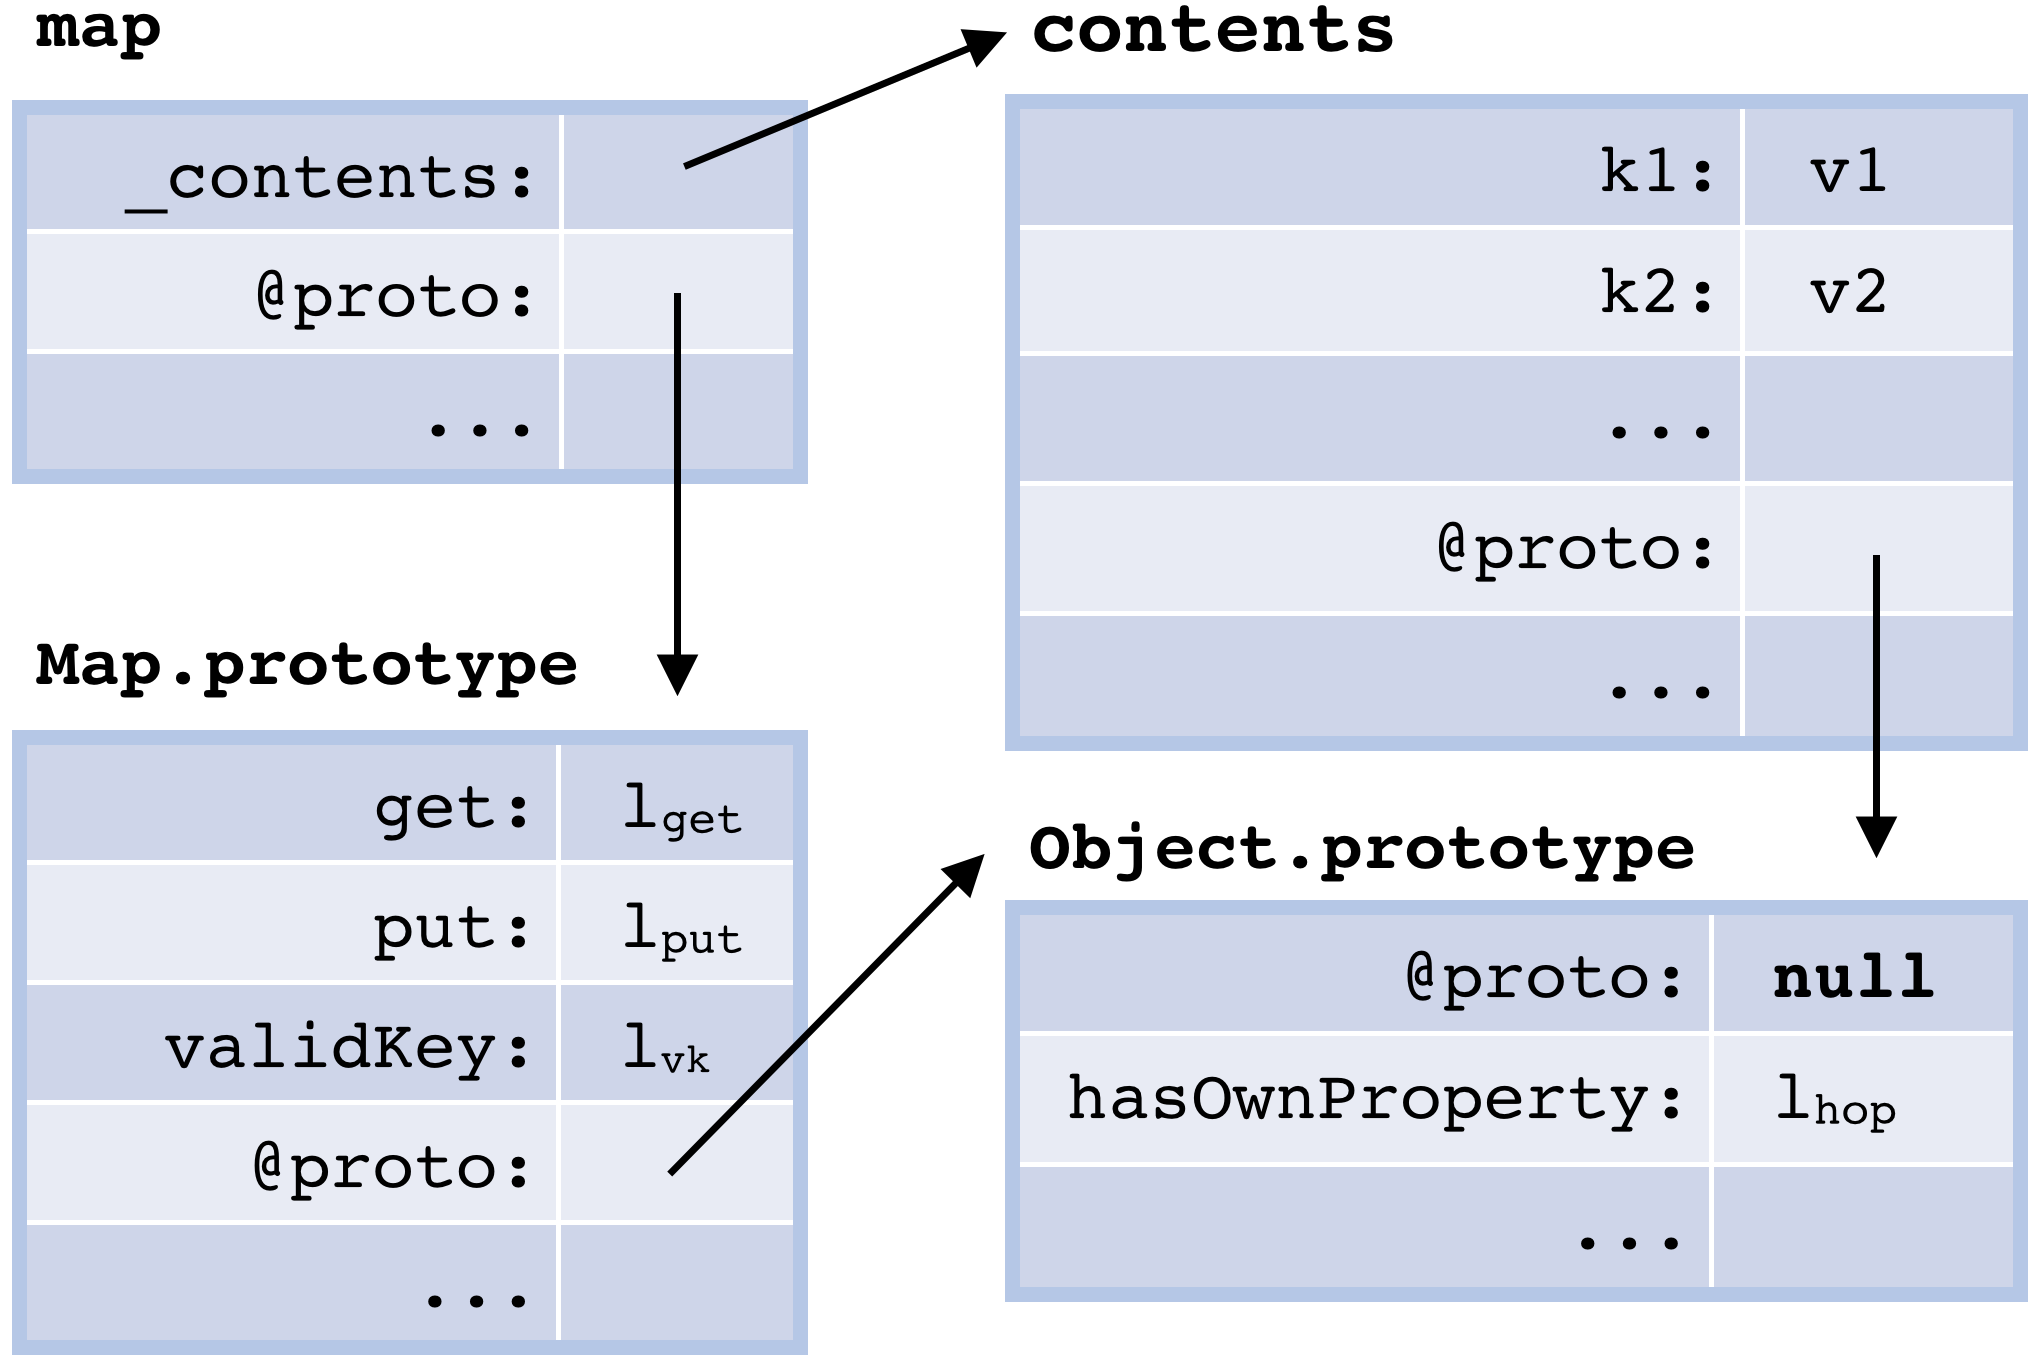
\includegraphics[width=0.93\textwidth]{figures/mapDiagram.png}
 \vspace*{0.5cm}
 \caption{General library heap}
 \label{fig:2b}
 \end{subfigure}
 %
 \begin{subfigure}[b]{0.3\textwidth}
 \centering 
 {\lstset{xleftmargin=.17\textwidth,language=JavaScript,basicstyle=\fontsize{7}{7}\ttfamily,escapeinside={~}{~}}
\begin{lstlisting}
var k = symb_string();
var v = symb_number();
assume(validKey(k));
var m = new Map(); m.put(k, v); 
var result = m.get(k);
assert(result = v)
\end{lstlisting}}
\vspace*{0.1cm}
 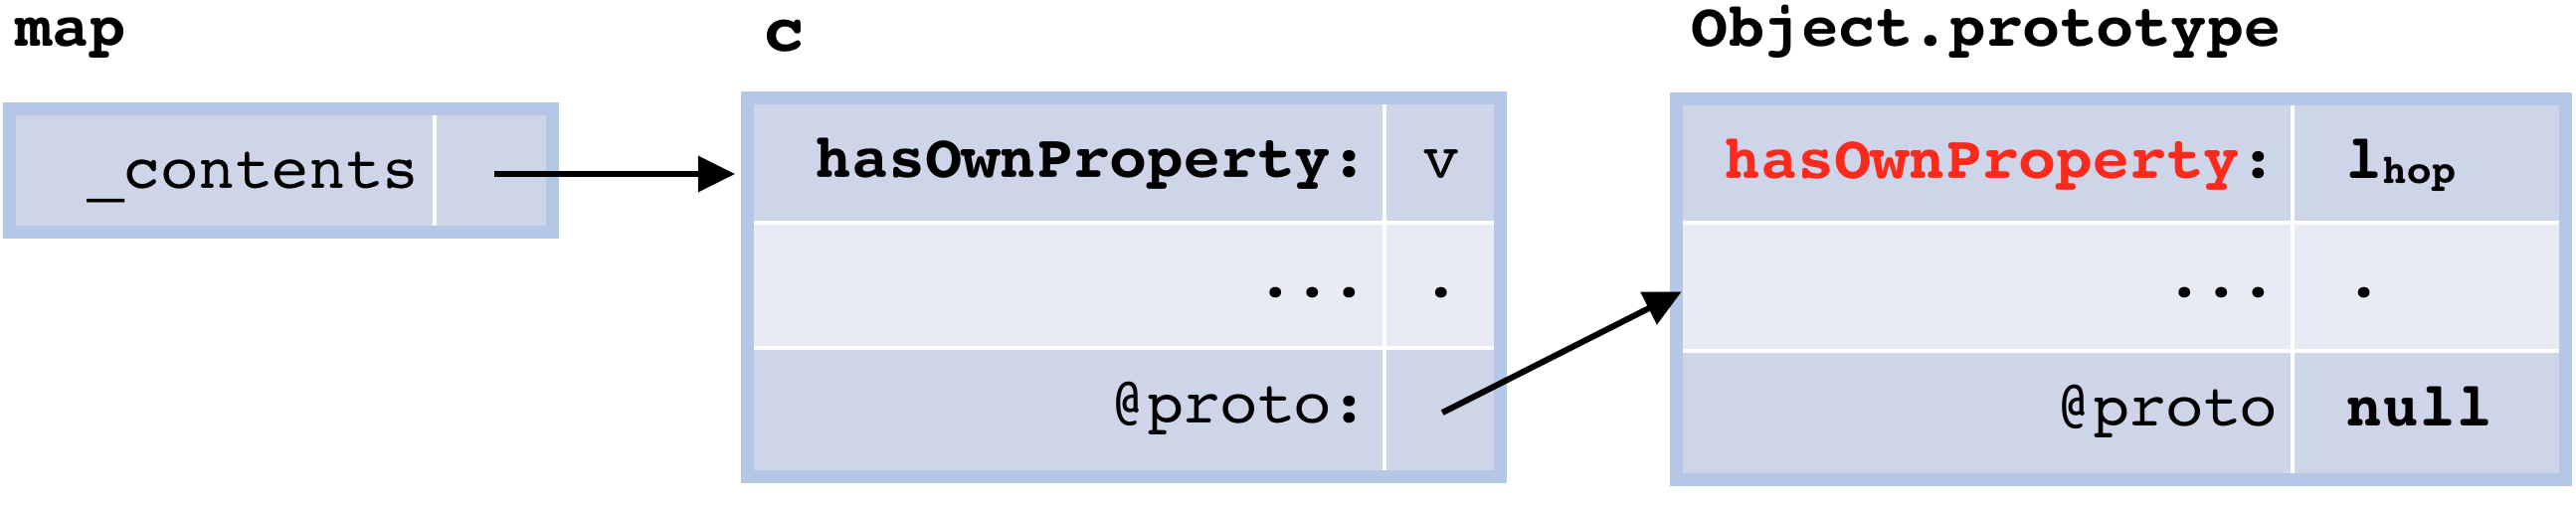
\includegraphics[width=0.78\textwidth]{figures/heapfail.png}
 \captionsetup{format=nastyCaption}
\caption{Simple symbolic test (above); \\the \jsinline|"hasOwnProperty"| bug (below)}
\label{fig:2c}
\end{subfigure}
\vspace*{-0.25cm}
\caption{Running example: JavaScript key-value map library}
\label{fig:two}
 \vspace*{-0.4cm}
\end{figure*}

Our running example is a \emph{key-value map} implementation, given in Figure~\ref{fig:2a}. It contains four functions: 
\jsinline|Map|, for constructing an empty map;
\jsinline|get|, for retrieving the value associated with a given key;
\jsinline|put|, for inserting/updating key-value pairs; and \jsinline|validKey|, for deciding whether or not a key is valid.
The map library implements a \emph{key-value map} as an object with property \jsinline|_contents|, denoting the object storing the map contents.  
The named properties of \jsinline|_contents| and their value attributes correspond to the map keys and values, respectively.
The functions \jsinline|get|, \jsinline|put|, and \jsinline|validKey| are shared between all map 
objects and are, therefore, defined in \jsinline|Map.prototype|, which is the prototype\footnote{In JavaScript, inheritance is modelled through \emph{prototype chains}. On property lookup, $\mathtt{o.p}$, we first check if the property $\mathtt{p}$ is present in the object $\mathtt{o}$, in which case its value is returned. Otherwise, we  check if $\mathtt{p}$ is present in the prototype of $\mathtt{o}$, and so  forth.} of all objects created using \jsinline|Map| as a constructor (i.e.,~using~\jsinline|new Map()|). 
The \jsinline|get| function returns the value associated with a given key in the map, or \jsinline|null| if the key is not in the map. 
Note that, in order to check that the given key is in the map, \jsinline|get| uses the built-in function \jsinline|hasOwnProperty|, which lives in \jsinline|Object.prototype|, the prototype of all objects.
The \jsinline|put| function updates the map if the supplied key is valid, and otherwise throws an error. 
The \jsinline|validKey| function describes the conditions under which a given key is valid. 

In Figure \ref{fig:2b}, we show a general heap of key-value maps. There is the \jsinline|map| object, with its \jsinline|_contents| property pointing to the \jsinline|contents| object and its prototype being \jsinline|Map.prototype|. There is the \jsinline|contents| object, which holds the key-value pairs, and whose prototype is \jsinline|Object.prototype|. There is the \jsinline|Map.prototype| object, which holds the \jsinline|get|, \jsinline|put|, and \jsinline|validKey| functions,\footnote{In JavaScript, functions are modelled as objects in the heap. As their structure does not add to this example, we only show the locations of the appropriate objects.} and whose prototype is also \jsinline|Object.prototype|. Finally, there is \jsinline|Object.prototype|, which holds the \jsinline|hasOwnProperty| function that is called by \jsinline|Map.prototype.get|.

%Observe that a naive implementation of the function \jsinline|validKey| may result in potential bugs. In particular, one can insert a key-value pair with \jsinline|"hasOwnProperty"| as a key into the map. By doing this, \jsinline|"hasOwnProperty"| in the prototype chain of \jsinline|_contents| is overridden and subsequent calls to \jsinline|get| will fail. 

%\myparagraph{Prototype chains and $\mathtt{Object.prototype}$}
%In order to better understand the implementation of the map library as well as its possible bugs, 
%one must first understand the \emph{prototype-based inheritance} mechanism of JavaScript. 
%Every JavaScript object has a prototype, which (for presentation purposes) we assume to 
%be stored  in an internal property \jsinline|@proto|. In order to determine the value of a property
%\jsinline|p| of an object \jsinline|o|, the semantics first checks if \jsinline|o| has a 
%property named \jsinline|p|, in which case the property look-up yields its value. Otherwise, the 
%semantics checks if \jsinline|p| belongs to the properties of the prototype of \jsinline|o| and so 
%forth. Hence, in the example, when looking up the value of the property \jsinline|hasOwnProperty|
%of the object \jsinline|contents|, one gets the value associated with the property  \jsinline|hasOwnProperty|
%of its prototype.
%The sequence of objects that can be accessed from a given object through the inspection 
%of the respective prototypes is called a \emph{prototype chain}.
%Prototype chains typically finish with the object \jsinline|Object.prototype| from which JavaScript 
%programs can access a number of built-in functions, which are part of the language runtime environment and are used for inspecting and manipulating objects.
%An example of such a function is \jsinline|hasOwnProperty(p)|, which checks whether or not the object 
%on which it is invoked has the property \jsinline|p| (e.g. {\small \jsinline|map.hasOwnProperty("_contents")|}
%evaluates to \jsinline|true| when evaluated in the heap shown in Fig.~\ref{map:example}-(right), 
%because the object \jsinline|map| has a property named~\jsinline|"_contents"|). 

\lstnewenvironment{lstjsex}{\lstset{language=JavaScript,basicstyle=\fontsize{8}{8}\ttfamily,escapeinside={~}{~}, numbers=none}}{}

\vspace*{-0.2cm}
\subsection{Whole-program Symbolic Testing}
\label{subsec:st}

Developers are used to writing unit tests for their code---verifying that, given some concrete inputs, the code produces the expected outputs. Using \cosette, they can write unit tests with \emph{symbolic} inputs and outputs, systematically testing a broad range of behaviours with a single symbolic test. For example, one meaningful unit test for the \jsinline|put| function consists of inserting a valid key-value pair \jsinline|(k, v)| into a map and then verifying that the pair has been inserted correctly. In Cosette, this test can be written as in Figure~\ref{fig:2c}. First, we declare \jsinline|k| to be a symbolic string and \jsinline|v| to be an symbolic number, using \cosette's constructs for creating symbolic variables. Next, we assume that \jsinline|k| is a valid key. Next, we create a new map, put the (symbolic) key-value pair \jsinline|(k, v)| into the map and then retrieve the value corresponding to the key~\jsinline|k|. Finally, we assert that the retrieved value is equal to the one we had previously put.

% 
When running \cosette on this test, if the \jsinline|validKey(k)| function was implemented incorrectly,\footnote{For instance, $\mathtt{validKey(k)}$ may only require that $\mathtt{k}$ is a string, which is a reasonable implementation, in the sense that it disallows JavaScript's implicit coercions.}
we will obtain the counter-model \jsinline|k = "hasOwnProperty"|. To understand this error, recall the heap and the implementation of \jsinline|get| from Figure~\ref{fig:two}. We can see that, if we were to put the key \jsinline|"hasOwnProperty"| into the contents object of a map, then the lookup of \jsinline|c.hasOwnProperty| done by \jsinline|get| will not reach \jsinline|Object.prototype| as intended, resolving instead to the \jsinline|hasOwnProperty| property of the \jsinline|contents| object (Figure~\ref{fig:2c}, below).

This example highlights how \cosette does not require specialist knowledge and can 
be used as a testing tool by a general JavaScript developer. The annotations amount to the creation of 
symbolic variables and the writing of assumptions and assertions, remaining minimal and intuitive, in contrast with the standard annotation burden of verification tools.

\vspace*{-0.2cm}
\subsection{Specification-driven Bug-finding}
\label{subsec:sdbf}

%\pmax{
%\begin{itemize}
%\item Compositionality = resilience to frame
%\item Summaries have to be resilient to frame
%\item BUT there are also NONES, and this is what is new
%\item Now guide through
%\item POINT - resilient to ALL frames, for whole-program analysis we are resilient only to one frame - we do get to create it, but it's only one after all
%\item Then, we can have more general specs, but needn't necessarily
%\end{itemize}
%}

As well as for whole-program analysis, \cosette can be used for compositional symbolic analysis of JavaScript functions in isolation, where the user specifies the functions in terms of their pre- and post-conditions. These specifications may account for only the parts of the heap required for running the function and can involve predicates, both recursive and non-recursive. We deal with recursive predicates by unfolding them to a  bound specified by the user.

Much like symbolic tests generalise concrete tests, specifications generalise symbolic tests. Given a JavaScript function, its specification, and the unfold depth for predicates, \cosette generates symbolic tests to verify that the function conforms to the specification up to that given depth. If this is not the case, \cosette will return a concrete counter-model that invalidates the specification. Unlike whole-program analysis tools, \cosette also tests if the given specification is compositional, that is, if it is resilient against all possible contexts in which the function can be run, and reports back to the user any found sources of non-compositionality.

\cosette supports the specification of symbolic states via simple separation logic assertions in the style of JaVerT~\cite{javert}. The developer has at their disposal a number of built-in predicates that capture the fundamental concepts of JavaScript (discussed throughout the text), and can define their own predicates as well. For instance, learning from the previous symbolic test, we could define the following predicate for describing valid keys:
\begin{Verbatim}[fontsize=\footnotesize,commandchars=\\\{\}]
    ValidKey(k) := types(k : Str) * (k <> "hasOwnProperty"),
\end{Verbatim}
\noindent meaning that \jsinline|k| is a valid key if it is a string that is not equal to \jsinline|"hasOwnProperty"|. From there, if we wanted to do a full functional correctness specification of the \jsinline|Map| library, we could, guided by the heap in Figure~\ref{fig:2b}, define the following two predicates:

% \textcolor{red}{(m, "get") -> None * (m, "put") -> None * (m, "validKey") -> None} * 
% * NoProps(c, keys)

\smallskip
\begin{Verbatim}[fontsize=\footnotesize,commandchars=\\\{\}]
 Map (m, mp, kvs) := JSObjectWithProto(m, mp) * 
   DataProp(m, "_contents", c) * JSObject(c) * KVPairs(c, kvs) * 
     \textcolor{red}{NoProp(m, "get")} * \textcolor{red}{NoProp(m, "put")} * \textcolor{red}{NoProp(m, "validKey")} * 
       \textcolor{blue}{NoProps(c, FProj(kvs))}
\end{Verbatim}
\begin{Verbatim}[fontsize=\footnotesize,commandchars=\\\{\}]
  KVPairs (c, kvs) := (kvs = \{ \}),
                      (kvs = \{(k, v)\} U kvs') * ValidKey(k) * 
                        DataProp(c, k, v) * KVPairs(c, kvs')
\end{Verbatim}

\smallskip
The \jsinline|Map| predicate states that a map object is a standard JavaScript object with a given prototype \jsinline|mp|, and that it has the property \jsinline|_contents|, which points to a  JavaScript object \jsinline|c|.
Using the \jsinline|KVPairs| predicate, % (explained shortly), 
it also states that \jsinline|c| holds the key-value pairs \jsinline|kvs|. 
%Finally, it obtains the set of keys \jsinline|keys| from the set of key-value pairs using the first projection predicate \jsinline|First|, and then, using the \jsinline|NoProps| predicate, states that all other properties are absent from \jsinline|c|.
The \jsinline|KVPairs(c, kvs)| predicate is defined recursively: \jsinline|kvs| is either empty or contains at least one key-value pair \jsinline|(k, v)|, 
in which case we state that the key \jsinline|k| must be valid, that object \jsinline|o| has  property \jsinline|k| with value \jsinline|v|, and proceed recursively.
The highlighted parts of \jsinline|Map| describe the compositionality requirements: in red, we state that map objects must not have the properties \jsinline|"get"|, \jsinline|"put"|, and \jsinline|"validKey"|; in blue, we state that the object~\jsinline|c| has no other properties except for the map keys.\footnote{$\mathtt{NoProp(o, p)}$  states that the object $\mathtt{o}$ does not have property $\mathtt{p}$; $\mathtt{NoProps(o, props)}$ states that the object $\mathtt{o}$ has no properties outside of those from the set $\mathtt{props}$; the $\mathtt{FProj}$ operator extracts the set of keys from the set of key-value pairs.}
%
%The uniqueness of keys is guaranteed by the \jsinline|DataProp| predicate of \jsinline|KVPairs| and the separating conjunction.
We also require a \jsinline|MapProto(mp)| predicate, describing that \jsinline|mp| is a valid map prototype, that is, that it defines the \jsinline|put|, \jsinline|get|, and \jsinline|validKey| methods. To avoid clutter, we keep its definition opaque.

\begin{wrapfigure}{R}{0.23\textwidth}
\vspace*{-0.3cm}
\hspace*{-0.8cm}
$
{\scriptsize
\begin{array}{c}
\left\{ {\begin{array}{c}
 \text{\texttt{Map(m, mp, kvs) * MapProto(mp) *}} \\
 \text{\texttt{ValidKey(k) * (k $\notin$ FProj(kvs)) *}} \\
 \text{\textcolor{blue}{\texttt{Writable(Object.prototype, k)}}}
\end{array}} \right\} \\
%
\text{\bfseries \texttt{m.put(k, v)}} \\[0.2mm]
%
\left\{ {\begin{array}{c}
 \text{\texttt{Map(m, kvs -u- (k, v)) * MapProto(mp) *}} \\
 \text{\textcolor{blue}{\texttt{Writable(Object.prototype, k)}}} \\
\end{array}} \right\}
\end{array}
} 
$
\vspace*{-0.4cm}
\end{wrapfigure}

On the right, we show one compositional specification of \jsinline|put(k, v)|. 
We assume a map object \jsinline|m|, with key-value pairs \jsinline|kvs| and prototype \jsinline|Map.Prototype|. We also assume that \jsinline|k| is a valid key not already in the map. For compositionality, highlighted in blue, we have to state that the property \jsinline|k| is not non-writable in \jsinline|Object.prototype|.\footnote{In JavaScript, object properties can be non-writable, meaning that their value cannot be changed. In this specification, we assume that the property exists and is writable. There is an analogous specification for $\mathtt{put}$, in which the property does not exist.}
In the end, the key-value pair has been inserted into the map, while the remaining part of the heap remains unchanged.

% for example, \jsinline|JSObject(o)| states that \jsinline|o| is a standard JavaScript object; \jsinline|JSObjectWithProto(o, op)| states that \jsinline|o| is a JavaScript object with prototype \jsinline|op|; and \jsinline|DataProp(o, p, v)| states that the property \jsinline|p| of~\jsinline|o| has value \jsinline|v|. One can also describe the absence of object properties: \jsinline|NoProp(o, p)| states that the object~\jsinline|o| does not have property \jsinline|p|, and \jsinline|NoProps(o, props)| states that the object \jsinline|o| has no other properties except those in the set \jsinline|props|. There also exist predicates for describing function objects, prototype chains, function closures, etc.,

%\smallskip
%\begin{minipage}{0.475\textwidth}
%\begin{displaymath} 
%{\scriptsize
%\begin{array}{c}
%\left\{ {\begin{array}{c}
% \text{\texttt{Map(m, mp, kvs -u- (k, v')) * MapProto(mp)}}
%\end{array}} \right\} \\
%%
%\text{\bfseries \texttt{m.put(k, v)}} \\[0.2mm]
%%
%\left\{ {\begin{array}{c}
% \text{\texttt{Map(m, kvs -u- (k, v)) * MapProto(mp)}}
%\end{array}} \right\}
%\end{array}
%} 
%\end{displaymath}
%\end{minipage}
%\quad
%\begin{minipage}{0.48\textwidth}
%%
%\begin{displaymath} 
%{\scriptsize
%\begin{array}{c}
%\left\{ {\begin{array}{c}
% \text{\texttt{Map(m, mp, kvs) * MapProto(mp) *}} \\
% \text{\texttt{ValidKey(k) * (k $\notin$ First(kvs))}}
%\end{array}} \right\} \\
%%
%\text{\bfseries \texttt{m.put(k, v)}} \\[0.2mm]
%%
%\left\{ {\begin{array}{c}
% \text{\texttt{Map(m, kvs -u- (k, v)) * MapProto(mp)}}
%\end{array}} \right\}
%\end{array}
%} 
%\end{displaymath}
%\end{minipage}

%\pmax{Explain specs a bit}

When symbolically testing the specifications of the \jsinline|Map| library functions, the \jsinline|"hasOwnProperty"| bug will not be triggered again, as \jsinline|ValidKey(k)| has been adjusted appropriately. However, if we were to forget the highlighted parts in the \jsinline|Map| definition and \jsinline|put| specification, we would encounter other issues, exposing the tension between compositionality and dynamic languages. 

\begin{wrapfigure}{R}{0.18\textwidth}
\vspace*{-0.4cm}
\hspace*{-0.6cm}
\centering
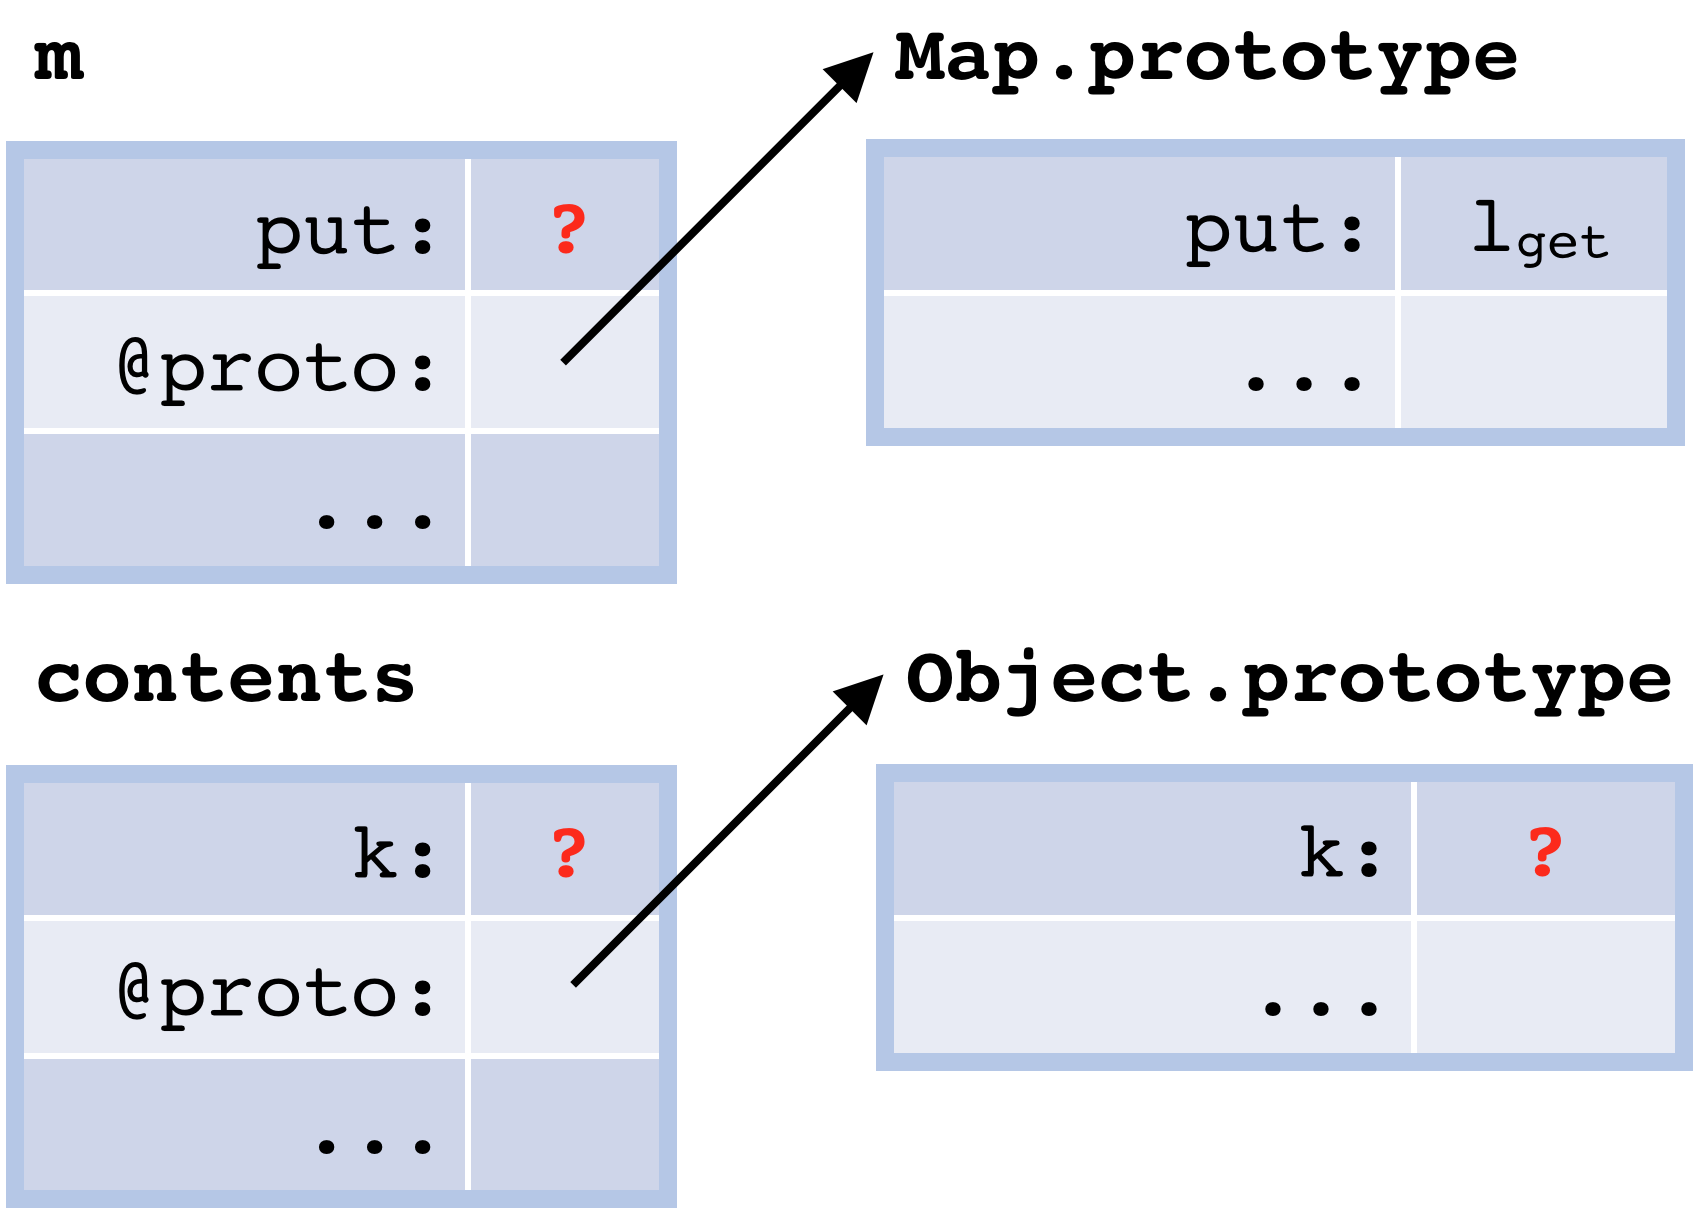
\includegraphics[width=0.21\textwidth]{figures/compositional.png}
\vspace*{-0.58cm}
\caption*{\hspace*{-0.58cm}{\small Figure 2. Compositionality}}
\vspace*{-0.4cm}
\end{wrapfigure}

\setcounter{figure}{2} 
First, if we omitted the part of the \jsinline|Map| predicate highlighted in red, \cosette would complain, when testing the \jsinline|put| function, that it has no information about the property \jsinline|"put"| of the map object~\jsinline|m| and cannot perform the lookup \jsinline|m.put| (Fig.~2, above). This means that the library code is not resilient to frames in which a map object \jsinline|m| has the property \jsinline|put|.
Analogous issues would arise for the \jsinline|"get"| and \jsinline|"validKey"| properties.% which also must be absent from all map objects. 

Second, if we omitted the parts highlighted in blue, upon execution of the line \jsinline|this._contents[k] = v| (Fig.~\ref{fig:2a}, line 12) \cosette would complain that it has no information about the property \jsinline|k| in the prototype chain of the contents object (Fig.~2, below). This is required as the semantics of JavaScript has to look up the value of the property \jsinline|k| of the contents object before performing the actual assignment, to check if the assignment is allowed (i.e.,~ that the property is non-writable). As \jsinline|k| is symbolic, what this means is that the library is not resilient to frames in which there are non-writable properties in \jsinline|Object.prototype|. A similar issue arises for the \jsinline|Map| constructor (Fig.~\ref{fig:2a}, line 1), which requires the property \jsinline|"_contents"| not to be non-writable in the prototype chains of map objects.

%Now, we can give the complete definition of the \jsinline|Map| predicate and the corrected, compositional specification of \jsinline|put(k, v)| when \jsinline|k| is a valid key that is not in the map, with the compositionality-related changes highlighted in red:
%
%\noindent
%\begin{minipage}{0.58\textwidth}
%\begin{Verbatim}[fontsize=\footnotesize,commandchars=\\\{\}]
%  Map (m, mp, kvs) := 
%    JSObjectWithProto(m, mp) * \textcolor{red}{NoProp(m, "get")} * 
%    \textcolor{red}{NoProp(m, "put")} * \textcolor{red}{NoProp(m, "validKey")} * 
%    DataProp(m, "_contents", c) * JSObject(c) *
%    KVPairs(c, kvs) * \textcolor{red}{First(kvs, keys)} * \textcolor{red}{NoProps(c, keys)}
%\end{Verbatim} 
%\end{minipage}
%\begin{minipage}{0.42\textwidth}
%%
%\begin{displaymath} 
%{\scriptsize
%\begin{array}{c}
%\left\{ {\begin{array}{c}
% \text{\texttt{Map(m, mp, kvs) * MapProto(mp) *}} \\
% \text{\texttt{ValidKey(k) * (k $\notin$ First(kvs)) *}} \\
% \text{\textcolor{red}{\texttt{Writable(Object.prototype, k)}}}
%\end{array}} \right\} \\
%%
%\text{\bfseries \texttt{m.put(k, v)}} \\[0.2mm]
%%
%\left\{ {\begin{array}{c}
% \text{\texttt{Map(m, kvs -u- (k, v)) * MapProto(mp) *}} \\
% \text{\textcolor{red}{\texttt{Writable(Object.prototype, k)}}} \\
%\end{array}} \right\}
%\end{array}
%} 
%\end{displaymath}
%\end{minipage}

What this example illustrates is that, in order to be compositional, specifications of programs written in dynamic languages have to explicitly state which parts of the heap must not be present. \cosette is able to detect and report compositionality-related issues, such as those presented above, which are highly likely to remain unnoticed in whole-program analysis, as there we always have complete information about the entire contents of the heap.

%\subsection{Compositional Symbolic Testing}
%
%%\begin{wrapfigure}{R}{0.45\textwidth}
%%\vspace*{-0.5cm}
%%\centering
%%\begin{lstjsex}
%%[ Map(m, mp) * MapProto(mp) * ValidKey(k) ]
%%    m.put(k, v); 
%%    var result = m.get(k);
%%[ Precondition * (result = v) ]
%%\end{lstjsex}
%%\vspace*{-0.4cm}
%%\caption{Revisited test for \jsinline|Map|}
%%\label{test:map:2}
%%\vspace*{-0.35cm}
%%\end{wrapfigure}
%
%A general developer can write concrete and symbolic tests for their code, but cannot be expected to write full functional correctness specifications in separation logic. Using \cosette, they can combine the best of both worlds by describing only the shape of their \polish{heap/memory/data structure} using separation logic and then testing the behaviour of the code using symbolic tests. Using this approach, one can not only find the same bugs as in whole-program symbolic testing, but also detect compositionality issues triggered by the tests. 



%Refer to Figure 2 - the developer knows the heap and can describe it easily. If they forget, . Ideally, this would be automatic.
%
%We illustrate the compositional symbolic execution of \cosette using the \jsinline|get(k)| function of the key-value map example. Below, we revisit the code of \jsinline|get| and describe the heap before and after \jsinline|get(k)| is called with a valid key that is in the map. In order to do this, the developer needs to know the structure of the heap (Figure~\ref{map:example}) and use the built-in predicates.
%
%\smallskip
%\begin{minipage}{0.52\textwidth}
% \begin{lstjs}
%Map.prototype.get = function (k) {
%  var c = this._contents;
%  if this.validKey(k) {
%    return (c.hasOwnProperty(k) ? 
%               c[k] : null)
%  } else throw new Error("Invalid Key");
%}
%\end{lstjs}
%\end{minipage}
%\begin{minipage}{0.47\textwidth}
%$
%{\scriptsize
%\begin{array}{c}
%\left\{{\begin{array}{c}
% \text{\texttt{JSObjectWithProto(this, mp) * MapProto(mp) * }} \\
% \text{\texttt{DataProp(m, "\_contents", c) * JSObject(c) * }} \\
% \text{\texttt{ValidKey(k) * \color{blue}{DataProp(c, k, v)}}}
%\end{array}}\right\} \\
%%
%\text{\bfseries \texttt{get(k)}} \\
%%
%\left\{ {\begin{array}{c}
% \text{\texttt{StartingState * (ret = v)}} 
%\end{array}} \right\}
%\end{array}
%}
%$
%\end{minipage}
%
%\smallskip
%To describe the starting state, we first note that the map object on which \jsinline|get| was called has prototype \jsinline|mp|, representing \jsinline|Map.prototype|.\footnote{Some stuff.} Next, we state that the map object itself has property \jsinline|"_contents"| pointing to a standard JavaScript object \jsinline|c|, that the key \jsinline|k| is valid, and that the object \jsinline|c| has the property \jsinline|k| with value \jsinline|v|. In the final state, we additionally know that the return value of the function should be equal to \jsinline|v|.
%
%
%
%
%
%\vspace*{5cm}
%catch how the spec is not compositional, reveal frame non-resilience shit
%
%It is meant to be run as a method call, the this, it is in the prototype. validKey is also meant to be in the prototype. Refer to figure 2. the this has the contents field, then that is an object, the key k is valid and then it may or may not have the k field.
%
%Now, frame bugs will pop up and you will see how the function is not resilient to the frame.
%
%you can catch these bugs in real-world tests
%
%...and if they want, they can write a more general abstraction of the entire data structure, which may be recursive or not, then ask for it to be unfolded to a given depth and create symbolic tests from that.
%
%
%
%\newpage
%In order for a specification of a program to be compositional, it must be resilient against all the possible frames, that is, all possible contexts in which the program can be run. This is in contrast to whole-program analysis, which considers only one frame at a time. 
%
%we demonstrate how \cosette explicitly exposes the resilience of JavaScript programs to the environment, not  considered by standard symbolic execution tools, but essential for compositional analysis. Therefore, this .
%
%For that, we revisit the \javert specification of key-value maps. This specification involves several predicates, shown below, which use JavaScript-specific abstractions that hide the internals of the language, such as \jsinline|JSObject(c)|, which states that \jsinline|c| is a standard JavaScript object, and \jsinline|DataProp(o, p, v)|, which states that the property \jsinline|p| of \jsinline|o| has value \jsinline|v|.
%
%% \textcolor{red}{(m, "get") -> None * (m, "put") -> None * (m, "validKey") -> None} * 
%
%\begin{Verbatim}[fontsize=\footnotesize,commandchars=\\\{\}]
%    Map (m, kvs) := DataProp(m, "_contents", c) * JSObject(c) * 
%                      KVPairs(c, kvs) * first(kvs, keys) * emptyFields(c, keys)
%\end{Verbatim}
% \begin{Verbatim}[fontsize=\footnotesize,commandchars=\\\{\}]
%KVPairs (o, kvs) := (kvs = \{ \}),
%                    (kvs = (k, v) -u- kvs') * ValidKey(k) * DataProp(o, k, v) * KVPairs(o, kvs')
%\end{Verbatim}
%\begin{Verbatim}[fontsize=\footnotesize,commandchars=\\\{\}]
%    ValidKey (k) := types(k : Str) * \textcolor{red}{(k <> "hasOwnProperty")}
%\end{Verbatim}
%
%
%Refer to Figure 2 - the developer knows the heap and can describe it easily. If they forget, . Ideally, this would be automatic.
%
%The \jsinline|Map| predicate captures the resource corresponding to a map object. 
%Concretely, it first states that the map object has the property \jsinline|_contents|, which points to a  JavaScript object \jsinline|c|.
%Next, using the \jsinline|KVPairs| predicate (explained shortly), it states that \jsinline|c| holds the key-value pairs \jsinline|kvs|. Finally, it obtains the set of keys \jsinline|keys| from the set of key-value pairs using the first projection predicate \jsinline|first|, and then, via the \jsinline|emptyFields| assertion, states that all other properties are absent from \jsinline|c|.
%
%The \jsinline|KVPairs(o, kvs)| predicate talks about key-value pairs of an object \jsinline|o|. 
%It is defined recursively on the structure of \jsinline|kvs| and it has two definitions, separated by a comma. 
%We have that \jsinline|kvs| is either empty or that it contains at least one key-value pair \jsinline|(k, v)|,\footnote{We write $\mathtt{-u-}$ for set union and omit the brackets around singleton sets.} 
%in which case we state that the key \jsinline|k| must be valid, that object \jsinline|o| has  property \jsinline|k| with value \jsinline|v|, and proceed recursively.
%The uniqueness of keys is guaranteed by the \jsinline|DataProp| predicate of \jsinline|KVPairs| and the separating conjunction.
%
%\begin{wrapfigure}{R}{0.3\textwidth}
%\vspace*{-0.45cm}
%\centering
%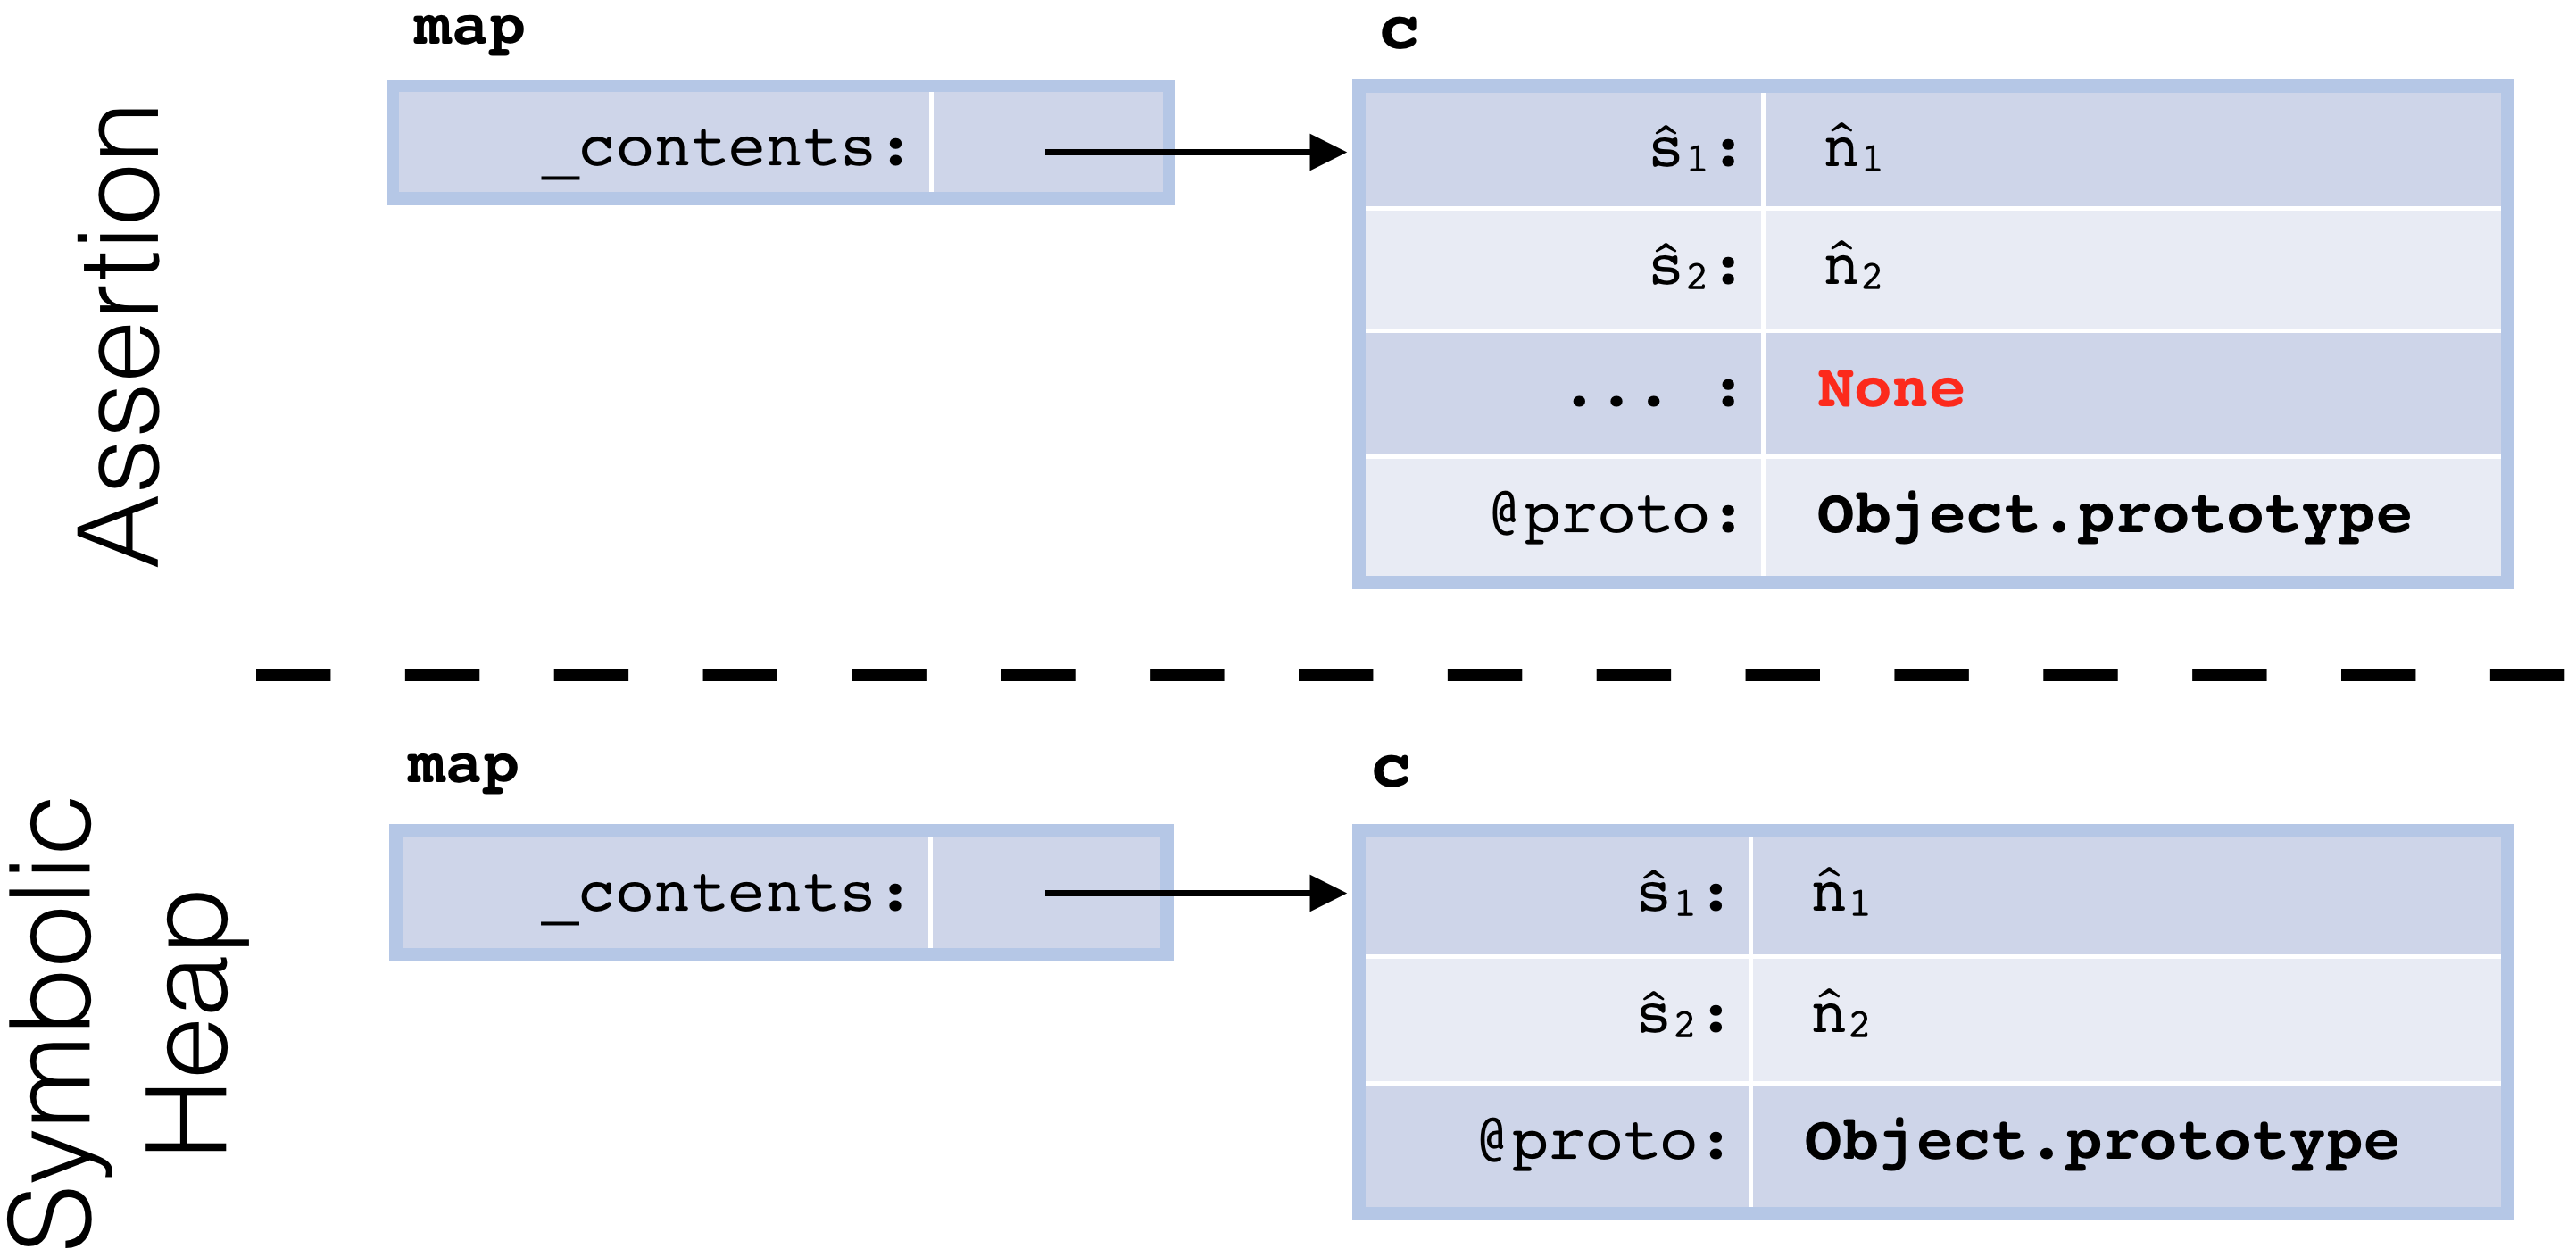
\includegraphics[width=0.29\textwidth]{figures/symbvsass.png}
%\vspace*{-0.3cm}
%\caption{Unfolded assertion {\scriptsize$\mathtt{Map(map, \{ (\hat{s}_1, \hat{n}_1), (\hat{s}_2, \hat{n}_2) \} )}$}}\label{fig:symb:state:versus:assertion}
%\label{fig:unfolded}
%\vspace*{-0.4cm}
%\end{wrapfigure}
%
%The \jsinline|ValidKey(k)| predicate captures the validity of a given key and holds \emph{iff} the corresponding JavaScript function \jsinline|validKey(k)| returns \jsinline|true|.
%In the definition of \jsinline|ValidKey|, we highlight in red a potential bug in the specification, already seen in the symbolic testing example.
%% source of errors on which we will focus shortly.
%
%To give a better intuition of how the \jsinline|Map| predicate works, we show the full unfolding of {\small$\mathtt{Map(map, \{ (k_1, v_1), (k_2, v_2) \} )}$} in Figure \ref{fig:symb:state:versus:assertion}. 
%
%\noindent
%\begin{minipage}{0.475\textwidth}
%\begin{displaymath} 
%{\scriptsize
%\hspace*{-0.2cm}
%\begin{array}{c}
%\left\{ {\begin{array}{c}
% \text{\texttt{Map(this, kvs -u- (k, v)) * ObjProtoF() *}} \\
% \text{\texttt{(this, "@proto") -> mp * MapProto(mp) * ...}}
%\end{array}} \right\} \\
%%
%\text{\bfseries \texttt{get(k)}} \\[0.2mm]
%%
%\left\{ {\begin{array}{c}
% \text{\texttt{Precondition * (ret = v)}} 
%\end{array}} \right\}
%\end{array}
%} 
%\end{displaymath}
%\end{minipage}
%\quad
%\begin{minipage}{0.48\textwidth}
%%
%\begin{displaymath} 
%{\scriptsize
%\begin{array}{c}
%\left\{ {\begin{array}{c}
% \text{\texttt{Map(this, kvs -u- (k, v')) * ObjProtoF() *}} \\
% \text{\texttt{(this, "@proto") -> mp * MapProto(mp) * ...}}
%\end{array}} \right\} \\
%%
%\text{\bfseries \texttt{put(k, v)}} \\[0.2mm]
%%
%\left\{ {\begin{array}{c}
% \text{\texttt{Map(this, kvs -u- (k, v)) * ObjProtoF() *}} \\
% \text{\texttt{(this, "@proto") -> mp * MapProto(mp) * ...}}
%\end{array}} \right\}
%\end{array}
%} 
%\end{displaymath}
%\end{minipage}
%
%\vspace{5pt}
%The predicate \jsinline|ObjProtoF()| describes the \jsinline|Object.prototype| object. It is needed because \jsinline|get| uses the \jsinline|hasOwnProperty| function, defined in \jsinline|Object.prototype|. 
%The predicate \jsinline|MapProto| specifies the resource of a valid map prototype: in particular, it defines the \jsinline|put|, \jsinline|get|, and \jsinline|validKey| methods.
%
%Given a JavaScript function, its separation logic specification, and the depth to which the unfold recursive predicates (non-recursive predicates are unfolded automatically), \cosette generates symbolic tests to verify that the function conforms to the specification up to that given depth.
%Now, if we forgot to state the part of the \jsinline|ValidKey(k)| predicate highlighted in red, that is, if we did not state that \jsinline|k <> "hasOwnProperty"|, the symbolic test generated for the specification of \jsinline|get| would fail for depth $\geq 1$, with the counter-model \jsinline|k = "hasOwnProperty"|, triggering the same bug previously described in the context of symbolic testing.

%\subsection{Catching \polish{procedure-local} bugs}
%
%The bug associated with the shadowing of the \jsinline|hasOwnProperty| property of \jsinline|Object.prototype| illustrates how a JavaScript library can be broken by only using its own functions. However, as JavaScript does not observe the frame property, there exists an additional class of bugs that can be triggered by the environment in which the library is run. These bugs expose how the library is not resilient against the possible frames and signal which properties of which objects must not be present in order for the library to behave correctly.
%
%To illustrate such bugs, recall the symbolic test from \S\ref{subsec:st}. This symbolic test creates an empty map on which it checks whether or not the behaviour of \jsinline|put| is correct. After catching the \jsinline|hasOwnProperty| bug, one might want to construct a more general test, starting from an arbitrary map. For this, one would need to use the \jsinline|Map| predicate from \S\ref{subsec:sdbf}:
%
%\begin{Verbatim}[fontsize=\footnotesize,commandchars=\\\{\}]
%         Map (m, kvs) := DataProp(m, "_contents", c) * JSObject(c) * 
%                           KVPairs(c, kvs) * first(kvs, keys) * emptyFields(c, keys)
%\end{Verbatim}
%
%\noindent as part of the initial state in which to run the symbolic test. Then, however, on execution of the test, when we reach the \jsinline|m.put(k, v)| command, we will get an error. The symbolic execution will not be able to determine if the property \jsinline|put|, which is supposed to be found in \jsinline|Map.prototype|, exists in the object~\jsinline|m| or not. This means that an environment can break the map library by putting into a map object the properties that are meant to be found in its prototype, and also that the specification of maps needs to be strengthened to forbid this explicitly:
%\begin{Verbatim}[fontsize=\footnotesize,commandchars=\\\{\}]
%   Map (m, kvs) := DataProp(m, "_contents", c) * JSObject(c) * 
%                     \textcolor{red}{((m, "get) -> none)} * \textcolor{red}{((m, "put") -> none)} * \textcolor{red}{((m, "validKey") -> none)} *
%                       KVPairs(c, kvs) * first(kvs, keys) * emptyFields(c, keys).
%\end{Verbatim}
%
%Bugs such as this will very rarely be caught by whole-program analyses, because there the entire state of the program is known and the test needs to be especially crafted with these bugs in mind. The reason that \cosette can catch them easily is because it is compositional and can run in partially described states.


\section{Extending Symbolic Execution with Separation Logic Assertions}
%!TEX root = ../main.tex
\subsection{\jsil Symbolic Execution with Separation Logic Assertions}
\label{subsec:sep:assertions}

We extend \jsil with a special construct, $\sepassert(P)$, for stating that 
the separation logic assertion $P$ must hold whenever $\sepassert(P)$ is evaluated. 
We use the assertion language of~\cite{javert}, with the following adaptation:
instead of \emph{untyped logical variables}, we 
use \emph{typed logical variables}, $\svar \in \svars$, which include 
symbolic numbers, $\snumber \in \snumbers$, strings $\sstring \in \sstrings$, 
and locations,~$\sloc \in \slocs$. 

\myparagraph{\jsil assertions: syntax and semantics}
\jsil assertions include: boolean operations; first-order connectives; the separating conjunction; 
existential quantification; and assertions for describing heaps. The $\lemp$ assertion describes 
an empty heap. The cell assertion, $(\lexpr_1,\lexpr_2) \pointsto \lexpr_3$,  describes an object 
at the location denoted by $\lexpr_1$ with a property denoted by $\lexpr_2$ that has the value 
denoted by $\lexpr_3$. The assertion $\emptyfields{\lexpr_1}{\lexpr_2}$ states that the object at 
the location denoted by $\lexpr_1$ has no properties other than possibly those included in the
set denoted by $\lexpr_2$. 
%
As in~\cite{gardner:popl:2012,javert}, in order to define the semantics of assertions, 
we resort to \emph{instrumented heaps} $\iheap \in \iheaps$, which differ from 
concrete heaps in that they may map object properties to the special value $\none$, 
explicitly indicating that the property does not exist (e.g. $\iheap(\loc, \jstring) = \none$
means that the object at location $\loc$ in the heap $\iheap$ does not have a property
named~$\jstring$). 
%Analogously, we extend symbolic heaps with $\none$-cells, obtained \emph{instrumented symbolic heaps} $\isheap \in \isheaps$. 
Instrumented heaps are related to heaps by means of an \emph{erasure 
function}, $\deabstract{.}: \iheaps \rightarrow \heaps$, %($\deabstract{.}: \isheaps \rightarrow \sheaps$), 
which simply removes the none-cells from the instrumented heap given as input.  Below, we give the syntax and semantics of \jsil assertions. Note that we assume pure assertions to have an empty spatial footprint and allow logical negation, conjunction, and disjunction of pure formulae only.

%  \deabstract{\jsilaheap}(\loc, x) = \jsilaheap(\loc, x) \iffdef (\loc, x) \in \domain(\jsilaheap) \ \wedge \ \jsilaheap(\loc, x) \neq \none

\begin{display}{\jsil Logic Assertions - Syntax and Semantics}
%
{\scriptsize \begin{tabular}{lll}
  %%%% 
  $\quad \lexpr \triangleq$ & $\lit \mid \jvar \mid \svar \mid \unoper\ \lexpr \mid \lexpr \binoper \lexpr$ &   \text{ Logical Expressions} \\[3pt]
  %%%%
  $\quad P_\pc\triangleq$ & $\jtrue \mid \jfalse \mid  \neg P_\pc \mid P_\pc \land P_\pc \mid P_\pc \lor P_\pc  \mid \lexpr = \lexpr \mid \lexpr \leq \lexpr$ & \text{~{Pure Assertions}} \\
  $\quad P\triangleq$ & $P_\pc \mid \lemp \mid (\lexpr, \lexpr)\pointsto \lexpr \mid \exists \svar. P \mid P \sep P  \mid \emptyfields{\lexpr}{\lexpr} $ &  \text{~Assertions} \\
\end{tabular}} \\ [5pt]
  %%%%%
  %%%%%
  
\quad 
{\scriptsize
\begin{tabular}{lll} 
       $\iheap, \store, \senv  \satisfies  \lemp$ & $\Leftrightarrow$ & $\iheap = \hemp$  \\[2pt]
           %
	   $\iheap, \store, \senv  \satisfies (\lexpr_1,\lexpr_2)\pointsto \lexpr_3$  &
            $\Leftrightarrow$ & $\iheap =  \hcell{\symbeval{\lexpr_1}{\store, \senv}}{\symbeval{\lexpr_2}{\store, \senv}}{\symbeval{\lexpr_3}{\store, \senv}}$  \\[2pt]
           % 
           $\iheap, \store, \senv  \satisfies P \sep Q$ & $\Leftrightarrow$ & $\exists \iheap_1, \iheap_2.  \, \iheap = \iheap_1 \dunion \iheap_2\ \wedge \ \iheap_1,  \store, \senv  \satisfies P \, \wedge \, \iheap_2,  \store, \senv \satisfies Q$ \\[2pt]
           %
           $\iheap, \store, \senv  \satisfies  \emptyfields{\lexpr_1}{\lexpr_2}$  &
                $\Leftrightarrow$ & $\iheap = \biguplus_{s \not\in \{ \symbeval{\lexpr_2}{\store, \senv} \}} ((\symbeval{\lexpr_1}{\store, \senv}, s) \pointsto \none)$
\end{tabular}}
\end{display}
%
For convenience, we define: 
\begin{align}
\sepmodels{P} = \left\{ (\heap, \store, \senv) \mid \exists \iheap \, . \,  \heap = \deabstract{\iheap} \ \wedge \ \iheap, \store, \senv \satisfies P  \right\}
\end{align}
Given a symbolic heap $\sheap$, a symbolic store $\sstore$, a path condition $\pc$, and 
an assertion $P$, we say that  $(\sheap, \sstore, \pc)$ \emph{satisfies} $P$, 
written $\sheap, \sstore, \pc \satisfies P$ \emph{if and only if}
$\smodels{\sheap, \sstore}{\pc} \subseteq \sepmodels{P}$. 
%
We can now give an \emph{ideal} symbolic semantics for the command $\sepassert(P)$ (which checks
if the current symbolic state satisfies $P$): 

\polish{the configurations need to be updated with the bot or top in the appropriate place. It appears 3 times: below, 
when the rules are re-stated with a call to the decision procedure, in Theorem 8.}
{\small \begin{mathpar}
\inferrule[\textsc{Assert - True}]
  { 
     \sheap, \sstore, \pc \satisfies P
  }{\symbtrans{\sheap, \sstore, \sepassert(P), \pc}{\sheap, \sstore, \pc}} 
\and
\inferrule[\textsc{Assert - False}]
  { 
          \sheap, \sstore, \pc \not\satisfies P
  }{\symbtranserr{\sheap, \sstore, \sepassert(P), \pc}{}{\pc}} 
\end{mathpar}}
\hspace{-3pt}Determining whether or not a symbolic state satisfies an SL-assertion $P$ is, in general, 
undecidable \cite{citemeplease}. Since we do not want to produce \emph{false positives}, in order to trigger 
an assertion failure, we need to find a concrete witness for that failure. More precisely, when executing 
$\sepassert(P)$ in the symbolic state $(\sheap, \sstore, \pc)$, the symbolic analysis must  
report an assertion failure only if it can find a concrete state $(\heap, \store)$  and a symbolic environment 
$\senv$ such that: 
$(\heap, \store, \senv) \in \smodels{\sheap, \sstore}{\pc}$ and
$(\heap, \store, \senv) \not\in \sepmodels{P}$.

%\begin{figure}[t!]
%\centering
%{\scriptsize
%\begin{mathpar} 
%\inferrule[\textsc{New Existential}]
%     { 
%         \svar \in \existentials 
%         \quad
%         \svar \not\in \domain(\subst)
%     }
%     {\unification{\sexpr, \pc}{\svar}{\subst}{\existentials} = \uyes{\subst[\svar \mapsto \sexpr]}}
%\quad
%\inferrule[\textsc{Matched Existential}]
%     { 
%         \subst(\svar) = \sexpr' 
%         \quad 
%         \pc \vdash \sexpr = \sexpr' 
%     }
%     {\unification{\sexpr, \pc}{\svar}{\subst}{\existentials} = \uyes{\subst}}
%\quad
%\inferrule[\textsc{Existential - None}]
%     { 
%         \subst(\svar) = \sexpr' 
%         \quad 
%         \pc \not\vdash \sexpr = \sexpr' 
%     }
%     {\unification{\sexpr, \pc}{\svar}{\subst}{\existentials} = \uno{\sexpr \neq \sexpr'}}
%\\
%\inferrule[\textsc{Grounded Expression}]
%     { 
%         \fv(\subst(\sexpr')) \cap \existentials = \emptyset
%         \quad 
%          \pc \vdash  \sexpr = \subst(\sexpr') 
%     }
%     {\unification{\sexpr, \pc}{\sexpr'}{\subst}{\existentials} = \uyes{\subst}}
%\qquad
%\inferrule[\textsc{Grounded Expression - Fail}]
%     { 
%         \fv(\subst(\sexpr')) \cap \existentials = \emptyset
%         \quad 
%          \pc  \not\vdash  \sexpr = \subst(\sexpr') 
%     }
%     {\unification{\sexpr, \pc}{\sexpr'}{\subst}{\existentials} = \uno{\sexpr  \neq \subst(\sexpr')}}
%%
%\\
%%
%\\
%\inferrule[\textsc{None-Cell Assertion}]
%	{  
%	   \subst(\symbeval{\lexpr_l}{\sstore})  = \loc 
%	   \quad 
%	    \symbeval{\lexpr_p}{\sstore} = \sexprp' 
%	   \quad
%       \sheap = \sheap' \dunion  \big((l, \sexprp_i) \mapsto \sexprv_i\big)\mid_{i = 0}^n    
%	   \quad
%	   (l, -) \not\in \domain(\sheap')  
%	   \quad
%	    \pc \vdash \sexprp' \not\in \{ \sexprp_i \mid_{i = 0}^n \} 
%	}{ \unification{\sheap, \sstore, \pc}{(\lexpr_l,\lexpr_p)\pointsto \none}{\subst}{\existentials} = \uyes{\subst, \sheap}} 
%%
%\\
%\inferrule[\textsc{None-Cell Assertion - Fail}]
%	{  
%	   \subst(\symbeval{\lexpr_l}{\sstore})  = \loc 
%	   \quad 
%	    \symbeval{\lexpr_p}{\sstore} = \sexprp' 
%	   \quad
%       \sheap = \sheap' \dunion  \big((l, \sexprp_i) \mapsto \sexprv_i\big)\mid_{i = 0}^n    
%	   \quad
%	   (l, -) \not\in \domain(\sheap')  
%	   \quad
%	    \pc \not\vdash \sexprp' \not\in \{ \sexprp_i \mid_{i = 0}^n \} 
%	}{ \unification{\sheap, \sstore, \pc}{(\lexpr_l,\lexpr_p)\pointsto \none}{\subst}{\existentials} = \uno{\sexprp' \in \{ \sexprp_i \mid_{i = 0}^n \} }} 
%%
%\\
%\inferrule[\textsc{EmptyFields Assertion}]
%	{  
%	  \loc = \subst(\symbeval{\lexpr_l}{\sstore}) 
%	   \quad 
%	     \symbeval{\lexpr_d}{\sstore} = \sexprv' 
%	   \quad
%	     \sheap = \sheap' \, \uplus \, \big((l, \sexprp_i) \mapsto \sexprv_i\big)\mid_{i = 0}^n   
%              \quad
%             (l, -) \not\in \domain(\sheap')
%	    \quad 
%	    \pc \vdash \big( \{ \sexprp_i \mid_{i = 0}^n   \} \subseteq \sexprv' \big)
%	}{ \unification{\sheap, \sstore, \pc}{\emptyfields{\lexpr_l}{\lexpr_d}}{\subst}{\existentials} = \uyes{(\subst, \sheap)}} 
%\\
%\inferrule[\textsc{EmptyFields Assertion - Fail}]
%	{  
%	   \loc = \subst(\symbeval{\lexpr_l}{\sstore}) 
%	   \quad 
%	     \symbeval{\lexpr_d}{\sstore} = \sexprv' 
%	   \quad
%	     \sheap = \sheap' \, \uplus \, \big((l, \sexprp_i) \mapsto \sexprv_i\big)\mid_{i = 0}^n   
%              \quad
%             (l, -) \not\in \domain(\sheap')
%	    \quad 
%	    \pc \not\vdash \big( \{ \sexprp_i \mid_{i = 0}^n   \} \subseteq \sexprv' \big)
%	}{ \unification{\sheap, \sstore, \pc}{\emptyfields{\lexpr_l}{\lexpr_d}}{\subst}{\existentials} = \uno{\{ \sexprp_i \mid_{i = 0}^n   \} \not\subseteq \sexprv'}} 
%\end{mathpar}
%\hrule
%\caption{Unification of spatial assertions:
% {\scriptsize$\unification{\sheap, \sstore, \pc}{\cell}{\subst}{\existentials} = \uyes{\subst', \sheap_f} \texttt{ OR } \uno{\pc'}$}}\label{fig:unification}}
%\end{figure}


\begin{table}
\centering
\renewcommand{\arraystretch}{1.2} 
{\scriptsize \begin{tabular}{@{}cccccccc@{}}\toprule
\multicolumn{3}{c}{{\it Symbolic State}} & &  & & & \\
\cmidrule{1-3}% \cmidrule{4-4}
\emph{Heap}  &  & \emph{PC}  &   &  \emph{Assertion}  & & \emph{Failing Constraint}       \\
\cmidrule{1-1} \cmidrule{3-3} \cmidrule{5-5}  \cmidrule{7-7}
%
$(\loc, \sexprp_1) \mapsto \sexprv$ & & $\jtrue$ & & 
	$(\loc, \sexprp_2) \mapsto \sexprv$ & &  $\sexprp_1 \neq \sexprp_2$ \\    
%
$(\loc, \sexprp_1) \mapsto \sexprv$ & & $\jtrue$ & & 
	$(\loc, \sexprp_1) \mapsto \sexprv \sep (\loc, \sexprp_2) \mapsto \none$ & &  $\sexprp_1 = \sexprp_2$ \\    
%
$(\loc, \sexprp_1) \mapsto \sexprv$ & & $\sexprp_1 \neq \sexprp_2$ & & 
	$(\loc, \sexprp_1) \mapsto \sexprv \sep (\loc, \sexprp_2) \mapsto \none \sep \emptyfields{\loc}{\{\sexprp_2, \sexprp_3\}}$ & &  $\sexprp_1 \neq \sexprp_3$ \\    
%
$(\loc, \sexprp_1) \mapsto \sexprv$ & & $\sexprp_1 \not\in \{\sexprp_2, \sexprp_3\}$ & & 
	$(\loc, \sexprp_1) \mapsto \sexprv \sep (\loc, \sexprp_2) \mapsto \none \sep (\loc, \sexprp_3) \mapsto \none$ & &  $\sexprp_2 = \sexprp_3$ \\    

\bottomrule
\end{tabular}}
\vspace{2pt}
\caption{Symbolic States vs Assertions\label{example:symb:states:vs:assertions}}
\vspace*{-0.7cm}
\end{table}

\subsection{Finding Counter Models for SL Assertions}
\label{subsec:countermodels}

We describe a partial decision procedure, which we  
implement as part of the \jsil symbolic interpreter, for proving entailments 
between symbolic states and SL-assertions \underline{and} finding counter 
models in case of failure.  
% I have to give more examples
As it is customary~\cite{javert,jacobs2011verifast,sepwithsmt}, the decision procedure works by first using \emph{pattern-matching} 
on the spatial part of the SL-assertion, and then discharging the pure part of the 
entailment to an external constraint solver (in our case, \rosette). 

\myparagraph{Representation of SL-assertions}
We target SL-assertions $P$ that can be represented as quadruples,
$(\existentials, \cells, \efs, \pfs)$, consisting of: 
\dtag{1} a set $\existentials$ of existentially quantified symbolic locations, 
\dtag{2} a list $\cells$ containing the non-none cell assertions (those whose value is different from $\none$), 
\dtag{3} a set $\efs$ containing the none-cell assertions and the empty-fields assertions, and
\dtag{4} a pure assertion $\pfs$. 
Hence, letting $\existentials = \{ \sloc_1, ..., \sloc_k \}$, $\cells = [ \cell_i \mid_{i = 0}^n ]$, and
$\efs = \{\efa_i \mid_{i = 0}^m \}$, we write $P \equiv (\existentials, \cells, \efs, \pfs)$ as shorthand for: 
 \begin{equation}
P = \exists \sloc_1, ..., \sloc_k \, . \big( \bigoast_{0 \leq i \leq n} \cell_i \ \sep  \bigoast_{0 \leq i \leq m} \efa_i \big) \ \lstar \ \pfs
\end{equation}
Given a symbolic state $(\sheap, \sstore, \pc)$ and an assertion $P \equiv (\existentials, \cells, \efs, \pfs)$, 
we represent each possible mapping from the existentially quantified symbolic locations in $P$ 
to the concrete locations in $\sheap$ as a \emph{substitution function} $\subst : \slocs \rightharpoonup \locs$.
Since both $\existentials$ and the set of concrete locations in $\sheap$ 
are finite, we conclude that there is a finite number of substitution functions to be considered 
when checking if $(\sheap, \sstore, \pc)$ satisfies $P$. 
Hence, in the following, we will assume a fixed substitution,~$\subst$. %\polish{Does this paragraph need to be rewritten? Stores?}
Furthermore, we assume that the SL-assertion given as input to the decision procedure does not contain any program variables. This we justify by noting that the following equivalence holds (the proof can be found in the Appendix):  
\begin{equation}
 \sheap, \sstore, \pc \satisfies P \iff \sheap, \emptystore, \pc \satisfies \symbeval{P}{\sstore},
\end{equation}
where $\symbeval{P}{\sstore}$ denotes the SL-assertion obtained by symbolically evaluating 
all the symbolic expressions in $P$ under $\sstore$.
%To obtain an SL-assertion in the targeted format, it suffices to symbolically evaluate all its symbolic expressions under the appropriate symbolic store. 



\begin{figure}[!t]
{\scriptsize
\begin{mathpar} 
\inferrule[\textsc{Cell Assertion}]
	{  
	    \sheap = \sheap_f \dunion ((l, \sexprp') \mapsto \sexprv') 
	   \\\\
	    \pc \vdash  \sexprp = \sexprp' \wedge \sexprv = \sexprv'
	}{\cellunification{\sheap, ((\loc,\sexprp)\pointsto \sexprv) \lstcons \cells}{\sheap_f, \cells}{\pc}} 
\and
\inferrule[\textsc{Cell Assertion - Fail}]
	{  
	   \sheap = \sheap' \dunion  \big((l, \sexprp_i) \mapsto \sexprv_i\big)\mid_{i = 0}^n  
	   \quad 
	     l \notin \hlocs{\sheap'}
	    \\\\ 
	     \pc_i = (\sexprp_i = \sexprp' \wedge \sexprv_i = \sexprv')\!\mid_{i = 0}^n
	    \quad
	    \pc \not\vdash \pc_i \mid_{i = 0}^n
	}{  \cellunificationx{\sheap, ((\loc,\sexprp)\pointsto \sexprv) \lstcons \cells}{\uno{\wedge_{0 \leq i \leq n} \neg\pc_i}}\pc } 
\end{mathpar}}
\vspace*{-0.5cm}
\caption{Unification of non-none cells: $\cellunification{\sheap, \cells}{\sheap_f, \cells'}{\pc}$
and $\cellunificationx{\sheap, \cells}{\uno{\pc'}}{\pc}$}
%$\unification{\sheap, \pc}{\cell}{} = \uyes{\sheap_f} \texttt{ or } \uno{\pc'}$}
\label{fig:uninonnone}
\vspace*{-0.2cm}
\end{figure}


\myparagraph{Unification rules}
In Figure \ref{fig:uninonnone}, we show the unification rules for non-none cell assertions. 
We write $\cellunificationx{\sheap, \cell \lstcons \cells}{-}\pc$ to denote the unification of a symbolic heap $\sheap$ against a single non-none cell $\cell$, given a path condition $\pc$.\footnote{We denote the transitive closure of $\rightarrow_{\mathcal{CU}}$ by $\rightarrow_{\mathcal{CU}}^*$.}  This unification can either terminate
successfully, with $\tuple{\sheap_f, \cells}$, in which case $\sheap_f$ denotes the
symbolic heap %to be framed off
that \underline{does not} contain the footprint of $\cell$, 
 and $\cells$ denotes the list of remaining non-none cell assertions to be unified (\textsc{Cell Assertion}); or unsuccessfully, with $\uno{\pc'}$, 
in which case $\pc'$ captures the constraints required for the unification to provably fail (\textsc{Cell Assertion - Fail}).
For instance, in the first example of Table~\ref{example:symb:states:vs:assertions}, 
in order to generate a witness for the entailment failure, we need to instantiate $\sexprp_1$ and $\sexprp_2$ so that the \emph{failing constraint} $\sexprp_1 \neq \sexprp_2$ is satisfied. 

%Given a cell assertion $\cell$, a symbolic state $(\sheap, \pc)$, 
%and a substitution $\subst$: 
%\begin{itemize}
%    \item if $\unification{\sheap, \pc}{\cell}{} = \uyes{\sheap_f}$, then there are 
%            two heaps $\sheap'$ and $\sheap_f$, such that $\sheap = \sheap' \dunion \sheap_f$
%            and $\smodels{\sheap', -}{\pc} \subseteq \sepmodels{\cell}$; 
%   
%   \item if $\unification{\sheap, \pc}{\cell}{} = \uno{\pc'}$, then there are 
%            no two heaps $\sheap'$ and $\sheap_f$, such that $\sheap = \sheap' \dunion \sheap_f$ 
%            and $\smodels{\sheap', -}{\pc \, \wedge \, \pc'} \subseteq \sepmodels{\cell}$.
%\end{itemize}

%\vspace{-3pt}
%\begin{display}{Unification of negative-resource assertions: $\unificationef{\sheap}{\efs} = \pc$ and $\sanity{\efs} = \pc$}

Unification of negative resource, that is, none-cells and \jsinline|emptyFields| assertions, is more intricate, as symbolic heaps do not maintain negative information. We denote by $\unificationef{\sheap}{\efs}$ the constraints that need to be satisfied for the unification of a symbolic heap $\sheap$ against the negative resource denoted by $\efs$ to succeed, and show the rules in Figure \ref{fig:unineg}. First, unifying a symbolic heap $\sheap$ that contains the object $\loc$ with properties $\sexprp_i|_{i=0}^n$ against a none-cell $(\loc,\sexprp)\pointsto \none$ effectively means that $\sexprp$ has to be different from all $\sexprp_i|_{i=0}^n$ (\textsc{NR-None Cell}). Next, unifying a symbolic heap $\sheap$ that contains the object $\loc$ with properties $\sexprp_i|_{i=0}^n$ against an  \jsinline|emptyFields| assertion $\emptyfields{\loc}{\sexpr_d}$ means that all of the properties $\sexprp_i|_{i=0}^n$  have to be in the domain of of the \jsinline|emptyFields| assertion, $\sexpr_d$ (\textsc{NR-Empty Fields}). 
The second and third examples of Table~\ref{example:symb:states:vs:assertions} illustrate unification failures resulting from NR-constraints not being satisfied: the second example targets the (\textsc{NR-None Cell}) rule, with the failing constraint: $\sexprp_1 \neq \sexprp_2$; and the third example targets the (\textsc{NR-Empty Fields}) rule, with the failing constraint $\sexprp_1 \not\in \jsilset{\sexprp_2, \sexprp_3}$.

\begin{figure}[!t]
{\scriptsize
\begin{mathpar} 
\inferrule[\textsc{NR-None Cell}]
	{  
	   \sheap = \sheap' \, \uplus \, \big((l, \sexprp_i) \mapsto -\big)\mid_{i = 0}^n   
	   \\\\
	    l \notin \hlocs{\sheap'}
	    \quad 
	    \pc = \wedge_{0 \leq i \leq n} \sexprp \neq \sexprp_i 
	 }{ \unificationefl{\sheap}{(\loc,\sexprp)\pointsto \none} =  \pc  }
\qquad
\inferrule[\textsc{NR-Empty Fields}]
	{  
	    \sheap = \sheap' \dunion  \big((l, \sexprp_i) \mapsto -\big)\mid_{i = 0}^n   
	    \\\\
	     l \notin \hlocs{\sheap'}
	     \quad 
	    \pc = \{ \sexprp_i \mid_{i = 0}^n \} \subseteq \sexpr_d 
	}{ \unificationefl{\sheap}{\emptyfields{\loc}{\sexpr_d}}{} =  \pc  } 
%
\\

\inferrule[\textsc{NR-Unification}]
	{}{ \unificationef{\sheap}{\efs} =  \bigwedge_{\efa \in \efs}  \unificationefl{\sheap}{\efa}} 
\\
\inferrule[\textsc{Separation Constraints - Fixed Location}]
	{
		 \efproj{\efs}{\loc} = \emptyfields{\loc}{\sexpr_d} \sep  \oast_{i = 0}^{n} \, \big((l, \sexprp_i) \mapsto \none \big)
	}{ \sanityl{\efs}{\loc} = 
		 (\wedge_{0 \leq i, j \leq n, i \neq j} \sexprp_i \neq \sexprp_j)
		       \, \wedge \,  ( \wedge_{0 \leq i \leq n} \sexprp_i \in \sexpr_d )
	} 
\and
\inferrule[\textsc{Separation Constraints}]
	{}{ \sanity{\efs} = \bigwedge_{\loc \in \eflocs(\efs)}\sanityl{\efs}{\loc}} 
\end{mathpar}}
\vspace*{-0.6cm}
\caption{Unification of negative-resource assertions: $\unificationef{\sheap}{\efs} = \pc$ and $\sanity{\efs} = \pc$}
\label{fig:unineg}
\vspace*{-0.2cm}
\end{figure}

Furthermore, due to the semantics of the separating conjunction, there are additional  constraints imposed by the negative resource. Concretely, all none-cells for the same object have to have different property names, and if any none-cell is starred together with an \jsinline|emptyFields| assertion for the same object, then its property name has to be in the domain of that \jsinline|emptyFields| assertion (\textsc{Separation-Constraints - Fixed Location}). 
We call these constrants \emph{separation constraints}, and denote them, for a fixed location~$\loc$, by $\sanityl{\efs}{\loc}$ in Figure~\ref{fig:unineg}. The point is that, if a given symbolic state entails a negative resource assertion, it must be the case that its path condition entails the corresponding separation constraints.
The last example of Table~\ref{example:symb:states:vs:assertions} illustrates a unification failure resulting from an EF-separation-constraint not being satisfied,
namely $\sexprp_2 \neq \sexprp_3$. 

Finally, the (\textsc{NR-Unification}) and (\textsc{Separation Constraints}) rules extend $\unificationef{\sheap}{\efs}$ and $\sanityl{\efs}{\loc}$, respectively, to sets of negative resource formulas.

\begin{figure}[t!]
{\scriptsize
\centering
\begin{mathpar} 
\inferrule[\textsc{Fail - Cell Unification}]
	{  
	   \cellunificationiterx{\sheap, \cells}{\uno{\pc''}}{\pc}
	}{\unificationfullfail{\sheap, \pc}{\cells, \efs, \pfs'}{}{\pc''}} 
\and
\inferrule[\textsc{Fail - Extra Resource}]
	{  
	     \cellunificationiter{\sheap, \cells}{\sheap_f, []}{\pc}
	     \qquad
	     \sheap_f \neq \hemp
	}{\unificationfullfail{\sheap, \pc}{\emptyset, \efs, \pfs'}{}{\jtrue}} 
\\
%
%
\inferrule[\textsc{Fail - Pure Entailment}]
	{  
	   \cellunificationiter{\sheap, \cells}{\hemp, []}{\pc}
	   \\\\
	   \pc'' = \unificationef{\sheap}{\efs} \wedge \, \sanity{\efs}
	   \quad
             \pc \not\vdash \pfs' \, \wedge \, \pc''
	}{\unificationfullfail{\sheap, \pc}{\cells, \efs, \pfs'}{}{\neg(\pc'  \, \wedge \, \pc'')}} 
\and
\inferrule[\textsc{Success}]
	{     
	   \cellunificationiter{\sheap, \cells}{\hemp, []}{\pc}
	   \\\\
	   \pc \vdash \pfs' \, \wedge \, \unificationef{\sheap}{\efs}   \, \wedge \, \sanity{\efs}
	}{\unificationfull{\sheap, \pc}{\cells, \efs, \pfs'}{}} 
%
\end{mathpar}}
\vspace*{-0.6cm}
\caption{Unification algorithm: {\small $\unificationfull{\sheap, \pc}{\cells, \efs, \pfs'}{}$}
and {\small $\unificationfullfail{\sheap, \pc}{\cells, \efs, \pfs'}{}{\pc'}$}.\label{unification:algorithm}}
\vspace*{-0.3cm}
\end{figure}

%\pmax{Stopped here.}

\myparagraph{Unification Algorithm}
Figure~\ref{unification:algorithm} presents the rules for the \emph{unification algorithm}. 
We write $\unificationfull{\sheap, \pc}{\cells, \efs \pfs'}{}$ to mean that the unification of 
the symbolic state $\sheap, \pc$ against the assertion $P \equiv (\emptyset, \cells, \efs, \pfs')$ 
succeeds, and $\unificationfullfail{\sheap, \pc}{\cells, \efs, \pfs'}{}{\pc'}$ to mean that it
fails, with the \emph{failing constraints} being: $\pc'$. Note that in order to generate a 
witness for the unification failure, one needs to find a symbolic environment satisfying the 
failing constraints.

The algorithm works by trying to unify the non-none cell assertions first. 
The unification succeeds when they are all successfully unified, the resulting symbolic heap is empty, 
and the final pure entailment is discharged by the constraint solver (\textsc{Success}). 
On the other hand, the unification can fail in three
ways: 
a non-none cell may not be unifiable (\textsc{Fail - Cell Unification}); 
all non-none cells are unifiable, but there may be additional resource left (\textsc{Fail - Extra Resource}); 
and all non-none cells are unifiable, there is no additional resource left, but the final
pure entailment may not be discharged by the constraint solver (\textsc{Fail - Pure Entailment}). 
Note that in case of failure, the algorithm 
always returns the constraints that need to be satisfied for a witness of that failure to be produced. 

Below we present the rules of the unification algorithm for a general assertion $P$.
For clarity, we use $\substs(\existentials, \sheap)$ to denote the set of all substitutions
mapping symbolic location in $\existentials$ to concrete locations in the domain of $\sheap$. 
%
For the success case, we simply need to find a substitution $\subst$ 
for which the unification algorithm terminates successfully. For the failure case, 
we need to compute the failing constraints for all possible substitutions, and 
return their conjunction. 


\begin{display}{Unification of General Assertions}
%\centering
 \inferrule[\textsc{Failure}]
 { 
     P \equiv (\existentials, -, -, -) 
     %
     \qquad
     %
     \substs(\existentials, \sheap) = \{ \subst_1, ..., \subst_n \}
    \\\\
     \forall_{1 \leq k \leq n}  . \, \big( \symbeval{\subst(P)}{\sstore} \equiv (\emptyset, \cells, \efs, \pfs') 
           \, \wedge \,  \unificationfullfail{\sheap, \pc}{\cells, \efs, \pfs'}{}{\pc_k}  \big)
     %
 }{\unificationfullfailP{\sheap, \sstore, \pc}{P}{\wedge_{0 \leq k \leq n} \pc_k}}
 
 \\
 
 \inferrule[\textsc{Success}]
 { 
    \exists \subst . \, \symbeval{\subst(P)}{\sstore} \equiv (\emptyset, \cells, \efs, \pfs')
    \\\\ \unificationfull{\sheap, \pc}{\cells, \efs, \pfs'}{}
 }{\unificationfullP{\sheap, \sstore, \pc}{P}{}}

 \end{display}

We can now give the \emph{implemented} symbolic semantics for the command $\sepassert(P)$ 
which makes use of the unification algorithm described above: 
{\small \begin{mathpar}
\inferrule[\textsc{Assert - True}]
  { 
      \unificationfullP{\sheap, \sstore, \pc}{P}{}
  }{\symbtrans{\sheap, \sstore, \sepassert(P), \pc}{\sheap, \sstore, \pc}} 
\and
\inferrule[\textsc{Assert - False}]
  {  
       \unificationfullfailP{\sheap, \sstore, \pc}{P}{\pc'}  
      \qquad
      (\pc \, \wedge \, \pc') \text{ is satisfiable}  
  }{\symbtranserr{\sheap, \sstore, \sepassert(P), \pc}{}{\pc \, \wedge \, \pc'}} 
\end{mathpar}}


\myparagraph{Soundness}
Theorem \ref{teo:unification:soundness} states that the unification algorithm is sound: given an SL-assertion~$P$ and a 
symbolic state $(\sheap, \sstore, \pc)$, if $\unificationfullP{\sheap, \sstore, \pc}{P}{}$ then the symbolic state
$(\sheap, \sstore, \pc)$ satisfies~$P$. 
The bug-finding theorem, Theorem \ref{teo:bugfinding}, is more subtle. It states that, in case of failure,  to find a counter-model 
for $P$, one has to pick a concretisation of the symbolic state that is consistent with 
the failing constraint generated by the unification algorithm. 



\begin{theorem}[Soundness of Unification]\label{teo:unification:soundness}
$\forall P, \sheap, \sstore, \pc \, .$
$$
\begin{array}{l}
   \unificationfullP{\sheap, \sstore, \pc}{P}{}
    \implies \smodels{\sheap, \sstore}{\pc} \subseteq \sepmodels{P}   
\end{array}
$$ 
\end{theorem}


\begin{theorem}[Bug-finding for SL]\label{teo:bugfinding}
$\forall P, \sheap, \sstore, \pc.$
$$
\unificationfullfailP{\sheap, \sstore, \pc}{P}{\pc'} \implies 
   \smodels{\sheap, \sstore}{\pc \wedge \pc'} \cap \sepmodels{P} = \emptyset
$$ 
\end{theorem}
%
The {\bf proofs} of the above results are given in the Appendix.

%\begin{theorem}[Soundness of Unification]\label{teo:unification:soundness}
%$\forall P, \cells, \efs, \pfs',  \sheap, \sstore, \pc, \subst \, .$
%$$
%\begin{array}{l}
%\symbeval{\subst(P)}{\sstore} \equiv (\emptyset, \cells, \efs, \pfs')\implies\unificationfull{\sheap, \pc}{\cells, \efs, \pfs'}{} \
%    \implies \smodels{\sheap, \sstore}{\pc} \subseteq \sepmodels{P}   
%\end{array}
%$$ 
%\end{theorem}
%
%
%\begin{theorem}[Bug-finding for SL]\label{teo:bugfinding}
%$\forall P, \existentials, \sheap, \sstore, \pc, \pc'.$
%$$
%\begin{array}{l}
%   P \equiv (\existentials, -, -, -) \implies \\
%   \quad \big( \forall \subst, \cells, \efs, \pfs''.\ \subst \in \substs(\existentials, \sheap) \implies 
%   \symbeval{\subst(P)}{\sstore} \equiv (\emptyset, \cells, \efs, \pfs'') \implies \\
%   \qquad \unificationfullfail{\sheap, \pc}{\cells, \efs, \pfs''}{}{\pc'''} \ \wedge \  \pc' \vdash \pfs''' \big) \implies \\
%   \qquad \quad \smodels{\sheap, \sstore}{\pc \wedge \pc'} \cap \sepmodels{P} = \emptyset.   
%\end{array}
%$$ 
%\end{theorem}



\subsection{Compiling \jsil Logic Specifications to Symbolic Tests}
\label{specs:to:symbolic:tests}

\begin{figure*}
\begin{center}
$$
\begin{array}{ll}
\testify{\fnormal}(\fid, \svar_i\mid_{i=0}^n, \pc, Q) \ \semeq & \\
         \dspc \dspc  \darkmath{\sf proc} \jsilmain () \{ 
         &  \text{Generated testing procedure for \underline{normal}-return specification:} \\ 
             \dspc \dspc \dspc 0_{\phantom{\sf nm}}:  \assume(\pc) 
                   & \text{  {\bf a.} Assume the initial path condition} \\ 
   %
             \dspc \dspc \dspc 1_{\phantom{\sf nm}}: \jsilcall{\jvar}{\fid}{\svar_0, ..., \svar_n}{\procerrlab}  
                   & \text{  {\bf b.} Call the procedure to be tested $\fid$ with symbolic arguments $\svar_i\mid_{i=0}^n$} \\ 
             \dspc \dspc \dspc \procretlab \, : \sepassert(Q[\jvar/\procretvar])
                  & \text{  {\bf c.}  In case of normal return, assert the $\fnormal$-postcondition of $\fid$} \\ 
             \dspc \dspc \dspc \procerrlab \, \, \, : \assert(\jfalse)
                  & \text{  {\bf d.}  In case of error return, assert $\jfalse$} \\ 
         \ \ \ \ \ \ \ \} &\\[8pt]
%
\testify{\ferror}(\fid, \svar_i\mid_{i=0}^n, \pc, Q) \ \semeq & \\
         \dspc \dspc  \darkmath{\sf proc} \jsilmain () \{ 
         &  \text{Generated testing procedure for \underline{error}-return specification:} \\ 
            \dspc \dspc \dspc 0_{\phantom{\sf nm}}:  \assume(\pc)   
                   & \text{  {\bf a.} Assume the initial path condition} \\ 
             \dspc \dspc \dspc 1_{\phantom{\sf nm}}: \jsilcall{\jvar}{\fid}{\svar_0, ..., \svar_n}{\procerrlab}  
                   & \text{  {\bf b.} Call the procedure to be tested $\fid$ with symbolic arguments $\svar_i\mid_{i=0}^n$} \\ 
             \dspc \dspc \dspc \procretlab \, : \assert(\jfalse)
                  & \text{  {\bf c.}  In case of normal return, assert $\jfalse$} \\ 
             \dspc \dspc \dspc \procerrlab \, \, \, : \sepassert(Q[\jvar/\procerrvar])
                  & \text{  {\bf d.}  In case of error return,  assert the $\ferror$-postcondition of $\fid$} \\ 
         \ \ \ \ \ \ \ \} \\[8pt]
%         
\testify{}(\specsig{P}{\fid(\jvec{x})}{Q}{\flag}) \ \semeq & \\      
    \dspc \dspc  \mathbf{let} \ \subst = \mathbf{pick} \ \functionset{\aslocs(P)}{\locs \backslash \eflocs(P)} \ \mathbf{in} 
           & \text{  {\bf a.}  Compute a substitution from the symbolic locations in $P$ to} \\ 
           & \text{ $\phantom{a.}\ $ randomly picked concrete locations not overlapping with those in $P$}  \\
    %
    \dspc \dspc  \mathbf{let} \ (-, \cells, \efs, \pc) = \subst(P) \ \mathbf{in}  
            & \text{  {\bf b.}  Apply the substitution to $P$ obtaining $(-, \cells, \efs, \pc)$}  \\
    %
    \dspc \dspc  \mathbf{let} \ \sstore = [ \jvar_i \mapsto \svar_i \mid_{i=0}^n] \ \mathbf{in} 
            & \text{  {\bf c.} Compute the initial store mapping each argument to a symbolic}  \\
            & \text{ $\phantom{c.} \ $  value of the appropriate type}  \\
       %
    \dspc \dspc  \mathbf{let} \ \sheap = \symbeval{\cells}{\sstore} \ \mathbf{in} 
           & \text{  {\bf d.}  Symbolically evaluate $\efs$ under $\sstore$, obtaining $\sheap$}  \\
     %
    \dspc \dspc  \mathbf{let} \ \pc' = \sanity{\symbeval{\efs}{\sstore}} \, \wedge \,  \unificationef{\sheap}{\symbeval{\efs}{\sstore}}  \ \mathbf{in} 
           & \text{  {\bf e.}  Compute the appropriate NR- and separation constraints}  \\
    %
      \dspc \dspc  \mathbf{let} \ \pc'' = \symbeval{\subst(\pc)}{\sstore} \, \wedge \, \pc'  \ \mathbf{in} 
          & \text{  {\bf f.} Construct the initial path condition from $\pc$ and $\pc'$}  \\
    %
       \dspc \dspc  \mathbf{let} \ \proc = \testify{\flag}(\fid, \svar_i\mid_{i=0}^n, \pc'', \symbeval{\subst(Q)}{\sstore})  \ \mathbf{in} 
          & \text{  {\bf g.} Synthesise the symbolic test} \\
     %
      \dspc \dspc \dspc (\proc, \sheap) 
\end{array}
$$
\vspace*{-0.2cm}
\caption{Symbolic Test Generation Algorithm~\label{fig:test:generation}}
\vspace*{-0.2cm}
\end{center}
\end{figure*}


\myparagraph{\jsil Logic specifications}
\jsil Logic specifications have the form $\specsig{P}{\fid(\jvec{x})}{Q}{\flag}$, where $P$ and $Q$ are the 
pre- and postconditions of the function with identifier $\fid$, and $\jvec{x}$ its list of formal parameters.
Each specification is associated with a return mode $\flag \in \{ \fnormal, \ferror \}$, indicating if the function
 returns normally or with an error. If it returns normally, then its return value can be accessed  via a dedicated variable 
 $\procretvar$, and $\procerrvar$ otherwise.  Intuitively, a specification $\specsig{P}{\fid(\jvec{x})}{Q}{\flag}$ is 
valid for a given \jsil program $\prog$, if $\prog$ contains a procedure with identifier 
$\fid$ and ``whenever $\fid$ is executed in a state satisfying $P$, then, 
if it terminates, it does so in a state satisfying $Q$, with return mode $\flag$''.
The formal definition is given below. 


\begin{definition}[Validity of \jsil Logic Specifications]
A \jsil logic specification $\specsig{P}{\fid(\jvec{x})}{Q}{\flag}$ is valid with respect to a program 
$\prog$, written $\prog \satisfies \specsig{P}{\fid(\jvec{x})}{Q}{\flag}$,  if and only if, for all logical 
contexts $(\iheap, \store, \senv)$, heaps $\heap_f$, stores $\store_f$, and flags $\flag'$, it holds that: 
$$
\begin{array}{l}
    \iheap, \store, \senv \satisfies P \ \wedge \ \tuple{\deabstract{\iheap}, \store, \ctx[0]} \rightarrow^* \tuple{\heap_f, \store_f, \ctx[i_{\flag'}]} \\
       \quad \implies
            \flag' = \flag \ \wedge \ \exists \iheap_f \, . \, \iheap_f, \store_f, \senv \satisfies Q \ \wedge \ \deabstract{\iheap_f} = \heap_f
\end{array}
$$
\end{definition}

\myparagraph{Symbolic test generation}
\noindent Given a \jsil program $\prog$ containing a procedure $\fid$ with spec {\small $\specsig{P}{\fid(\jvec{x})}{Q}{\flag}$}, 
our goal is to construct a symbolic test for checking whether or not $\fid$ behaves as its specification mandates.
A symbolic test is a pair $(\proc, \sheap)$ consisting of a \jsil procedure with the code of the test and the initial 
symbolic heap on which to execute the test. 
%
Figure~\ref{fig:test:generation} presents the test generation procedure. Intuitively, $\testify{}(\specsig{P}{\fid(\jvec{x})}{Q}{\flag})$ 
returns the symbolic test for $\specsig{P}{\fid(\jvec{x})}{Q}{\flag}$. The test generation function $\testifyfun{}$ is defined in terms 
of two auxiliary functions, $\testifyfun{\fnormal}$ and $\testifyfun{\ferror}$, for generating tests for $\fnormal$-mode and 
$\ferror$-mode specifications, respectively. 
The test program $\prog'$, denoted by $\prog[\jsilmain \mapsto \proc]$, is obtained from the original program $\prog$ and the test procedure $\proc$ by replacing the 
$\jsilmain$ of $\prog$ with the new test procedure, $\proc$. 
%
Finally, Theorem~\ref{teo:bug:finding:sl} states that if the symbolic execution of the 
test generated for $\specsig{P}{\fid(\jvec{x})}{Q}{\flag}$ finds a bug, then the specification 
is not~valid.

\begin{theorem}[Bug-finding for SL Specifications]\label{teo:bug:finding:sl}
$$
\begin{array}{l}
\testify{}(\specsig{P}{\fid(\jvec{x})}{Q}{\flag})  = (\proc, \sheap) \, \wedge \, 
   \prog[\jsilmain \mapsto \proc] : \symbtranstranserr{\sheap, [], i, \pc}{\sctxmain}{\pc'} \\
  \qquad \qquad \implies
        \prog \not\satisfies \specsig{P}{\fid(\jvec{x})}{Q}{\flag}
\end{array}
$$
\noindent where $\sctxmain$ denotes the initial call stack: $[ (\jsilmain, -, -, -) ]$.
\end{theorem}


\myparagraph{Symbolic States versus SL-Assertions} 
Note that the conversion of the 
precondition $P$ of a \jsil procedure $\fid$ to a symbolic state $(\sheap, \sstore, \pc)$ involves transforming the negative resource assertions in $P$ into pure constraints encoded by the initial path condition $\pc$ and not captured by $\sheap$.
We will illustrate this with an example in the following section. 

\myparagraph{Inductive Predicates} 
\cosette does not have built-in abstraction mechanisms. Hence, it does not support symbolic
execution over inductive predicates describing recursive data structures, which are 
commonplace in separation-logic-style specifications~\cite{smallf, berdine:aplas:2005}. 
As in~\cite{korat}, we deal with user-defined inductive predicate assertions by \emph{unfolding} 
those assertions up to a fixed bound, which is established by the user. This unfolding mechanism 
is routine
%\footnote{Ooooooooooooooooooooooooooooooooooooooooo...} 
and its details are, therefore, omitted from the paper. 

\section{Compiling Specifications to Tests}
%!TEX root = ../main.tex
 
\subsection{Compiling JaVerT Specifications to Symbolic Tests} 
\label{specs:example}

\myparagraph{\javert Specifications} 
\javert specifications of JavaScript functions are analogous to \jsil specifications of \jsil procedures, and are of the form $\specsig{P_{\jssuffix}}{\fid(\jvec{x})}{Q_{\jssuffix}}{\flag}$. A~\javert specification $\specsig{P_{\jssuffix}}{\fid(\jvec{x})}{Q_{\jssuffix}}{\flag}$
is valid for a JavaScript program $\jstmt$, written $\jstmt \satisfies \specsig{P_{\jssuffix}}{\fid(\jvec{x})}{Q_{\jssuffix}}{\flag}$, 
if and only if $\jstmt$ contains a function literal with identifier $\fid$ and ``whenever $\fid$ is executed in a state satisfying $P_\jssuffix$, then, 
if it terminates, it does so in a state satisfying $Q_\jssuffix$, with return mode $\flag$''. The assertion language used by \javert is very similar to the assertion language of \jsil Logic and is described in detail in~\cite{javert}.
There, the authors present 
a compiler from \javert specifications to \jsil Logic specifications, denoted by $\ltr$, and prove the soundness 
of that compiler, assuming a correct compiler $\compile$ from JavaScript to~\jsil.
This theoretical result ensures that the verification of \jsil programs can be lifted to   the verification of JavaScript programs. More concretely, a \javert  specification $\specsig{P_{\jssuffix}}{\fid(\jvec{x})}{Q_{\jssuffix}}{\flag}$
is valid for a given JavaScript program $\jstmt$ if and only if the translated specification 
$\ltr(\specsig{P_{\jssuffix}}{\fid(\jvec{x})}{Q_{\jssuffix}}{\flag})$ is valid for the compilation 
of $\jstmt$ by a correct compiler $\compile$. Put formally:  
\begin{equation}
   \jstmt \vDash  \specsig{P_{\jssuffix}}{\fid(\jvec{x})}{Q_{\jssuffix}}{\flag} 
      \iff
           \compile(\jstmt) \vDash \ltr(\specsig{P_{\jssuffix}}{\fid(\jvec{x})}{Q_{\jssuffix}}{\flag}).
\end{equation}

We generate symbolic tests from JavaScript programs and their \javert specifications in the following way. First, we convert the JavaScript program and its \javert specification to a \jsil program with its \jsil Logic specification, using the \JSComp and $\ltr$ compilers. Next, we 
generate a set of symbolic tests from the obtained \jsil program and \jsil Logic specification, as described in \S\ref{specs:to:symbolic:tests}. 
Finally, we run the generated \jsil symbolic tests on the \jsil symbolic execution engine. If \jilette finds a bug while running these tests, we will obtain a concrete counter-example triggering that bug.

\begin{figure}[t!]
\centering
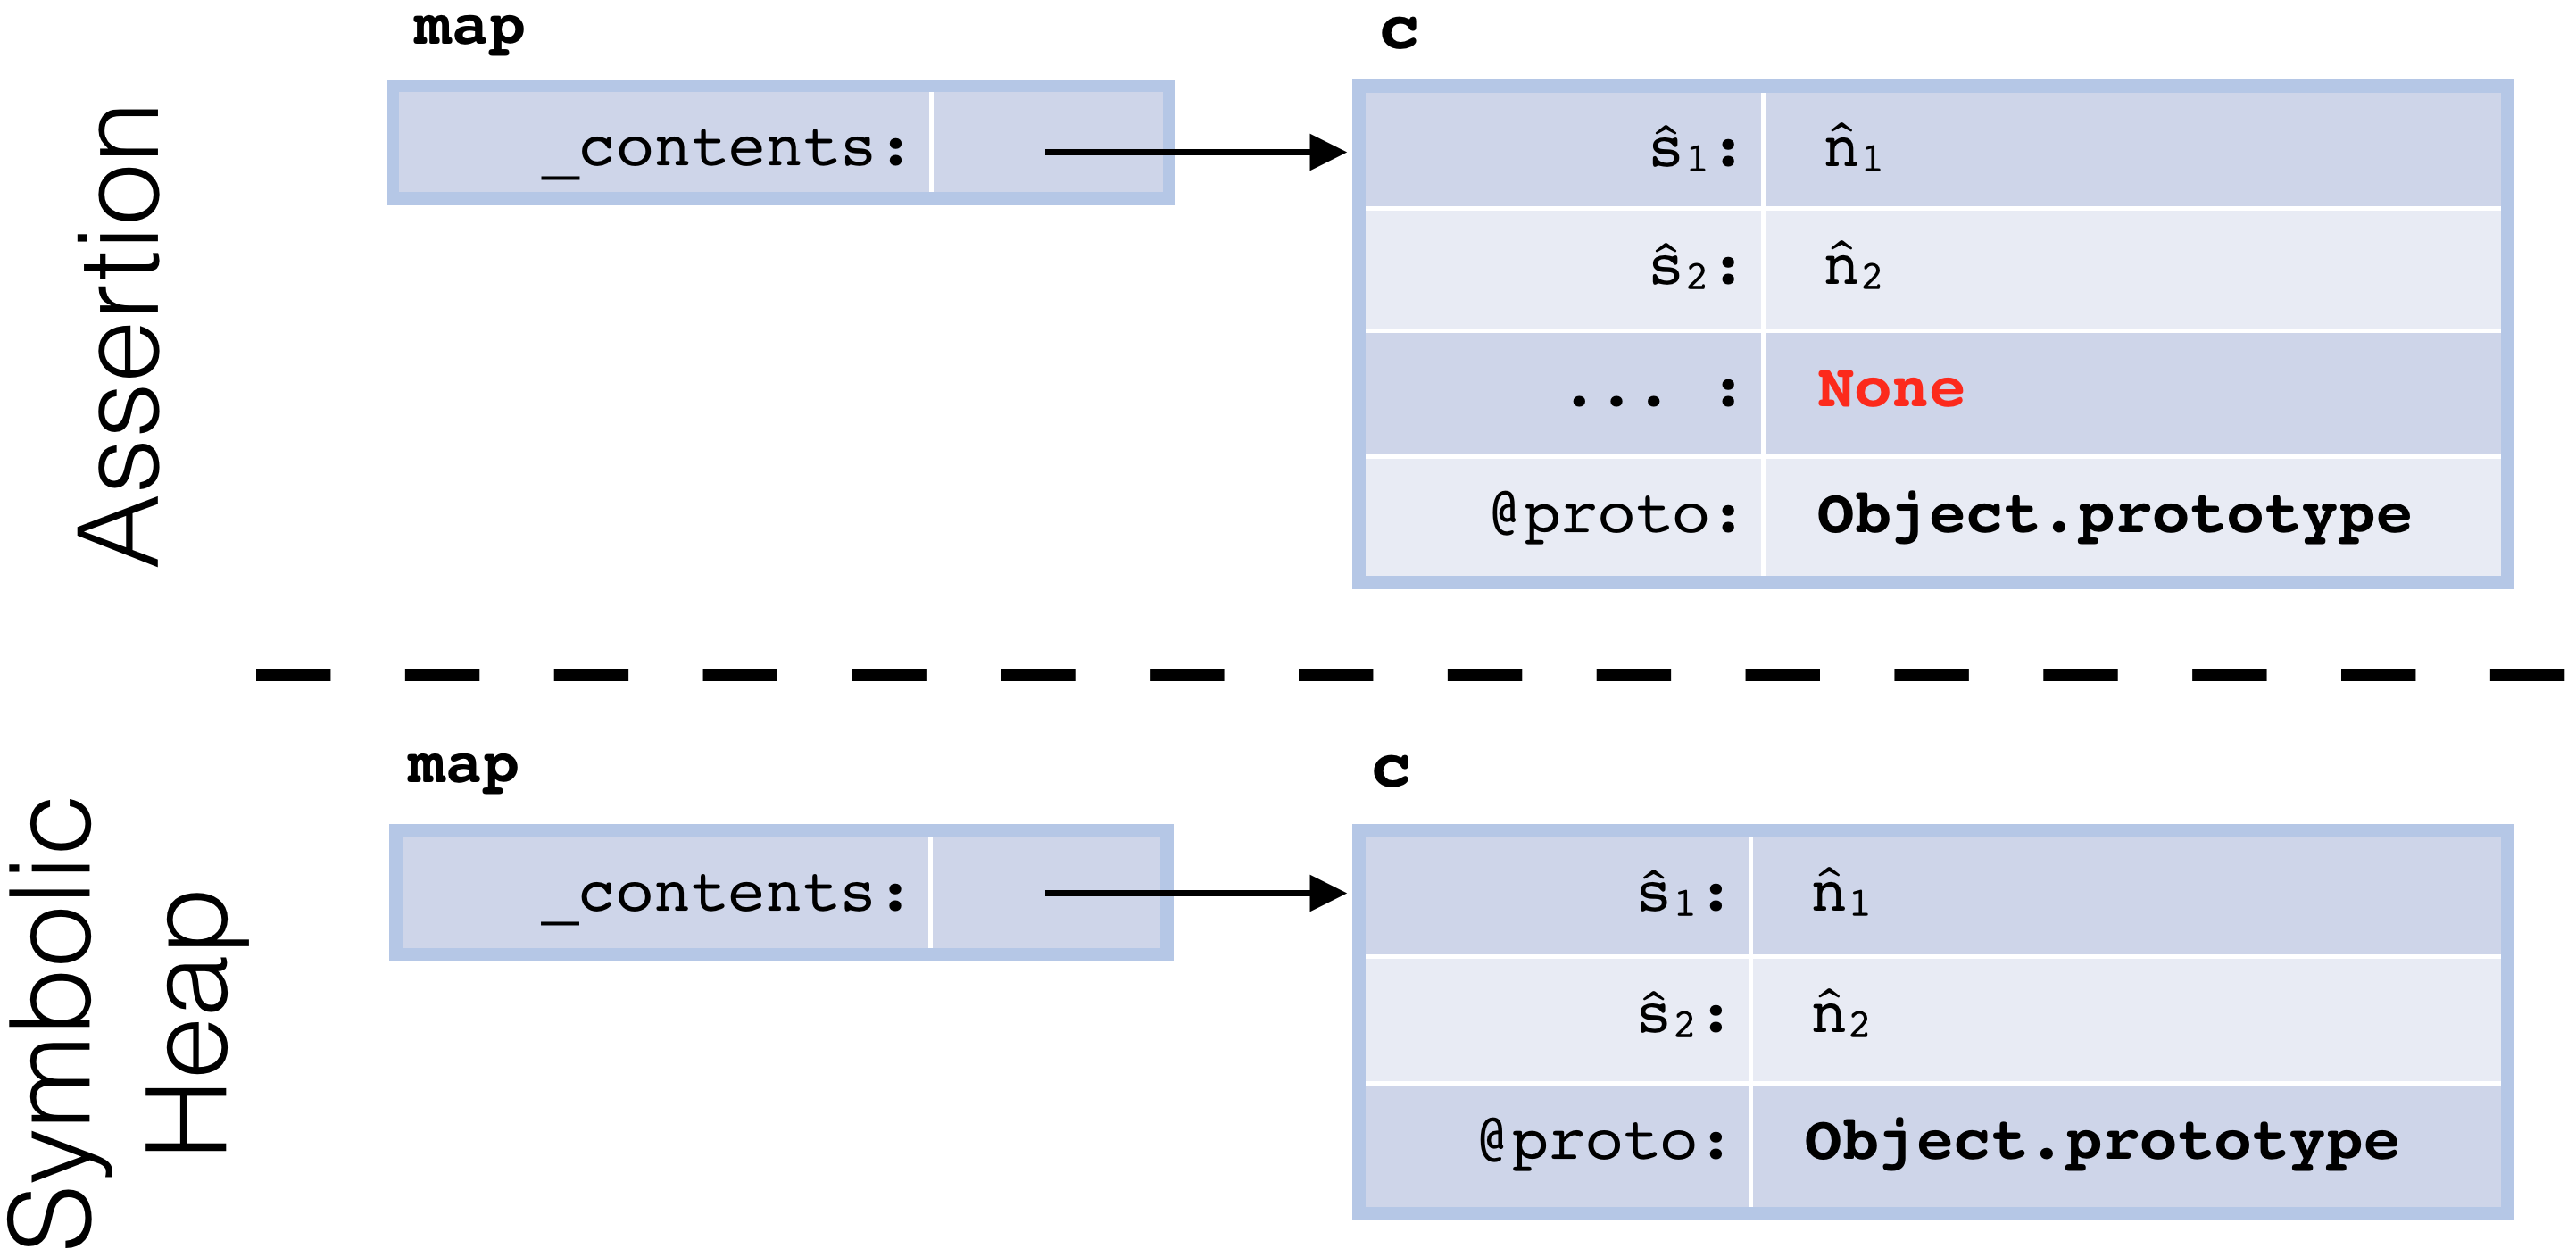
\includegraphics[width=\linewidth]{figures/symbvsass.png}

\vspace*{-0.7cm}
{\small $$
\text{\emph{Negative resource constraints: }} \{ \hat{s}_1, \hat{s}_2 \} \subseteq \{ \hat{s}_1, \hat{s}_2 \}
$$}
\vspace{-0.8cm}
\caption{Assertion vs. Symbolic Heap: {\small$\mathtt{Map(map, \{ (\hat{s}_1, \hat{n}_1), (\hat{s}_2, \hat{n}_2) \} )}$}}\label{fig:symb:state:versus:assertion}
\vspace{-0.5cm}
\end{figure}

\myparagraph{Example}
We illustrate the debugging of SL-specifications by appealing to the \jsinline|Map| example shown in Figure \ref{map:example}. In order to reason about a key-value map,
we define several predicates, whose definitions we show below.

\begin{Verbatim}[fontsize=\footnotesize,commandchars=\\\{\}]
Map (m, kvs) := 
  DataProp(m, "_contents", c) * JSObject(c) * 
    KVPairs(c, kvs) * first(kvs, keys) * emptyFields(c, keys)
\end{Verbatim}
 \begin{Verbatim}[fontsize=\footnotesize,commandchars=\\\{\}]
KVPairs (o, kvs) := 
  (kvs = \{ \}),
  (kvs = (k, v) -u- kvs') * ValidKey(k) * DataProp(o, k, v) * KVPairs(o, kvs')
\end{Verbatim}
\begin{Verbatim}[fontsize=\footnotesize,commandchars=\\\{\}]
ValidKey (k) := types(k : Str) * \textcolor{red}{(k <> "hasOwnProperty")}
\end{Verbatim}

The \jsinline|Map| predicate captures the resource corresponding to a map object. 
Concretely, it first states that the map object has the property \jsinline|_contents|, which points to a default JavaScript object \jsinline|c|, using the predicates \jsinline|DataProp| and \jsinline|JSObject|. 
\jsinline|DataProp(o, p, v)| captures the property \jsinline|p| of object \jsinline|o| and states that it has value \jsinline|v|, while abstracting over other associated JavaScript internals, whereas \jsinline|JSObject(o)| states that the object \jsinline|o| is an extensible object of class \jsinline|"Object"|, whose prototype is \jsinline|Object.prototype| (for more details, see~\cite{javert}). 
Next, using the \jsinline|KVPairs| predicate (explained shortly), it states that \jsinline|c| holds the key-value pairs \jsinline|kvs|. Finally, it states that \jsinline|c| has no other properties except the keys present in \jsinline|kvs|. For this, it first obtains the set of keys from the set of key-value pairs \jsinline|kvs| using the predicate \jsinline|first(kvs, keys)|, which states that the first projection of \jsinline|kvs| equals \jsinline|keys| (its definition is standard), and then uses the \jsinline|emptyFields| assertion to state that all other properties are absent from the object.

The \jsinline|KVPairs(o, kvs)| predicate talks about key-value pairs of an object \jsinline|o|. 
It is defined recursively on the structure of \jsinline|kvs| and it has two definitions, separated by a comma. 
We have that \jsinline|kvs| is either empty or that it contains at least one key-value pair \jsinline|(k, v)|.\footnote{We write {\small\texttt{-u-}} for set union and omit the brackets around singleton sets.} 
In the latter case, we state that the key \jsinline|k| must be valid, that the object \jsinline|o| has the property \jsinline|k| with value \jsinline|v|, and proceed recursively.
Note that the uniqueness of keys in \jsinline|kvs| is guaranteed by the \jsinline|DataProp| predicate of \jsinline|KVPairs| and the separating conjunction.

The \jsinline|ValidKey(k)| predicate captures the validity of a given key and holds \emph{iff} the corresponding JavaScript function \jsinline|validKey(k)| returns \jsinline|true|.
In the definition of \jsinline|ValidKey|, we highlight in red a potential source of errors on which we will focus shortly.

To give a better intuition of how the \jsinline|Map| predicate works, we show the full unfolding of {\small$\mathtt{Map(map, \{ (\hat{s}_1, \hat{n}_1), (\hat{s}_2, \hat{n}_2) \} )}$} in Figure \ref{fig:symb:state:versus:assertion}.
%a \emph{map object predicate}, \jsinline|Map|, 
%which uses the auxiliary predicate \jsinline|KVPairs|, capturing the resource of the key-value pairs in the map, 
%and the \jsinline|validKey(k)| predicate, which captures the validity of a key and holds if and only if the corresponding JavaScript function \jsinline|ValidKey(k)| returns \jsinline|true|\footnote{For the moment, we treat the $\mathtt{ValidKey}$ predicate as a black box.}.
%
%Intuitively, the \jsinline|Map(m, kvs)| predicate captures the resource 
%of a map object \jsinline|m| with key-value pairs \jsinline|kvs| (a set of string-number pairs, modelled as two-element lists).
%%\footnote{We model pairs as lists with two elements and, for clarity, use the pair notation.}). 
%For instance, the assertion $\mathtt{Map(map, \{ (\hat{s}_1, \hat{n}_1), (\hat{s}_2, \hat{n}_2) \} )}$ can be unfolded as illustrated in Figure~\ref{fig:symb:state:versus:assertion}. 
%Observe that the definition of \jsinline|Map| does not include the resource of a map prototype, as it is shared between all map objects, and therefore needs to be factored out.  
%
There, we can also see how the negative resource captured by the SL-assertion {\small$\mathtt{Map(map, \{ (\hat{s}_1, \hat{n}_1), (\hat{s}_2, \hat{n}_2) \} )}$}, namely the resource captured by {\small$\mathtt{emptyFields(c, first(kvs))}$}, disappears from the symbolic heap and is transformed into the negative resource constraint $\{ \hat{s}_1, \hat{s}_2 \} \subseteq \{ \hat{s}_1, \hat{s}_2 \}$, which states that all properties of the object \jsinline|c| in the symbolic heap (in our case, $\hat{s}_1$ and $\hat{s}_2$) must be in the set of properties of the corresponding \jsinline|emptyFields| assertion (in our case, {\small$\mathtt{first(\{ (\hat{s}_1, \hat{n}_1), (\hat{s}_2, \hat{n}_2) \}) = \{ \hat{s}_1, \hat{s}_2 \}}$}).
Such constraints are generated in item ${\bf e.}$ of the test generation algorithm presented in Figure \ref{fig:test:generation}. 

Below, we show the relevant parts of the specifications of \jsinline|get(k)| and \jsinline|put(k, v)|, for the case in which
 \jsinline|k| already exists in the map:

\noindent
\begin{minipage}{\linewidth}
\begin{displaymath} 
{\scriptsize
\hspace*{-0.2cm}
\begin{array}{c}
\left\{ {\begin{array}{c}
 \text{\texttt{Map(this, kvs -u- (k, v)) * ObjProtoF() *}} \\
 \text{\texttt{(this, "@proto") -> mp * MapProto(mp) * ...}}
\end{array}} \right\} \\
%
\text{\bfseries \texttt{get(k)}} \\[0.2mm]
%
\left\{ {\begin{array}{c}
 \text{\texttt{Precondition * (ret = v)}} 
\end{array}} \right\}
\end{array}
} 
\end{displaymath}
\end{minipage}
\quad
\begin{minipage}{\linewidth}
%
\begin{displaymath} 
{\scriptsize
\begin{array}{c}
\left\{ {\begin{array}{c}
 \text{\texttt{Map(this, kvs -u- (k, v')) * ObjProtoF() *}} \\
 \text{\texttt{(this, "@proto") -> mp * MapProto(mp) * ...}}
\end{array}} \right\} \\
%
\text{\bfseries \texttt{put(k, v)}} \\[0.2mm]
%
\left\{ {\begin{array}{c}
 \text{\texttt{Map(this, kvs -u- (k, v)) * ObjProtoF() *}} \\
 \text{\texttt{(this, "@proto") -> mp * MapProto(mp) * ...}}
\end{array}} \right\}
\end{array}
} 
\end{displaymath}
\end{minipage}

\vspace{10pt}
The predicate \jsinline|ObjProtoF()| describes the resource captured by the \jsinline|Object.prototype| object. 
In particular, it is needed because \texttt{get} uses the \texttt{hasOwnProperty} function, which is defined as a property of \jsinline|Object.prototype|. 
The predicate \jsinline|MapProto| specifies the resource of a valid map prototype: in particular, the map prototype needs to define the methods \jsinline|put|, \jsinline|get|, and \jsinline|validKey|. Finally, note that, given the definition of the \jsinline|Map| and \jsinline|KVPairs| predicates, both preconditions shown entail that \jsinline|k| is a valid key.

\begin{figure}[t!]
\centering
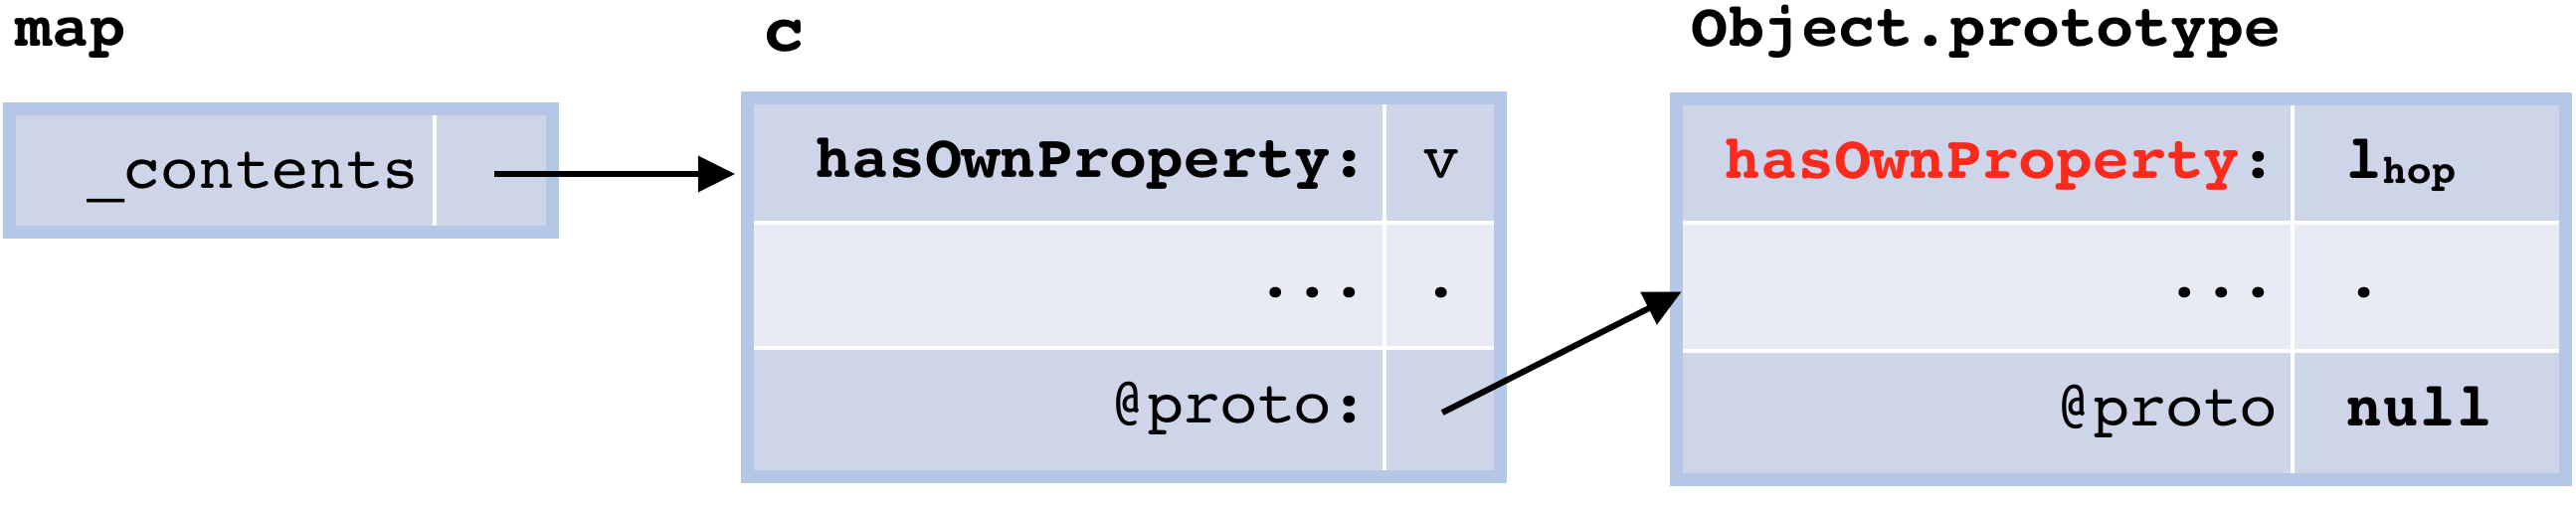
\includegraphics[width=\linewidth]{figures/heapfail.png}
\caption{Property shadowing: \jsinline|c.hasOwnProperty(...)| cannot reach \jsinline|Object.prototype|.} 
\label{fig:cexget}
\vspace{-0.5cm}
\end{figure}

Now, if we forgot to state the part of the $\mathtt{ValidKey(k)}$ predicate highlighted in red, that is, if we did not state that $\mathtt{k}$ needed to be different from \jsinline|"hasOwnProperty"|, the symbolic test generated for the specification of \jsinline|get| would fail for unfoldings of $\mathtt{KVPairs}$ of depth $\geq 1$, with the counter-model \jsinline|k = "hasOwnProperty"|. 
In that case, as illustrated in Figure~\ref{fig:cexget}, the \jsinline|"hasOwnProperty"| property of \jsinline|Object.prototype| would no longer be reachable by property lookup from \jsinline|c|, and
the execution of line~5 (\jsinline|if (c.hasOwnProperty(k))|) would raise an error, as it would attempt to call the \jsinline|"hasOwnProperty"| property of object \jsinline|c| as a function instead. 
Since this specification of $\mathtt{get(k)}$ requires normal termination, the jump to the error label in the compiled \jsil code will trigger the $\assert(\jfalse)$ of the generated symbolic test and the developer will be presented with the counter-model \jsinline|k = "hasOwnProperty"|.

\begin{center}
\polish{What else would we like to say here?}
\end{center}


\clearpage
\newpage

\section{OLD -- Symbolic Execution for \jsil}\label{sec:jsil:symb:exec}
%!TEX root = ../main.tex

We introduce our symbolic execution engine for \jsil~\cite{javert}. In~\S\ref{subsec:jsil:analysis:formalism}, we present 
the theoretical underpinnings of the symbolic analysis, including
a soundness result and a guarantee of absence of false 
positives for bug-finding.
In \S\ref{subsec:jsil:analysis:implementation}, 
we describe the implementation of the \jsil symbolic analysis 
in \rosette~\cite{Rosette1,Rosette2}.

\vspace*{-0.2cm}
\subsection{Formalisation}\label{subsec:jsil:analysis:formalism}

\vspace*{-0.2cm}
\myparagraph{\jsil: Syntax} \jsil is a simple goto language featuring top-level procedures and commands operating on object heaps. It was purposefully designed to natively support the main dynamic features of JavaScript: extensible objects; dynamic property access; and dynamic procedure calls. The syntax of \jsil is shown in Figure \ref{def:jsil-types}.

\jsil \emph{values}, $\val \in \vals$, include numbers, booleans, strings, the special values $\jsundefined$ and $\jsnull$, as well as types~$\ivltype$, procedure identifiers $\fid$, and the special value $\jsilempty$. 
\jsil~\emph{expressions}, $\jsilexpr \in \exprs$, include \jsil values, \jsil program variables $\jvar$, and various unary and binary operators, which, for instance, provide support for sets and lists. 


%\pg{When talking about JSIL Logic, how are you going to explain the difficulty associated with a dynamci goto language v a static one, I don't think your work is a boring adaptation of reasoning about a staitc goto language. You need to grab at some of this is you can. We've have not paid ebough attention on this, so people jsut think this is a variant of previous work..} 

\begin{figure*}[!t]
\begin{minipage}{\textwidth}
\centering
\begin{tabular}{lllll}
	 Numbers: $\jnumber \in \numbers$ &  Booleans: $\jbool \in \bools$ & \  \ Strings: $\jstring \in \strings$ & \  \ Locs: $\loc \in \locs$ & \  Vars: $\jvar \in \jvars$ \\[0.1cm]
	Types: $\ivltype \in \ivltypes$ & \multicolumn{4}{l}{Values: $\val \in \vals$ \defeq \ $\jnumber \mid \jbool \mid \jstring \mid  \jsundefined \mid \jsnull \mid \loc \mid \ivltype \mid \fid \mid \jsilempty$} \\[0.1cm]
\multicolumn{5}{l}{Expressions: $\jsilexpr \in \exprs$ \defeq \ $\val \mid \jvar \mid \ominus\ \jsilexpr \mid \jsilexpr \binop{} \jsilexpr $} \\[0.1cm]
	\multicolumn{5}{l}{Basic Commands: $\bcmd \in \bcmds$ \defeq\ $\jsilskip \mid \jvar := \jsilexpr  \mid \jvar := \jsilnew() \mid \jvar := [\jsilexpr, \jsilexpr] \mid [\jsilexpr, \jsilexpr] := \jsilexpr \mid$} \\[0.1cm]
	\multicolumn{5}{l}{\hspace{2.8cm} $\jsildelete(\jsilexpr, \jsilexpr) \mid \jvar := \hasfield(\jsilexpr, \jsilexpr) \mid \jvar := \getfields(\jsilexpr) \mid \assume(\jsilexpr) \mid \assert(\jsilexpr)$} \\[0.1cm]
	% Commands
	\multicolumn{5}{l}{Commands: $\ivlcmd \in \cmds$ \defeq \ $ \bcmd \mid \goto \ i \mid  \ifgoto{\jsilexpr}{i}{j} \mid \jsilcall{\jvar}{\jsilexpr}{\jvec{\jsilexpr}}{j}$} \\[0.1cm]
	\multicolumn{5}{l}{Procedures : $\proc \in \procset$ \defeq \ $\procedure{\fid}{\jvec{\jvar}}{\jvec{\ivlcmd}}$}
 \end{tabular}
 \vspace*{-0.1cm}
 \caption{Syntax of the \jsil Language}
 \label{def:jsil-types}
 \vspace*{-0.5cm}
 \end{minipage}
 \end{figure*}
 
%Most syntactic constructs of JSIL either come directly from JavaScript or are useful for JavaScript analysis. 


\jsil \emph{basic commands} enable the manipulation of extensible objects and do not affect control flow. 
They include $\jsilskip$, variable assignment, object creation, property access, property assignment, property deletion, membership check, property collection, and two special commands, $\assume$ and $\assert$, essential for symbolic execution, but with trivial concrete semantics.
%
\jsil \emph{commands} include \jsil basic commands and several commands related to control flow: conditional gotos, unconditional gotos and dynamic procedure calls.\footnote{\jsil also has a $\phi$-node assignment, which allows \JSComp to produce code directly in Static-Single-Assignment (SSA) \cite{SSA}. To avoid clutter, we omit the $\phi$-node assignment from this formalisation as it does not impact the reasoning in any way. Details can be found in \cite{javert}.} 
The two goto commands are straightforward: $\goto \ i$ jumps to the $i$-th command of the active procedure, and $\ifgoto{\jsilexpr}{i}{j}$ jumps to the $i$-th command if $\jsilexpr$ evaluates to $\jtrue$, and to the $j$-th if it evaluates to $\jfalse$. 
The dynamic procedure call $\jsilcall{\jvar}{\jsilexpr}{\jvec{\jsilexpr}}{j}$ first evaluates  $\jsilexpr$ and $\jvec{\jsilexpr}$ to obtain the procedure name and arguments, respectively, executes the appropriate procedure with these arguments, and, in the end, assigns its return value to $\jvar$.
If the procedure raises an error, control is transferred to the $j$-th command, and to the next otherwise. 

A \jsil program $\prog \in \ivlprogs$ can be seen as a set of top-level procedures of the form $\procedure{\fid}{\jvec{\jvar}}{\jvec{\jcmd}}$, where $\fid$ is the procedure name, $\jvec{\jvar}$ are its formal parameters, and its body ${\jvec{\jcmd}}$  is a \emph{command list} consisting of a sequence of \jsil commands.
Every \jsil program contains a special procedure $\jsilmain$\hspace{-2pt}, denoting the entry point of the program. 
\jsil procedures return via two dedicated indexes, $\procretlab$ and $\procerrlab$, using two dedicated variables, $\procretvar$ and $\procerrvar$. If a procedure reaches the $\procretlab$ index, it returns normally with the return value denoted by $\procretvar$; when it reaches $\procerrlab$, it returns an error, with the error value denoted by $\procerrvar$.

\myparagraph{\jsil: Semantics}
The basic memory model of \jsil is as follows. 
%\jsil values contain: numbers, $\jnumber$; booleans, $\jbool$; strings, $\jstring$;  the special values \jsinline|undefined| and \jsinline|null|; and object locations,  $\loc \in \locs$.
A \jsil heap, $\heap \in \heaps$, is a partial function mapping pairs of  object locations, and strings to heap values. 
 Given a heap~$\heap$, we denote: a heap cell by $\hcell{\loc}{\jstring}{\val}$, meaning that  $h(\loc,\jstring) = \val$; the union of two disjoint heaps by $\oheap_1 \dunion \oheap_2$; heap lookup by $\hread{\oheap}{\loc}{\jstring}$; and the empty heap by $\hemp$.
A \jsil variable store, $\store \in \stores$, is a mapping from JSIL program variables $\jvar \in \jvars$ to JSIL values. Finally, \jsil has two execution modes, ranged over by $\mode$: $\top$, which indicates that the execution can proceed; and~$\bot$, which indicates that a failure has occurred and the execution must stop. 

\jsil semantics is defined in small-step style. Transitions for basic commands, given in Figure \ref{fig:sem:basic:commands}, are of the form $\semtrans[\mode][\mode']{\heap, \store, \bcmd}{\heap', \store'}$, meaning that the execution of the basic command $\bcmd$ in the heap $\heap$, store $\store$, and execution mode $\mode$ results in the heap $\heap'$, $\store'$, and execution mode $\mode'$. 
We denote the semantic interpretation of unary operators $\unoper$ by $\semop{\unoper}$, the semantic interpretation of binary operators $\binoper$ by $\semop{\binoper}$.

\begin{figure}[t!]
{\scriptsize
\begin{mathpar} 
%
\inferrule[Evaluation of expressions]{}{
\semexpr{\val}{\store} \semeq \val
\quad 
\semexpr{\jvar}{\store} \semeq \store(\jvar)
\quad 
\semexpr{\unoper\ \jexpr}{\store} \semeq \semop{\unoper} (\semexpr{\jexpr}{\store})
\quad 
\semexpr{\jexpr_1 \binoper \jexpr_2}{\store} \semeq \semop{\binoper}(\semexpr{\jexpr_1}{\store}, \semexpr{\jexpr_2}{\store})}
\\

\inferrule[\textsc{Skip}]{}
	{ \semtrans[][\top]{\heap, \store, \jsilskip}{\heap, \store}} 
 \qquad
%
\inferrule[\textsc{Object Creation}]
  { 
    \heap = \heap \dunion \hcell{\loc}{\protop}{\jsnull}
    \quad (\loc,-) \notin \domain (\heap)
  }{\semtrans[][\top]{\heap, \store, \jvar := \jsilnew()}{\heap, \store[\jvar \mapsto \loc]}}
\\
\vspace*{-0.1cm}
\inferrule[\textsc{Property Collection}]
  {
      \symbeval{\jsilexpr}{\store} =  \loc
      \quad
        \heap = \heap' \, \uplus \, \big((l, \jstring_i) \mapsto \val_i\big)\mid_{i = 0}^n   
        \quad
        (l, -) \not\in \domain(\heap')
  }{\semtrans[][\top]{\heap, \store, \jvar := \getfields(\jsilexpr)}{\heap, \store[\jvar \mapsto \jsilset{\jstring_0, ..., \jstring_n}]}} 
%
\qquad
 %
\inferrule[\textsc{Assignment}]
  {
      \symbeval{\jsilexpr}{\store} =  \val
      \quad
      \store' = \store[\jvar \mapsto \val]
  }{\semtrans[][\top]{\heap, \store, \jvar := \jsilexpr}{\heap, \store'}} 
\\
%
\inferrule[\textsc{Property Access}]
  { 
 	\symbeval{\jsilexpr_1}{\store} =  \loc
  	\quad 
        \symbeval{\jsilexpr_2}{\store} =  \jstring
        \quad
        \heap = - \dunion \hcell{\loc}{\jstring}{\val}
  }{ \semtrans[][\top]{\heap, \store, \jvar := [\jsilexpr_1, \jsilexpr_2]}{\heap,  \store[\jvar \mapsto \val]}}
 \and 
 \inferrule[\textsc{Property Deletion}]
  { 
        \symbeval{\jsilexpr_1}{\store} =  \loc
  	\quad 
        \symbeval{\jsilexpr_2}{\store} =  \jstring
        \quad
        \heap = \heap' \dunion \hcell{\loc}{\jstring}{-}
  }{\semtrans[][\top]{\heap, \store, \jsildelete(\jsilexpr_1, \jsilexpr_2)}{\heap', \store}}
 %
\\
%
\inferrule[\textsc{Property Assignment - Found}]
  {     \symbeval{\jsilexpr_1}{\store} =  \loc
  	\quad 
        \symbeval{\jsilexpr_2}{\store} =  \jstring
        \quad
        \symbeval{\jsilexpr_3}{\store} =  \val
       \\\\
        \heap = \heap' \dunion  \hcell{\loc}{\jstring}{-}
  }{\semtrans[][\top]{\heap, \store, [\jsilexpr_1, \jsilexpr_2] := \jsilexpr_3}{\heap' \dunion  \hcell{\loc}{\jstring}{\val}, \store}} 
 \and 
 \inferrule[\textsc{Property Assignment - Not Found}]
  {     \symbeval{\jsilexpr_1}{\store} =  \loc
  	\quad 
        \symbeval{\jsilexpr_2}{\store} =  \jstring
        \quad
        \symbeval{\jsilexpr_3}{\store} =  \val
       \\\\
        \heap = \heap' 
        \quad 
        (\loc, \jstring) \not\in \domain(\heap)
  }{\semtrans[][\top]{\heap, \store, [\jsilexpr_1, \jsilexpr_2] := \jsilexpr_3}{\heap \dunion  \hcell{\loc}{\jstring}{\val}, \store}} 
\\
%
\inferrule[\textsc{Member Check - True}]
  { 
      \symbeval{\jsilexpr_1}{\store} =  \loc
  	\quad 
        \symbeval{\jsilexpr_2}{\store} =  \jstring
       \quad 
   	(\loc, \jstring) \in \domain(\heap) 
  }{\semtrans[][\top]{\heap, \store,\jvar := \hasfield(\jsilexpr_1, \jsilexpr_2)}{\heap, \store[\jvar \mapsto \jtrue]}}
  \and 
 \inferrule[\textsc{Member Check - False}]
  { 
      \symbeval{\jsilexpr_1}{\store} =  \loc
  	\quad 
        \symbeval{\jsilexpr_2}{\store} =  \jstring
       \quad 
   	(\loc, \jstring) \not\in \domain(\heap) 
  }{\semtrans[][\top]{\heap, \store,\jvar := \hasfield(\jsilexpr_1, \jsilexpr_2)}{\heap, \store[\jvar \mapsto \jfalse]}}
%
\\
%
\inferrule[\textsc{Assert - True}]
  { 
      \symbeval{\jsilexpr}{\store} =  \jtrue
  }{\semtrans[][\top]{\heap, \store, \assert(\jsilexpr)}{\heap, \store}} 
\and
\inferrule[\textsc{Assert - False}]
  { 
      \symbeval{\jsilexpr}{\store} = \jfalse
  }{\semtrans[][\top][\bot]{\heap, \store, \assert(\jsilexpr)}{\heap, \store}}
\and
 \inferrule[\textsc{Assume}]
  { 
      \symbeval{\jsilexpr}{\store} =  \jtrue
  }{\semtrans[][\top]{\heap, \store, \assume(\jsilexpr)}{\heap, \store}} 

\end{mathpar}}
\vspace*{-0.5cm}
\caption{Execution for Basic Commands: {\scriptsize$\semtrans[][\mode][\mode']{\heap, \store, \bcmd}{\heap', \store'}$}\label{fig:sem:basic:commands}}
\vspace*{-0.5cm}
\end{figure}

To describe transitions for \jsil commands, we introduce call stacks, denoted~$\ctx$.
Call stacks are lists of tuples of the form $(\pid, \store, \jvar, i, j)$, where: 
\dtag{1}~$\pid$~is a procedure identifier;
\dtag{2}~$\store$~is the store of the procedure that called $\pid$; 
\dtag{3}~$\jvar$~is the variable to which the return of $\pid$ must be assigned in $\store$; 
\dtag{4} $i$ is the index 
of the command to which the control must jump after the execution of $\pid$ in 
case of normal return; 
and \dtag{5} $j$ the index to which it must jump in case of 
error return. Transitions for control flow commands have the form:  $\semtrans[\prog][\mode][\mode']{\heap, \store, i}{\heap', \store', i'}[\ctx][\ctx']$, meaning that, in the context of the entire program $\prog$, the evaluation of the $i$-th command of the first procedure in the call stack $\ctx$, in
the heap $\heap$, store $\store$, and execution mode $\mode$, generates the heap $\heap'$, store $\store'$, call stack $\ctx'$,   
and the next command to be evaluated is the $i'$-th command of the first procedure of the call stack~$\ctx'$, in execution mode $\mode'$. Due to space constraints and as the transitions for JSIL symbolic execution are  similar, we give the full semantics for JSIL control flow commands in the~Appendix. % So far, so boring.

\myparagraph{\jsil: Symbolic Semantics}
In order to symbolically execute \jsil programs, we extend the syntax of \jsil expressions with 
symbolic strings $\sstring \in \sstrings$ and symbolic numbers $\snumber \in \snumbers$. 
For convenience, we use $\svars$ to denote the union of $\sstrings$ and $\snumbers$ 
and $\svar$ to range over $\svars$. We introduce: \jsil symbolic expressions, $\sexpr \in \sexprs$, defined as follows: $\sexpr \triangleq \val \mid \svar \mid \unoper\ \sexpr \mid \sexpr \binoper \sexpr$; as well as \jsil extended symbolic expressions, $\pvsexpr \in \pvsexprs$, defined as follows: $\pvsexpr \triangleq \val \mid \jvar \mid \svar \mid \unoper\ \pvsexpr \mid \pvsexpr \binoper \pvsexpr$. Extended expressions differ from symbolic ones in that they can contain program variables.

We extend heaps, stores, and call stacks with symbolic values, obtaining symbolic 
heaps, stores, and call stacks, respectively ranged over by $\sheap$, $\sstore$, and $\sctx$. 
A symbolic heap, $\sheap \in \sheaps$, is a partial function mapping pairs of  
object locations and symbolic expressions to symbolic expressions. 
A symbolic store, $\sstore \in \sstores$, is a mapping from program variables 
$\jvar \in \jvars$ to symbolic expressions. Therefore, an evaluation of a \jsil extended expression $\pvsexpr$ in a symbolic store $\sstore$ always yields a 
symbolic expression $\sexpr$.
A symbolic call stack $\sctx$ only differs from a concrete call stack in that it contains 
symbolic stores instead of concrete stores.
%

%Figure~\ref{fig:symb:sem:exprs} shows the rules for symbolically evaluating \jsil expressions. 

%
A \emph{symbolic state} $\sstate = (\sheap, \sstore, \sctx, \pc)$ is a 4-tuple consisting of a 
symbolic heap $\sheap$, a symbolic store $\sstore$, a symbolic call stack $\sctx$, and a path condition $\pc$. 
The \emph{path condition}~\cite{symb:exec:survey} is a first-order quantifier-free formula over symbolic strings and 
numbers, which accumulates constraints on the given symbolic inputs that trigger 
the execution to follow the path that led to the current symbolic state. 
Path conditions are given by the following grammar: 
\begin{equation*}
\pc \triangleq \sexpr_1 = \sexpr_2 \mid \sexpr_1 \leq \sexpr_2 \mid \pc_1 \, \wedge \, \pc_2 \mid \pc_1 \vee \pc_2 \mid \neg \pc \mid \jtrue \mid \jfalse
\end{equation*}

\begin{figure*}[!t]
{\scriptsize
\begin{mathpar} 
%
\inferrule[\textsc{Evaluation of extended \jsil expressions}]{}{
%
{\begin{array}{c}
\semexpr{\val}{\sstore} \semeq \val \\[2pt]
%
\semexpr{\xvar}{\sstore} \semeq \sstore(\xvar) \\[2pt]
%
\semexpr{\svar}{\sstore} \semeq \svar
\end{array}}
%
\qquad
%
\frac{\semexpr{\pvsexpr}{\sstore} = \val}
      {\semexpr{\unoper\ \pvsexpr}{\sstore} \semeq \semop{\unoper} \val}
%
\qquad
%
\frac{\semexpr{\pvsexpr}{\sstore} = \sexpr \not\in \vals}
       {\semexpr{\unoper\ \pvsexpr}{\sstore} \semeq \unoper \ \sexpr}
%
\qquad
\frac{ \val = \semop{\binoper}(\semexpr{\pvsexpr_1}{\sstore}, \semexpr{\pvsexpr_2}{\sstore})} 
       {\semexpr{\pvsexpr_1 \binoper \pvsexpr_2}{\sstore} \semeq \val}
 %
 \qquad
\frac{{\begin{array}{c}
	\semexpr{\pvsexpr_1}{\sstore} = \sexpr_1 
	  \quad 
	  \semexpr{\pvsexpr_2}{\sstore} = \sexpr_2
	  \\
	  \sexpr_1 \not\in \vals \ \vee \ \sexpr_2 \not\in \vals 
	  \end{array}}
	}
	{\semexpr{\pvsexpr_1 \binoper \pvsexpr_2}{\sstore} \semeq \sexpr_1 \, {\binoper} \, \sexpr_2}
}
%
\\
%
\inferrule[\textsc{Skip}]{}
	{ \symbtrans[][\top]{\sheap, \sstore, \jsilskip, \pc}{\sheap, \sstore, \pc}} 
 \and
%
\inferrule[\textsc{Object Creation}]
  { 
    (\loc,-) \notin \domain (\sheap) 
    \and
    \sheap' = \sheap \dunion \hcell{\loc}{\protop}{\jsnull}
    \and 
  }{\symbtrans[][\top]{\sheap, \sstore, \jvar := \jsilnew(), \pc}{\sheap', \sstore[\jvar \mapsto \loc], \pc}}
\\
\inferrule[\textsc{Assignment}]
  {
      \symbeval{\pvsexpr}{\sstore} =  \sexpr
      \quad
      \sstore' = \sstore[\jvar \mapsto \sexpr]
  }{\symbtrans[][\top]{\sheap, \sstore, \jvar := \pvsexpr, \pc}{\sheap, \sstore', \pc}} 
  %
  \and
  %
  \inferrule[\textsc{Property Collection}]
  {
      \symbeval{\pvsexpr}{\sstore} =  \loc
      \quad
        \sheap = \sheap' \, \uplus \, \big((l, \sexprp_i) \mapsto - \big)\mid_{i = 0}^n   
        \quad
        (l, -) \not\in \domain(\sheap')
  }{\semtrans[][\top]{\heap, \store, \jvar := \getfields(\pvsexpr), \pc}{\heap, \store[\jvar \mapsto \jsilset{\sexprp_0, ..., \sexprp_n}],\pc}} 
%
\\
\inferrule[\textsc{Property Access}]
  { 
 	\symbeval{\pvsexpr_1}{\sstore} =  \loc
  	\quad 
        \symbeval{\pvsexpr_2}{\sstore} =  \sexpr_p
        \quad
        \sheap = \sheap' \, \uplus \, \big((l, \sexprp_i) \mapsto \sexprv_i\big)\mid_{i = 0}^n   
        \quad
        (l, -) \not\in \domain(\sheap')
        \quad 
        0 \leq k \leq n
        \\\\
        \pc' = \pc \ \wedge \, \big( (\sexprp_k = \sexpr_p) \ \wedge \left(\wedge_{i = 0, i \neq k}^n (\sexprp_i \neq \sexpr_p) \right)\big)
  }{ \symbtrans[][\top]{\sheap, \sstore, \jvar := [\pvsexpr_1, \pvsexpr_2], \pc}{\sheap,  \sstore[\jvar \mapsto \sexprv_k], \pc'}}
 %
\\
%
\inferrule[\textsc{Property Assignment - Found}]
  {     \symbeval{\pvsexpr_1}{\sstore} =  \loc
  	\quad 
        \symbeval{\pvsexpr_2}{\sstore} =  \sexpr_p
        \quad
        \symbeval{\pvsexpr_3}{\sstore} =  \sexpr_v
       \quad 
        \sheap = \sheap' \, \uplus \, \big((l, \sexprp_i) \mapsto \sexprv_i\big)\mid_{i = 0}^n   
        \quad
        (l, -) \not\in \domain(\sheap')
        \quad 
        0 \leq k \leq n
        \\
          \pc' = \pc \ \wedge \, \big( (\sexprp_k = \sexpr_p) \ \wedge \left( \wedge_{i = 0, i \neq k}^n (\sexprp_i \neq \sexpr_p) \right)\big)
         \quad
         \sheap'' = \sheap' \, \uplus \,  \big((l, \sexprp_i) \mapsto \sexprv_i\big)\mid_{i = 0, i \neq k}^n \, \uplus \,  (l, \sexpr_p) \mapsto \sexpr_v
  }{\symbtrans[][\top]{\sheap, \sstore,  [\pvsexpr_1, \pvsexpr_2] := \pvsexpr_3, \pc}{\sheap'', \sstore, \pc'}} 
\\
%
\inferrule[\textsc{Property Assignment - Not Found}]
  {     \symbeval{\pvsexpr_1}{\sstore} =  \loc
  	\quad 
        \symbeval{\pvsexpr_2}{\sstore} =  \sexpr_p
        \quad
        \symbeval{\pvsexpr_3}{\sstore} =  \sexpr_v
       \quad 
        \sheap = \sheap' \, \uplus \, \big((l, \sexprp_i) \mapsto \sexprv_i\big)\mid_{i = 0}^n   
        \quad
        (l, -) \not\in \domain(\sheap')
        \quad 
        0 \leq k \leq n
        \\
          \pc' = \pc \ \wedge \, \left(\wedge_{i = 0}^n (\sexprp_i \neq \sexpr_p)\right)
         \quad
         \sheap'' = \sheap \, \uplus \,  (l, \sexpr_p) \mapsto \sexpr_v
  }{\symbtrans[][\top]{\sheap, \sstore, [\pvsexpr_1, \pvsexpr_2] := \pvsexpr_3, \pc}{\sheap'', \sstore, \pc'}}   
%
\\
%
\inferrule[\textsc{Property Deletion}]
  { 
        \symbeval{\pvsexpr_1}{\sstore} =  \loc
  	\quad 
        \symbeval{\pvsexpr_2}{\sstore} =  \sexpr_p
       \quad 
        \sheap = \sheap' \, \uplus \, \big((l, \sexprp_i) \mapsto -\big)\mid_{i = 0}^n   
        \quad
        (l, -) \not\in \domain(\sheap')
        \quad 
        0 \leq k \leq n
     \\ 
      \pc' = \pc \ \wedge \, \big( (\sexprp_k = \sexpr_p) \ \wedge \left(\wedge_{i = 0, i \neq k}^n (\sexprp_i \neq \sexpr_p) \right)\big)
     \quad 
      \sheap'' = \sheap' \, \uplus \,  \big((l, \sexprp_i) \mapsto \sexprv_i\big)\mid_{i = 0, i \neq k}^n
   }{\symbtrans[][\top]{\sheap, \sstore, \jsildelete(\pvsexpr_1, \pvsexpr_2), \pc}{\sheap'', \sstore, \pc'}}
 \\
 %
\inferrule[\textsc{Member Check - True}]
  { 
      \symbeval{\pvsexpr_1}{\sstore} =  \loc
  	\quad 
        \symbeval{\pvsexpr_2}{\sstore} =  \sexpr_p
       \quad 
        \sheap = \sheap' \, \uplus \, \big((l, \sexprp_i) \mapsto -\big)\mid_{i = 0}^n   
        \quad
        (l, -) \not\in \domain(\sheap')
        \quad 
        0 \leq k \leq n
     \\ 
     \pc' = \pc \ \wedge \, \big( (\sexprp_k = \sexpr_p) \ \wedge \left(\wedge_{i = 0, i \neq k}^n (\sexprp_i \neq \sexpr_p) \right)\big)
  }{\symbtrans[][\top]{\sheap, \sstore, \jvar := \hasfield(\pvsexpr_1, \pvsexpr_2), \pc}{\sheap, \sstore[\jvar \mapsto \jtrue], \pc'}}
%
\\
%
\inferrule[\textsc{Member Check - False}]
  { 
      \symbeval{\pvsexpr_1}{\sstore} =  \loc
  	\quad 
        \symbeval{\pvsexpr_2}{\sstore} =  \sexpr_p
       \quad 
        \sheap = \sheap' \, \uplus \, \big((l, \sexprp_i) \mapsto -\big)\mid_{i = 0}^n   
        \quad
        (l, -) \not\in \domain(\sheap')
        \quad 
        0 \leq k \leq n
     \quad
     \pc' = \pc \ \wedge \,  \left(\wedge_{i = 0}^n (\sexprp_i \neq \sexpr_p)\right) 
  }{\symbtrans[][\top]{\sheap, \sstore, \jvar := \hasfield(\pvsexpr_1, \pvsexpr_2), \pc}{\sheap, \sstore[\jvar \mapsto \jfalse], \pc'}}
\\
%
\inferrule[\textsc{Assert - True}]
  { 
      \symbeval{\pvsexpr}{\sstore} =  \sexpr
     \quad 
     \pc \vdash \sexpr 
  }{\symbtrans[][\top]{\sheap, \sstore, \assert(\pvsexpr), \pc}{\sheap, \sstore, \pc}} 
\quad
\inferrule[\textsc{Assert - False}]
  { 
      \symbeval{\pvsexpr}{\sstore} =  \sexpr
     \quad 
     (\pc \, \wedge \,  \neg\sexpr) \text{ satisfiable}
  }{\symbtrans[][\top][\bot]{\sheap, \sstore, \assert(\pvsexpr), \pc}{\sheap, \sstore,  \pc \wedge \neg\sexpr}}
  \quad
%
\inferrule[\textsc{Assume}]
  { 
      \symbeval{\pvsexpr}{\sstore} =  \sexpr
     \quad 
     \pc \vdash \sexpr 
  }{\symbtrans[][\top]{\sheap, \sstore, \assume(\pvsexpr), \pc}{\sheap, \sstore, \pc \land \sexpr}} 
\end{mathpar}}
\vspace*{-0.4cm}
\caption{Symbolic Semantics for \jsil Basic Commands: {$\symbtrans[][\mode][\mode']{\sheap, \sstore, \bcmd, \pc}{\sheap', \sstore', \pc'}$}\label{fig:symbexe:bcmds}}
\vspace*{-0.4cm}
\end{figure*}
%\end{display}  



\begin{figure*}[ht]
{\scriptsize
\begin{mathpar} 
\inferrule[\textsc{Basic Command}]
   { 
     \ccmd{i} = \bcmd 
     \quad
     \symbtrans{\sheap, \sstore, \bcmd, \pc}{\sheap', \sstore', \pc'} 
   }{\symbtrans{\sheap, \sstore, i, \pc}{\sheap', \sstore', i+1, \pc'}}
%
   \qquad
  %
  \inferrule[\textsc{Basic Command - Fail}]
   { 
     \ccmd{i} = \bcmd 
     \quad
     \symbtranserr{\sheap, \sstore, \bcmd, \pc}{}{\pc}
   }{\symbtranserr{\sheap, \sstore, i, \pc}{}{\pc}}
 %
   \qquad
  %
  \inferrule[\textsc{Goto}]
   { \ccmd{i} = \goto \, j \quad}
   {\symbtrans{\sheap, \sstore, i, \pc}{\sheap, \sstore, j, \pc}}
  \\ 
  \inferrule[\textsc{Cond. Goto - True}]
   { \ccmd{i} =  \ifgoto{\jsilexpr}{j}{k} \quad
     \symbeval{\jsilexpr}{\sstore} =  \sexpr
   }
   {\symbtrans{\sheap, \sstore, i, \pc}{\sheap, \sstore, j,  \pc \, \wedge \, \sexpr}}
  \and 
    \inferrule[\textsc{Cond. Goto - False}]
   { \ccmd{i} =  \ifgoto{\jsilexpr}{j}{k} \quad
     \symbeval{\jsilexpr}{\sstore} =  \sexpr
   }
   {\symbtrans{\sheap, \sstore, i, \pc}{\sheap, \sstore, k, \pc \, \wedge \, \neg\sexpr}}
   \\
    \inferrule[\textsc{Procedure Call}]
   { 
    \ccmd{i} =   \jsilcall{\jvar}{\jsilexpr}{\jsilexpr_i \mid_{i = 0}^{n}}{j}
     \quad
    \symbeval{\jsilexpr}{\sstore} =  \pid' 
    \quad
      \symbeval{\jsilexpr_i}{\sstore} =  \sexpr_i \mid_{i = 0}^{n} 
     \quad
     \args(\pid') = \jsillist{\jvar_1, ..., \jvar_{m}} 
     \quad 
      \sexpr_i = \jsundefined \mid_{i = n+1}^{m}  
   }
   {\symbtrans{\sheap, \sstore, i, \pc}{\sheap, [ \jvar_i \mapsto \sexpr_i \mid_{i = 0}^{m}], 0, \pc}[\sctx][(\pid', \sstore, \jvar, i+1, j)::\sctx]}
    \\ 
  \inferrule[\textsc{Normal Return}]
   {
       \sctx = (-, \sstore', \jvar, i, -) :: \sctx' 
       \quad 
       \sstore(\procretvar) = \sexpr
   }  
   {\symbtrans{\sheap, \sstore, \procretlab, \pc}{\sheap, \sstore'[\jvar \mapsto \sexpr], i, \pc}[\sctx][\sctx']}
   \and 
     \inferrule[\textsc{Error Return}]
   {
       \sctx = (-, \sstore', \jvar, -, j) :: \sctx' 
       \quad 
       \sstore(\procerrvar) = \sexpr
   }  
   {\symbtrans{\sheap, \sstore, \procerrlab, \pc}{\sheap, \sstore'[\jvar \mapsto \sexpr], j, \pc}[\sctx][\sctx']}
 \end{mathpar}}
 \vspace*{-0.4cm}
\caption{Symbolic Semantics for \jsil Commands: {$\symbtrans{\sheap, \sstore, i, \pc}{\sheap', \sstore', j, \pc'}[\sctx][\sctx']$}\label{fig:symbexe:cmds}}
 \vspace*{-0.4cm}
\end{figure*}

To avoid clutter, we conflate logical values with \jsil logical values and \jsil logical 
operators with the boolean logical operators. Alternatively, we could have chosen to 
have two different types, \jsil logical expressions and logical expressions, together with a lifting 
function for converting the former to the latter. Our choice simplifies both reasoning 
and~presentation. 

Figure~\ref{fig:symbexe:bcmds} presents the symbolic execution rules for the \jsil basic commands. 
Rules have the form $\symbtrans{\sheap, \sstore, \bcmd, \pc}{\sheap', \sstore', \pc'}$, 
where: \dtag{1} $\sheap$ and $\sstore$ are the symbolic heap and store on which to evaluate $\bcmd$, 
\dtag{2} $\pc$ the current \emph{path condition}, and \dtag{3} $\sheap'$, $\sstore'$, and $\pc'$
the resulting symbolic heap, store, and path condition. Notice that the rules are non-deterministic.

Figure~\ref{fig:symbexe:cmds} presents the symbolic execution rules for \jsil commands. 
Rules have the form $\symbtrans[\prog][\mode][\mode']{\sheap, \sstore, i, \pc}{\sheap', \sstore', i', \pc'}[\sctx][\sctx']$; 
they are analogous to the semantic rules for \jsil commands, except that the heap, store, and call stack 
are symbolic and there is the additional path condition. For clarity, we keep 
the program and the context implicit wherever possible, and make use of a function $\ccmd{\prog, \ctx, i}$, which 
returns the $i$-th command of the procedure that is first in $\ctx$. We write $\ccmd{i}$ when $\prog$ and $\ctx$ are implicit.

\begin{wrapfigure}{R}{0.4\textwidth}
\vspace*{-0.25cm}
{\small
\hspace*{0.25cm} $\mathtt{0\quad o := new\ ()}$ \\
\hspace*{0.25cm} $\mathtt{1\quad o[\hat{s}] := 42};$ \\
\hspace*{0.25cm} $\mathtt{2\quad x := getFields(o);}$ \\
\hspace*{0.25cm} $\mathtt{3\quad assert\ (card \ x == 2)}$
}
\vspace*{-0.3cm}
\end{wrapfigure}
The rules for skip, assignment, object creation, property collection, assume, and assert are straightforward. The remaining rules follow a specific pattern. To get a better intuition of how these rules work, let us take a look at the snippet of code shown on the right. 
This code: 
	0)~creates a new object $\mathtt{o}$;
	1)~assigns 42 to a symbolic property $\mathtt{\hat{s}}$ of $\mathtt{o}$; 
	2)~collects all the properties of $\mathtt{o}$ into a set and assigns this set to $\mathtt{x}$; and
	3)~asserts that the cardinality of the set in $\mathtt{x}$ is 2, i.e.~that~$\mathtt{o}$ has two properties in the end. This last assertion will produce a failing symbolic execution. Let us understand why.

We start from an empty heap, empty store, and an empty path condition: $\tuple{\hemp, \emptyset, 0, \jtrue}^\top$. After the execution of the first command, $\mathtt{o := new\ ()}$, using the \textsc{Basic Command} and \textsc{Object Creation} rules, we get to the state {\small $\tuple{\{ \mathtt{l_o : \{ ``@proto" : null} \} \}, \{ \mathtt{o : l_o} \} , 1, \jtrue}^\top$}, illustrated at the top of Figure~\ref{fig:sexecexample}.
The next command to be executed is the property assignment $\mathtt{o[\hat{s}] := 42}$. In the symbolic semantics, there are two potential \textsc{Property Assignment} rules (\textsc{Found}, \textsc{Not Found}), and in our case, both of them are applicable. The key strategy is to branch on the targeted property of the object (in our case, the symbolic property $\hat{s}$ of object at location $\mathtt{l_o}$) being equal to any one or none of the already existing properties of the object (in our case, we have only $\mathtt{``@proto"}$), adding the appropriate equalities and inequalities to the path condition, and proceeding with the symbolic execution for all obtained branches. In this case, this means that the symbolic execution will branch on whether or not $\hat{s} = \mathtt{``@proto"}$. We obtain two symbolic states, shown in the second row of Figure \ref{fig:sexecexample}. The left branch corresponds to the (\textsc{Found}) case, when $\hat{s} = \mathtt{``@proto"}$: this equality is added to the path condition and the value of the property $\mathtt{``@proto"}$ is updated to 42. In the right branch, we have that $\hat{s} \neq \mathtt{``@proto"}$ (\textsc{Not Found}), hence object $\mathtt{o}$ has two properties: $ \mathtt{``@proto"}$, with value $\jsnull$; and $\hat{s}$, with value 42.
The execution then continues in both branches with the property collection command $\mathtt{x := getFields(o)}$, which assigns the set of properties of the object $\mathtt{o}$ to the variable~$\mathtt{x}$ (last row of Figure~\ref{fig:sexecexample}). Finally, we execute $\mathtt{assert\ (card \ x = 2)}$, asserting that $\mathtt{o}$ has exactly two properties, which we observe to hold in the right branch, but not in the left.
Therefore, following the \textsc{Assert - False} rule, we obtain a failing symbolic execution trace, from which a concrete counter-model can be derived ($\hat{s} = \mathtt{``@proto"}$).

We now present our theoretical results. We denote the reflexive-transitive closure of $\rightarrow$ by $\rightarrow^*$ and the reflexive-transitive closure of $\leadsto$ by $\leadsto^*$, and we define both in the usual way.

%\vspace*{-0.3cm}
\begin{figure}[!t]
\centering
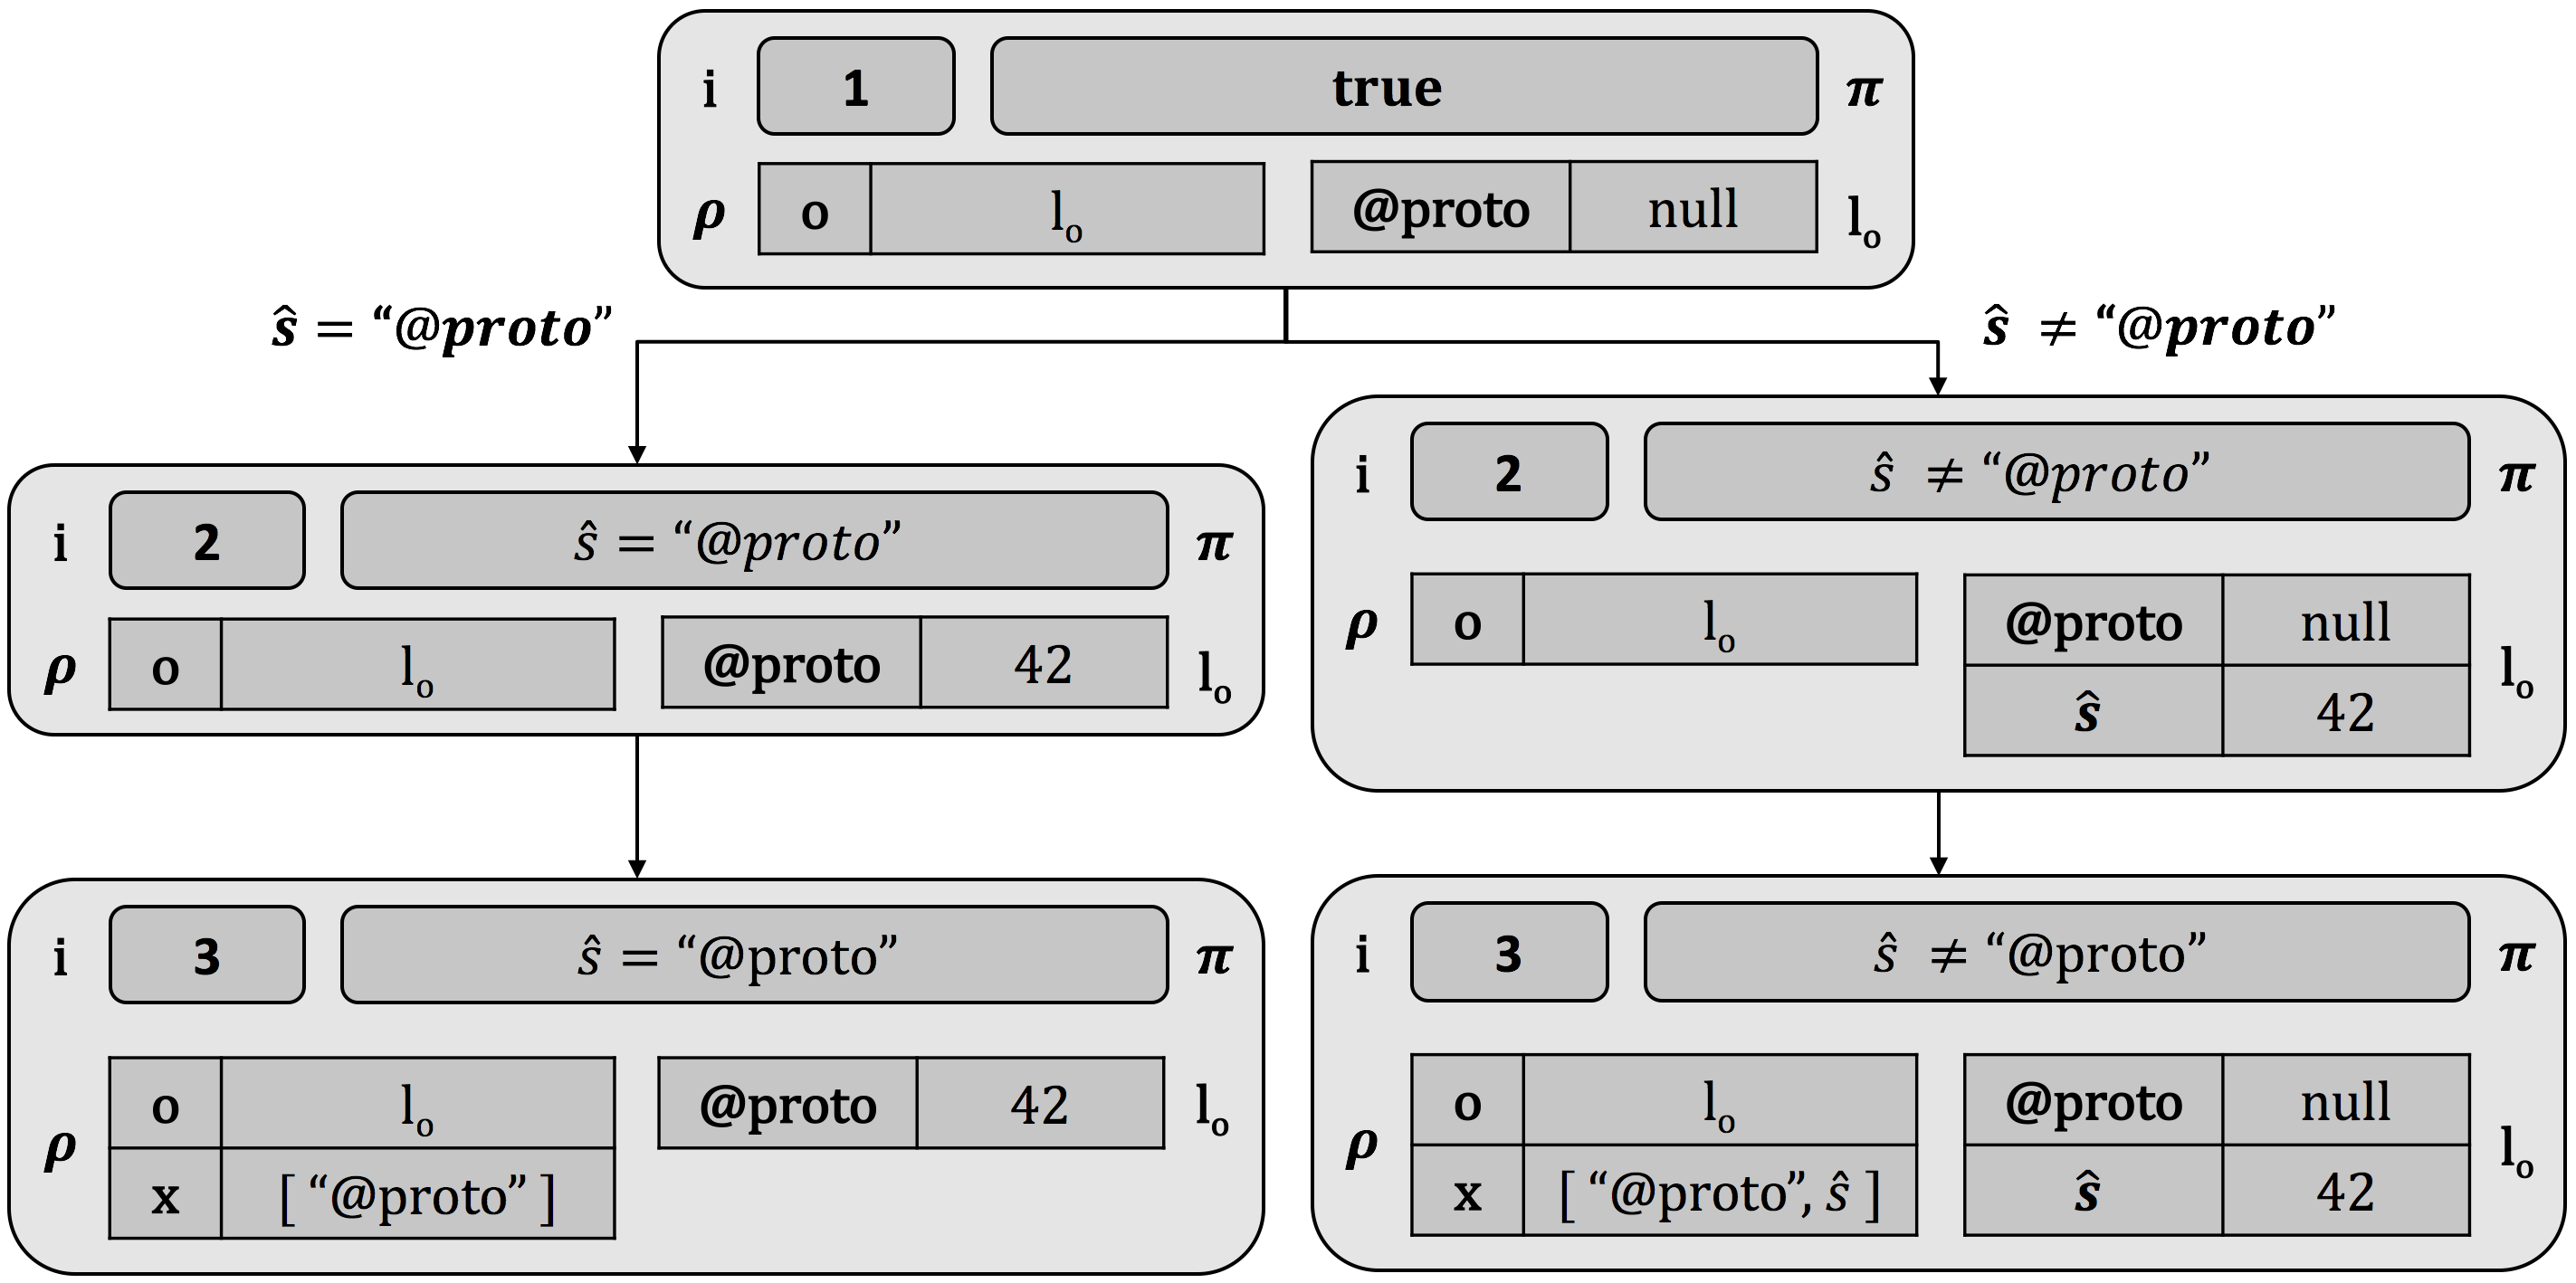
\includegraphics[width=\linewidth]{figures/symbSemEx.png}
\vspace*{-0.1cm}
\caption{Example of a \jilette symbolic execution}
\label{fig:sexecexample}
\vspace*{-0.3cm}
\end{figure}

\myparagraph{Transparency} 
Observe that a concrete state is also a symbolic state. Hence, we can feed a concrete state to the 
symbolic execution. In that case, the symbolic execution must behave exactly as the concrete 
execution. This is captured by the transparency theorem given below. 

\begin{theorem}[Transparency]\label{teo:transparency}
$\forall \, \prog, \heap, \store, i, \ctx, \mode, \heap',  \store', i',  \ctx', \mode' \, . \,$
\vspace{-5pt}
$$
  \semtranstrans[\prog][\mode][\mode']{\heap, \store, i}{\heap', \store', i'}[\ctx][\ctx']
  \iff
  \symbtranstrans[\prog][\mode][\mode']{\heap, \store, i, \jtrue}{\heap', \store', i', \jtrue}[\ctx][\ctx']. 
$$
\end{theorem}

\vspace{-5pt}
\myparagraph{Soundness} To establish the soundness of symbolic execution, we need to relate 
symbolic states to concrete states. To this end, we make use of \emph{symbolic environments} 
$\senv : \svars \rightharpoonup \vals$, mapping symbolic values to concrete values. 
A symbolic environment is \emph{well-formed} if it maps symbolic 
values to concrete values of the appropriate type (i.e.~symbolic strings are mapped to strings 
and symbolic numbers are mapped to numbers). In the following, we always 
assume well-formed symbolic environments. 
%
Given a symbolic environment $\senv$, we define the interpretation of extended expressions and symbolic expressions as follows:

\begin{figure*}[!h]
{\footnotesize
\textsc{Interpretation of Symbolic Expressions}
\vspace*{-0.1cm}
\begin{mathpar}
\semexpr{\val}{\senv} \semeq \val 
%
\qquad
%
\semexpr{\svar}{\senv} \semeq \senv(\svar)
\qquad
%
\semexpr{\unoper\ \sexpr}{\senv} \semeq \semop{\unoper} (\semexpr{\sexpr}{\senv})
\qquad 
\semexpr{\sexpr_1 \binoper \sexpr_2}{\senv} \semeq \semop{\binoper}(\semexpr{\sexpr_1}{\senv}, \semexpr{\sexpr_2}{\senv}) 
\end{mathpar}


\textsc{Interpretation of Extended Expressions}
\vspace*{-0.2cm}
\begin{mathpar}
{\begin{array}{c}
\semexpr{\val}{\senv} \semeq \val \\[2pt]
%
\semexpr{\xvar}{\senv} \semeq \xvar \\[2pt]
%
\semexpr{\svar}{\senv} \semeq \senv(\svar)
\end{array}}
\quad
%
\frac{\semexpr{\pvsexpr}{\senv} = \val}
      {\semexpr{\unoper\ \pvsexpr}{\senv} \semeq \semop{\unoper} \val}
%
\quad
%
\frac{\semexpr{\pvsexpr}{\senv} = \pvsexpr' \not\in \vals}
       {\semexpr{\unoper\ \pvsexpr}{\senv} \semeq \unoper \ \pvsexpr'}
%
\quad
\frac{ \val = \semop{\binoper}(\semexpr{\pvsexpr_1}{\senv}, \semexpr{\pvsexpr_2}{\sstore})} 
       {\semexpr{\pvsexpr_1 \binoper \pvsexpr_2}{\senv} \semeq \val}
 %
 \quad
\frac{{\begin{array}{c}
	\semexpr{\pvsexpr_1}{\senv} = \pvsexpr_1' 
	  \quad 
	  \semexpr{\pvsexpr_2}{\senv} = \pvsexpr_2'
	  \\
	  \pvsexpr_1' \not\in \vals \ \vee \ \pvsexpr_2' \not\in \vals 
	  \end{array}}
	}
	{\semexpr{\pvsexpr_1 \binoper \pvsexpr_2}{\senv} \semeq \pvsexpr_1' \, {\binoper} \, \pvsexpr_2'}
\end{mathpar}}
\vspace*{-0.4cm}
\end{figure*}

We extend this interpretation to heaps, stores, contexts, basic commands, commands, procedures, and programs in the standard way, shown in the Appendix.  
We say that a symbolic environment is \emph{consistent} with a path condition 
$\pc$, written $\senv \vdash \pc$,  if and only if $\semexpr{\pc}{\senv} = \jtrue$. 
Given a symbolic state $(\sheap, \sstore, \sctx)$ and a path condition $\pc$, we define 
the models of the symbolic state under $\pc$, written $\smodels{\sheap, \sstore, \sctx}{\pc}$, 
as the set of concrete states that can be obtained from $(\sheap, \sstore, \sctx)$ using 
symbolic environments that are consistent with~$\pc$. Formally:

{\small \begin{align}
\smodels{\sheap, \sstore, \sctx}{\pc} & = \left\{ (\heap, \store, \ctx, \senv) \mid \semexpr{(\sheap, \sstore, \sctx)}{\senv} = (\heap, \store, \ctx) \, \wedge \,  \senv \satisfies \pc  \right\} \\
\smodels{\sheap, \sstore}{\pc} & = \left\{ (\heap, \store, \senv) \mid \semexpr{\sheap}{\senv} = \heap \, \wedge \, \semexpr{\sstore}{\senv} = \store \, \wedge \,  \senv \satisfies \pc  \right\}
\end{align}}

%\begin{figure}[t!]
%{\small
%\begin{tabular}{l}
%$\quad${\bf Interpretation of Symbolic Expressions:}  \\
%$
%\quad
%\semexpr{\val}{\senv} \semeq \val
%\quad 
%\semexpr{\jvar}{\senv} \semeq \jvar
%\quad 
%\semexpr{\svar}{\senv} \semeq \senv(\svar)
%\quad 
%\semexpr{\unoper\ \sexpr}{\senv} \semeq \semop{\unoper} (\semexpr{\sexpr}{\senv})
%\quad 
%\semexpr{\sexpr_1 \binoper \sexpr_2}{\senv} \semeq \semop{\binoper}(\semexpr{\sexpr_1}{\senv}, \semexpr{\sexpr_2}{\senv}) 
%$
%\\[3pt]
%$\quad${\bf Symbolic Heaps:}  \\
%$
%\quad
% \semexpr{\hemp}{\senv} \semeq \hemp
%\quad
%\semexpr{\hcell{\loc}{\sexpr_p}{\sexpr_v}}{\senv} \semeq  \hcell{\loc}{\semexpr{\sexpr_p}{\senv}}{\semexpr{\sexpr_v}{\senv}}
%\quad
%\semexpr{\sheap_1 \dunion \sheap_2}{\senv} \semeq  \semexpr{\sheap_1}{\senv} \dunion \semexpr{\sheap_2}{\senv}
%$%
%%%
%%%
%\\[3pt]
%$\quad${\bf Symbolic Stores:}  
%$
% \semexpr{\storeemp}{\senv} \semeq \storeemp
%\quad 
% \semexpr{(\jvar: \sexpr) \dunion \sstore}{\senv} \semeq (\jvar: \semexpr{\sexpr}{\senv}) \dunion \semexpr{\sstore}{\senv}
%$%
%\\[3pt]
%$\quad${\bf Symbolic Contexts:}  
%$ \semexpr{\lstemp}{\senv} \semeq \lstemp
%\quad 
% \semexpr{(\pid, \sstore, \jvar, i, j) \lstcons \sctx}{\senv} \semeq (\pid, \semexpr{\sstore}{\senv}, \jvar, i, j) \lstcons \semexpr{\sctx}{\senv}
%$%
%
%\\[3pt]
%$\quad${\bf Symbolic States:}  $\semexpr{(\sheap, \sstore, \sctx)}{\senv} \semeq (\semexpr{\sheap}{\senv}, \semexpr{\sstore}{\senv}, \semexpr{\sctx}{\senv})$
%\end{tabular}
%}
%\caption{Interpretation of symbolic expressions, heaps, stores, and contexts.\label{fig:symbolic:interp}}
%\vspace{-0.5cm}
%\end{figure}

\vspace*{-0.3cm}
The soundness theorem (Theorem~\ref{teo:soundness:jsil:symb:exe}) states that if we have a symbolic trace captured by 
$\symbtranstrans[\prog][\mode][\mode']{\sheap, \sstore, i, \pc}{\sheap', \sstore', i', \pc'}[\sctx][\sctx']$ 
and a concrete state $(\heap, \store, \ctx)$ with a symbolic environment~$\senv$
in the models of the initial symbolic state under 
the final path condition $\pc'$, and $\senv$ concretises all symbolic variables of the program $\prog$, then there exists a concrete symbolic state $(\heap', \store', \ctx')$ 
that is in the models of the final symbolic state under $\pc'$ with the same symbolic environment~$\senv$, such that: 
$\semtranstrans[\symbeval{\prog}{\senv}][\mode][\mode']{\heap, \store, i}{\heap', \store', i'}[\ctx][\ctx']$. 
 We use the final path condition $\pc'$ for both the models of the initial and final 
symbolic states because we only care about the initial concrete states for which 
the concrete execution will follow the same path as the symbolic execution. 
%
\begin{theorem}[Soundness]\label{teo:soundness:jsil:symb:exe}
$\forall \, \prog, 
	\sheap, \sstore, i, \pc, \sctx, \mode, 
	\sheap', \sstore', i', \pc', \sctx', \mode', 
	\heap, \store, \ctx, \senv \, .$
\vspace*{-0.65cm}
$$
\begin{array}{l}
\\  
\quad \symbtranstrans[\prog][\mode][\mode']{\sheap, \sstore, i, \pc}{\sheap', \sstore', i', \pc'}[\sctx][\sctx'] 
   \ \wedge \ 
      (\heap, \store, \ctx, \senv) \in \smodels{\sheap, \sstore, \sctx}{\pc'} \\ \quad \quad
      	 \ \Rightarrow \ \exists \heap', \store', \ctx' \, . \, 
	 	 \semtranstrans[\symbeval{\prog}{\senv}][\mode][\mode']{\heap, \store, i}{\heap', \store', i'}[\ctx][\ctx']
		\, \wedge \, 
		(\heap', \store', \ctx') \in \smodels{\sheap', \sstore', \sctx'}{\pc'}  
\end{array}
$$
\end{theorem}
%
The \emph{bug-finding} corollary (Corollary~\ref{bug:finding}) states that if 
we find a symbolic trace that results in a failed assertion, 
then there also exists a concrete execution that will cause that assertion to fail.
Observe that the analysis is designed in such a way that there are no false positives, 
meaning that if we find a failing symbolic trace,
we can always instantiate its symbolic values obtaining a concrete counter-model for the 
failing assertion. This is essential, as \jilette is meant to be a \emph{bug-finding} tool.
%
\begin{corollary}[Bug-finding]\label{bug:finding}
$\forall \, \prog, \sheap, \sstore, i, \pc, \sctx, \sheap', \sstore', j, \pc', \sctx' \, .$
\vspace*{-0.2cm}
$$
\begin{array}{l} 
 \quad \symbtranstrans[\prog][\top][\bot]{\sheap, \sstore, i, \pc}{\sheap', \sstore', j, \pc'}[\sctx][\sctx']  \\ 
   \qquad \Rightarrow 
     \exists \heap, \store, \ctx, \senv \, . \, (\heap, \store, \ctx, \senv) \in \smodels{\sheap, \sstore, \sctx}{\pc'} \ \wedge \ \semtranstrans[\symbeval{\prog}{\senv}][\top][\bot]{\heap, \store, i}{\_, \_, \_}[\ctx][\_]. 
\end{array}
$$
\end{corollary}
%
Finally, the \emph{verification} corollary (Corollary~\ref{corollary:verification})
states that if we have symbolically explored all the possible execution paths
starting from a given symbolic state $(\sheap, \sstore, \sctx)$,  
then the execution of the program starting from  any concrete state in the models 
of the initial symbolic state (under the initial path condition) will result in a final concrete state
in the models of one of the final symbolic states (under its associated path condition).  
As \jilette does not infer loop invariants, if a \jsil program contains loops that cannot be unrolled statically, we will never be in the case of the verification corollary. 

\begin{corollary}[Verification]\label{corollary:verification}
$$
\begin{array}{l}
\forall \, \prog, \sheap, \sheap_1, ..., \sheap_n, \sstore, \sstore_1, ..., \sstore_n, \sctx, \sctx_1, ..., \sctx_n, i, j_1, ..., j_n, \pc, \pc_1, ..., \pc_n,\mode, \mode_1, ..., \mode_n. \\
   \;\; \wedge_{k=1}^n \left(\symbtranstrans[\prog][\mode][\mode_k]{\sheap, \sstore, i, \pc}{\sheap_k, \sstore_k, j_k, \pc_k}[\sctx][\sctx_k]\mid_{k = 1}^n\right) 
      \ \wedge \ \pc \vdash \bigvee_{k=1}^n \pc_k \\ 
       \;\;\;\; \Rightarrow \left(
         \forall \heap, \store, \ctx, \senv \, . \, (\heap, \store, \ctx, \senv) \in \smodels{\sheap, \sstore, \sctx}{\pc} \right. \\
           \;\;\;\;\;\; \left. \Rightarrow \exists k, \heap', \store', \ctx' \, . \, 
                  \semtranstrans[\symbeval{\prog}{\senv}][\mode][\mode_k]{\heap, \store, i}{\heap', \store', j_k}[\ctx][\ctx'] \ \wedge \ 
                  (\heap', \store', \ctx', \senv) \in \smodels{\sheap_k, \sstore_k, \sctx_k}{\pc_k} \right)
\end{array}
$$ 
\end{corollary}
%
The {\bf proofs} of the above results are given in the Appendix. \polish{What do these results mean with respect to related work? How is this maintainable?} 


\subsection{Implementation}
\label{subsec:jsil:analysis:implementation}

Implementing a symbolic execution engine for \jsil is a non-trivial 
task, requiring a substantial engineering effort. 
% 
% 
Hence, instead of implementing the symbolic semantics of \jsil from scratch, we leverage on 
\rosette~\cite{Rosette1,Rosette2}, a symbolic virtual machine designed to 
enable swift development of new 
solver-aided languages. 
%
\rosette is a small extension of Racket~\cite{racket} equipped with a symbolic compiler with support 
for symbolic values and first order assertions. Because \rosette is itself solver-aided, languages 
implemented in \rosette can also make use of the solver-aided facilities provided by \rosette. 
Hence, by implementing a \emph{concrete} \jsil interpreter in \rosette, we obtain \emph{for free} a symbolic 
interpreter for \jsil. %consistent with the symbolic semantics described in  \S\ref{subsec:jsil:analysis:formalism}. 
%The idea of turning a concrete interpreter into a symbolic interpreter by embedding it in 
%
The implementation of the concrete interpreter in \rosette must fulfil the following criteria:

\begin{itemize}          
   \item \emph{Efficiency:} the implementation must promote \rosette's efficient behaviour;
   
   \item \emph{Termination:} the user must be given a way to establish a bound for the symbolic execution 
            of programs that loop on symbolic values; 
  
   \item \emph{Adequacy:} the symbolic execution of the concrete interpreter in \rosette 
            must be consistent with the symbolic semantics described in \S\ref{subsec:jsil:analysis:formalism}. 
            We discuss adequacy in \S\ref{sec:evaluation} in the context of the global evaluation 
            of \jilette.
\end{itemize}

%- describe the \rosette approach to the implementation of symbolic analysis 
% - describe the encoding of \jsil concrete/symbolic states in \rosette 
% - explain the \jsil interpreter implemented in \rosette and its connection to the \jsil concrete semantics  and symbolic semantics 
%- give snippets of the interpreter 
%- discuss implementation strategies that enable \rosette to work properly

\myparagraph{Implementing \jsil in \rosette}
We first show
how to model the concrete \jsil state. Below are our \rosette encodings of \jsil heaps, stores, 
and call stacks. 
Heaps are modelled as pairs of locations and lists of property-value pairs, 
stores as lists of variable-value pairs, and call stacks as lists of lists, each of which
contains the \rosette encoding of the appropriate four elements. 
\jsil variables and function identifiers are modelled 
as Racket symbols.\footnote{Racket symbols are uninterpreted values and can be viewed as immutable strings.} 
\jsil values with \rosette correspondents are mapped accordingly; the remaining 
ones are modelled as Racket symbols (e.g. \jsil types, $\jsundefined$, $\jsnull$, and $\jsilempty$). 

The implementation of \jsil commands precisely follows their concrete semantics as 
described in \S\ref{subsec:jsil:analysis:formalism}. 
To show this, let us consider the fragment of the \jsil interpreter that implements 
the \prooflab{Property Assignment} rule, shown in Figure~\ref{rosette:interpreter:fragment}.
The figure shows three functions: \dtag{1} \schemeinline|(run-bcmd bcmd heap store)|, for 
executing basic commands, \dtag{2} \schemeinline|(update-heap heap loc prop val)|, for 
updating the heap \schemeinline|heap| by setting the value of the 
the property \schemeinline|prop| of the object denoted by \schemeinline|loc| to \schemeinline|val|, 
and \dtag{3} \schemeinline|(update-pv-list pv-list prop new-val)|,
for updating the property-value list \schemeinline|pv-list| by setting \schemeinline|prop|
to \schemeinline|new-val|.

\begin{display}{\rosette implementation of the \jsil symbolic state}
{\scriptsize
\begin{mathpar}
\inferrule[\textsc{Empty Heap}]
  {}{\roscomp{\hemp} \semeq (\racketlist)} 
\and 
\inferrule[\textsc{Non-empty Heap}]
  {
  	 \sheap_1 = \big((l, \sexprp_i) \mapsto \sexprv_i\big)\mid_{i = 0}^n   
	 \quad 
	 (\loc, -) \not\in \domain(\sheap_2)
  }{\roscomp{\sheap_1 \dunion \sheap_2} \semeq  (\racketcons (\racketcons \loc \, (\racketlist \, (\racketcons \sexprp_0 \, \sexprv_0) \cdots   (\racketcons \sexprp_n \, \sexprv_n)))  \ \roscomp{\sheap_2})} 
 \\
\inferrule[\textsc{Empty Store}]
  {}{\roscomp{\storeemp} \semeq (\racketlist)} 
\and 
\inferrule[\textsc{Non-Empty Store}]
  {}{\roscomp{(\jvar: \sexpr) \dunion \sstore} \semeq (\racketcons \, (\racketcons \, (\racketquote \jvar) \ \sexpr) \,  \roscomp{\sstore})} 
\\ 
\inferrule[\textsc{Empty Context}]
  {}{\roscomp{\lstemp} \semeq (\racketlist)} 
\quad 
\inferrule[\textsc{Non-Empty Context}]
  {}{\roscomp{(\fid, \sstore, \jvar, i, j) \lstcons \sctx} \semeq  (\racketcons \,  (\racketlist \, (\racketquote \fid) \, \roscomp{\sstore} \, (\racketquote \jvar) \, i \, j) \, \roscomp{\sctx})} 
\end{mathpar}}
\end{display}

 

\lstset{language=Scheme, numbers = left}

\begin{figure}[t!]
\centering
\begin{lstlisting}
(define (run-bcmd bcmd heap store)
  (let ((cmd-type (first bcmd)))
    (cond
    	[(eq? cmd-type 'p-assign)
      	 (let* ((loc-val  (run-expr (second bcmd) store))
                (prop-val (run-expr (third bcmd)  store))
                (rhs-val  (run-expr (fourth bcmd) store)))
            (cons (update-heap heap loc-val prop-val rhs-val) store))]
         ...)))
\end{lstlisting}

\begin{lstlisting}
(define (update-heap heap loc prop val)
  (cond
    [(null? heap) (error "Inexistent object")]
    [(equal? (caar heap) loc)
       (cons (cons loc (update-pv-list (cdar heap) prop val)) (cdr heap))]
    [ else (cons (car heap) (update-heap (cdr heap) loc prop val))]))
\end{lstlisting}

\begin{lstlisting}         
(define (update-pv-list pv-list prop new-val)
  (cond
    [(null? pv-list) (list (cons prop new-val))]
    [(equal? (caar pv-list) prop) (cons (cons prop new-val) (cdr pv-list))]
    [ else (cons (car pv-list) (update-pv-list (cdr pv-list) prop new-val))]))
\end{lstlisting}
\vspace*{-0.3cm}
\caption{Fragment of the \jsil Interpreter in \rosette\label{rosette:interpreter:fragment}}
\vspace*{-0.5cm}
\end{figure}

\jsil commands are represented in \rosette as \emph{s-expressions}. 
 For instance, the property assignment basic command $[\jsilexpr_1, \jsilexpr_2] := \jsilexpr_3$
 is represented as: 

\vspace*{-0.2cm}
{\small $$
\mathtt{(list \ (quote\ {p\text{--}assign}) \ \roscomp{\jsilexpr_1} \ \roscomp{\jsilexpr_2} \ \roscomp{\jsilexpr_3})}
$$}
\vspace*{-0.4cm}

\noindent Therefore, the interpreter of basic commands first checks if the first element of the 
list representing the command is equal to \schemeinline|p-assign|. If it is, 
it uses the function \schemeinline|run-expr| to evaluate the three \jsil expressions 
comprising the property-assignment in the appropriate order. Then, it invokes the 
function \schemeinline|update-heap| to perform the actual update. 
The function \schemeinline|update-heap| recursively iterates over all heap objects
to find the object whose property is to be updated and, when it finds it, 
uses the function \schemeinline|update-pv-list| to update the corresponding 
field-value list. If it does not find it, it will raise an error. However, due to the concrete semantics of \jsil, this case is never triggered.

\lstset{language=Scheme, numbers=none, backgroundcolor=\color{mygray}}
\myparagraph{Efficiency}
It is often possible for more than one transition of the symbolic 
semantics to be applicable during symbolic execution, 
giving rise to a potentially intractable number of possible symbolic states. 
To counter this problem, \rosette uses a sophisticated 
symbolic state merging algorithm, which factors out the common 
part between multiple symbolic states  in order to expose more 
opportunities for concrete evaluation. The non-mergeable portions of the state 
are represented as \emph{guarded symbolic unions}. 
Our goal is to write the interpreter code in a way that helps 
\rosette merge sets of possible symbolic states, yielding minimal 
guarded symbolic unions.
To illustrate this point, let us consider the symbolic execution 
of the property assignment $\mathtt{o[\hat{s}] := 42}$ in the 
symbolic heap represented in \rosette as follows: 

\smallskip
\noindent
\begin{BVerbatim}[fontsize=\footnotesize,commandchars=\$\{\},bgcolor=Gainsboro]
(lo (("@proto" null) ("a" 0) ("b" 1))) $phantom{xxxxxxxxxxxxxxxxxxxxxxxxxxxxxxxxxxxxxxxxxxxxxxxxx}
\end{BVerbatim}

\smallskip
\noindent
with a symbolic store mapping \schemeinline|o| to \schemeinline|lo| and 
the path condition {\small $\mathtt{\hat{s} = \text{\texttt{"a"}} \ \vee \hat{s} = \text{\texttt{"b"}}}$}.
The two resulting symbolic heaps are represented in \rosette as:  

\smallskip
\noindent
\begin{BVerbatim}[fontsize=\footnotesize,commandchars=\$\{\},bgcolor=Gainsboro]
(lo (("@proto" null) ("a" (? (= $shat "a") 42 0)) ("b" (? (= $shat "b") 42 1))) $phantom{xxxxxxxxxxxxxxxx}
\end{BVerbatim}

\smallskip
\noindent
Here, \rosette manages to push the guarded unions to 
the object cells that may be affected by the property assignment, maintaining a common 
property-value list for both resulting symbolic states. 
Now, let us change the code of line 6 of \schemeinline|update-pv-list| 
(in Figure~\ref{rosette:interpreter:fragment}) to:  

\smallskip
\noindent
\begin{BVerbatim}[fontsize=\footnotesize,commandchars=\$\{\},bgcolor=Gainsboro]
(append (cdr pv-list) (cons prop new-val)) $phantom{xxxxxxxxxxxxxxxxxxxxxxxxxxxxxxxxxxxxxxxxxxxxx}
\end{BVerbatim}

\smallskip
\noindent
This change in the interpreter makes the order of the cells in the property-value 
list change depending on which property gets updated. 
Now, \rosette needs to create a single guarded union 
with the two possible resulting property-value lists: 

\smallskip
\noindent
\begin{BVerbatim}[fontsize=\footnotesize,commandchars=\$\{\},bgcolor=Gainsboro]
(lo (? (= $shat "a") (("@proto" null) ("b" 1) ("a" 42)) (("@proto" null) ("a" 0) ("b" 42)))) 
\end{BVerbatim}

\myparagraph{Termination} The \jsil symbolic execution engine does not 
include the abstraction mechanisms which would allow it to finitise the symbolic 
execution of loops depending on symbolic values~\cite{abstract:symbolic:exec}. 
Hence, the user is asked to specify an upper bound on the number of times
the symbolic execution is allowed to branch on symbolic values by using
conditional gotos. 
Once that upper bound is reached, if a conditional goto that branches 
on a symbolic value is encountered, the symbolic execution stops.  

%
%\myparagraph{Adequacy} 
%We strongly believe that the symbolic execution of the concrete interpreter 
%in \rosette is consistent with respect to the \jsil symbolic semantics. 
%In fact, we have ``reverse-engineered'' our \jsil symbolic execution by 
%observing in detail the guarded unions produced by Rosette for each of 
%the \jsil commands. Due to its complexity and scale, 
%{a formal proof would require
%mechanisation}, which is, unfortunately, beyond our manpower.
 
%Hence, the user is asked to specify an upper bound on the number of times
%the symbolic execution is allowed to branch depending on symbolic values. 
%Once that upper bound is reached, if a conditional goto that branches 
%on a symbolic value is encountered, the symbolic execution simply stops.  

\lstset{backgroundcolor=\color{white}}

\section{Symbolic Testing for JavaScript}
\label{sec:sym:exec:js}

\begin{figure}[h]
%\vspace*{-0.4cm}
\centering
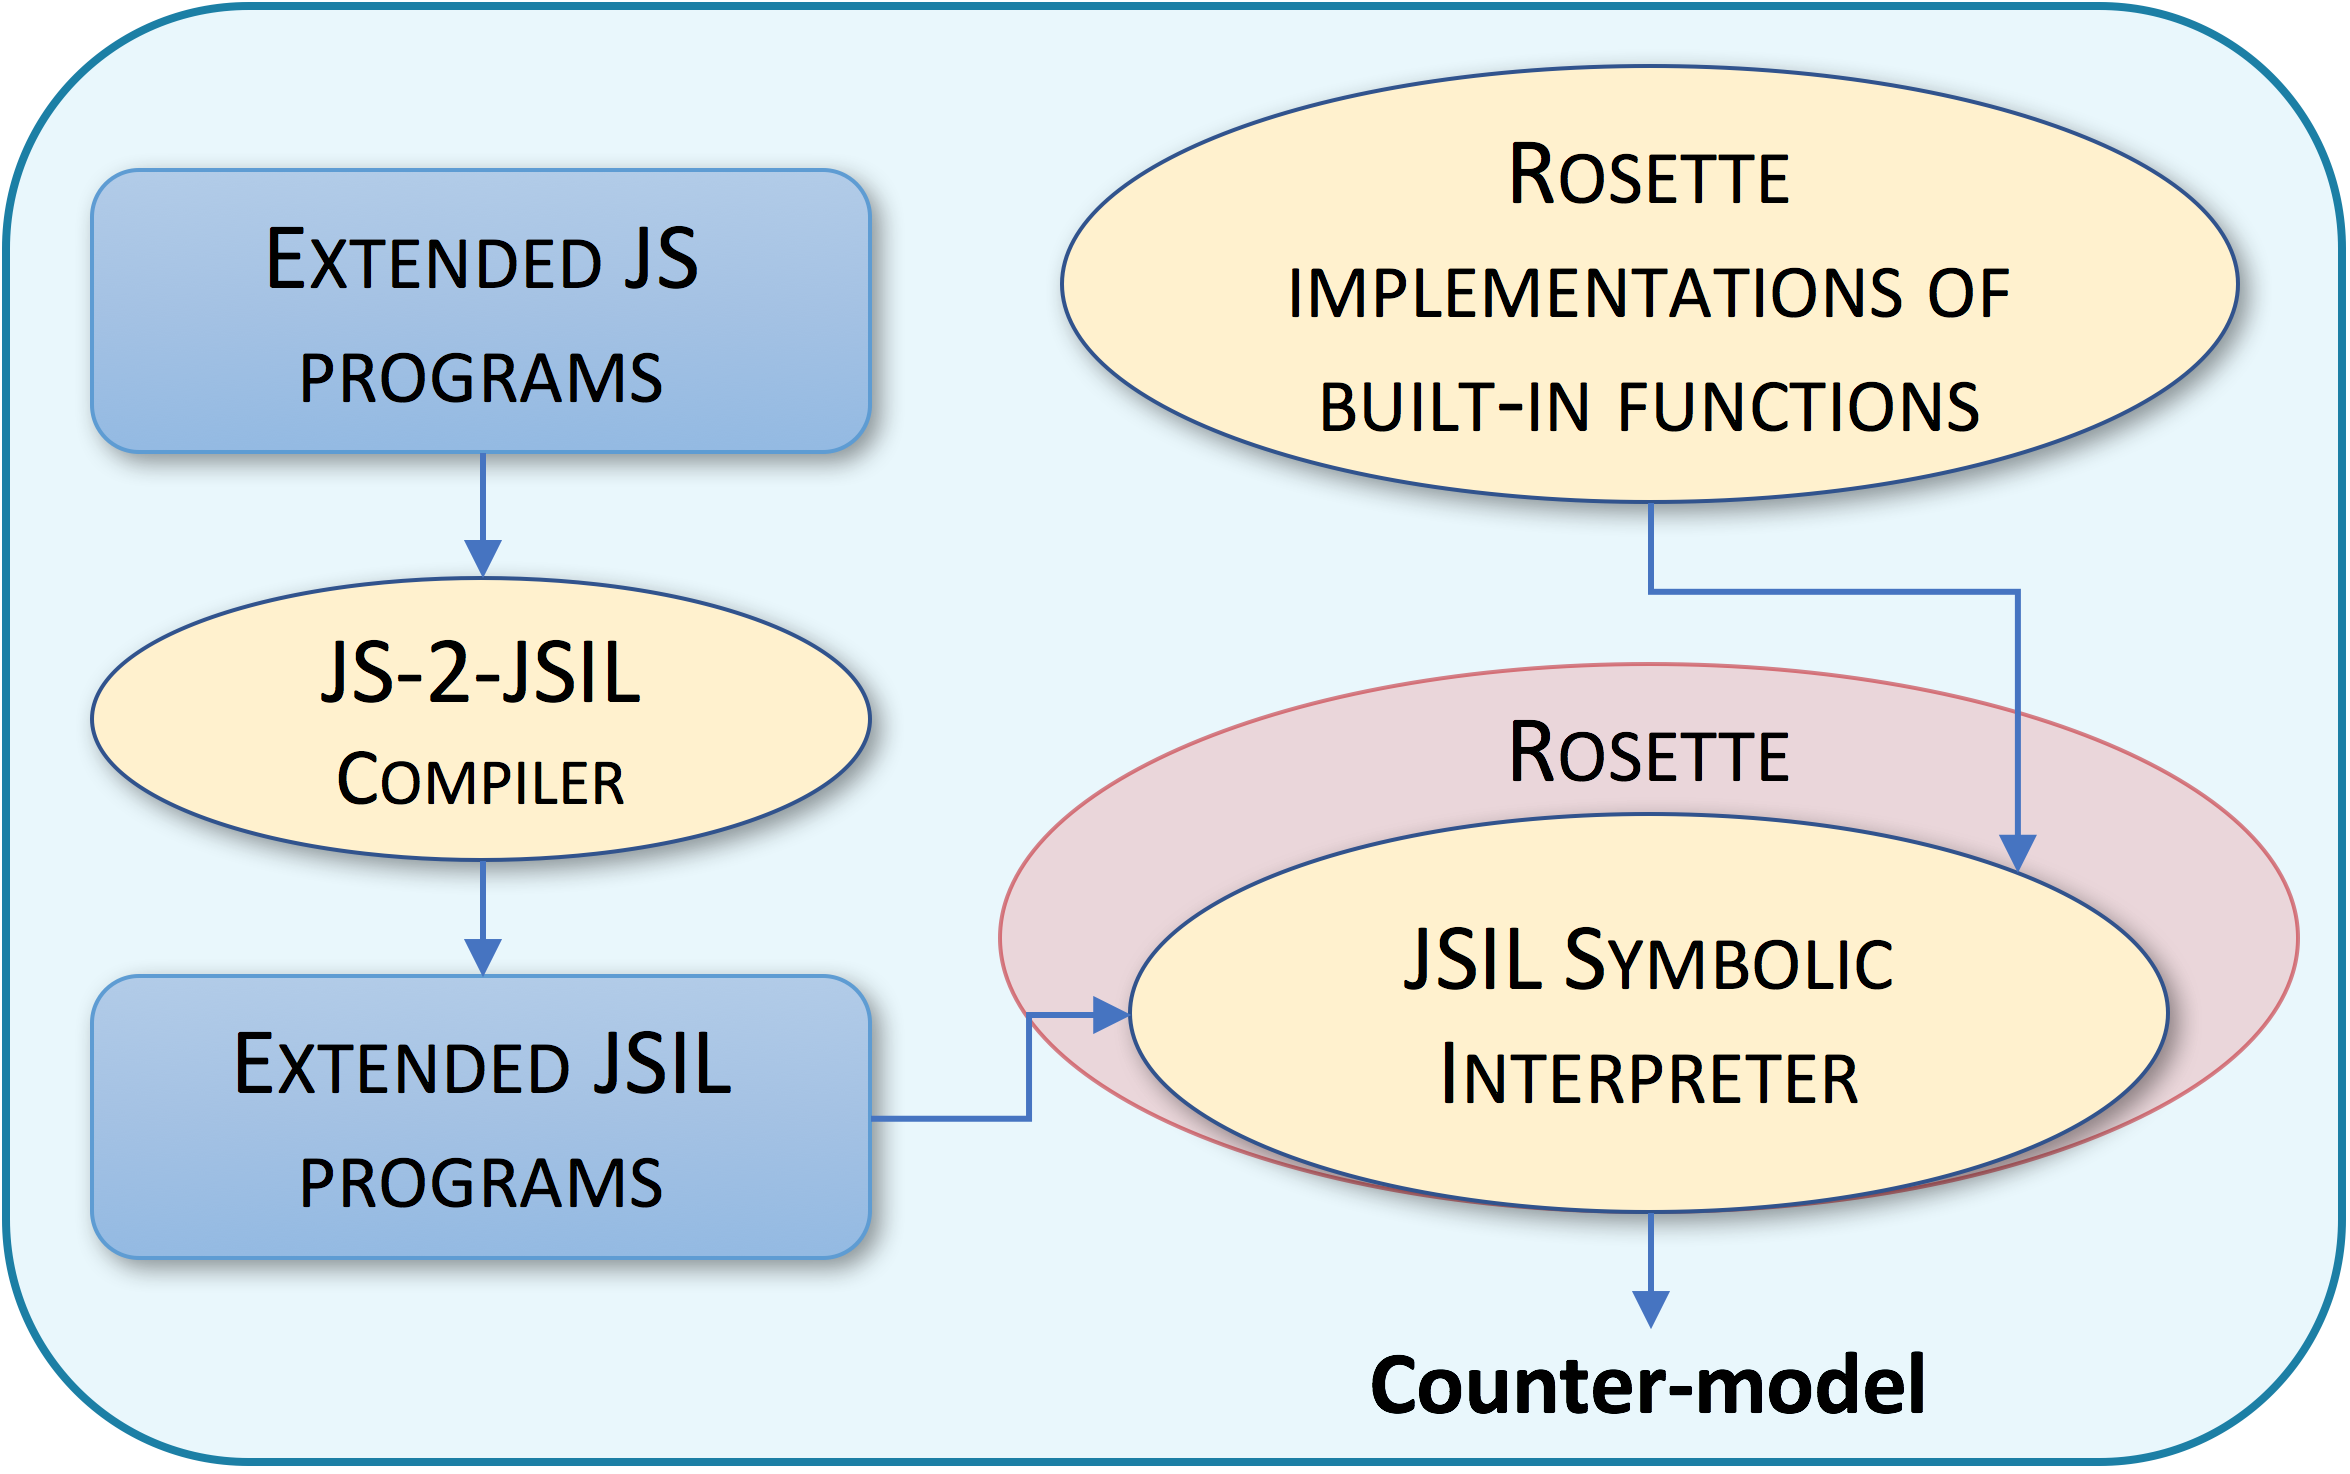
\includegraphics[width=\linewidth]{figures/jilette_blue.png}
%\vspace*{-0.2cm}
\caption{\jilette: Symbolic execution for JavaScript}
%\vspace*{-0.3cm}
\label{fig:jilette:diagram}
\end{figure}

Symbolic execution designed directly on JavaScript is not feasible, for the same reasons verification is not~\cite{JoseCADE}: the semantics of the language is too complex, with numerous intertwined internal functions called under the hood. 
In particular, the simple assignment alone would have more than twenty potential branchings. 
Our approach is to symbolically analyse JavaScript code by first compiling it to \jsil, using~\JSComp~\cite{javert}, and then feeding the compiled \jsil code to our \jsil symbolic interpreter, described in \S\ref{sec:jsil:symb:exec}.

In \S\ref{symb:exec:comp}, we explain how we enable symbolic execution for JavaScript using \JSComp and Rosette, by extending the language with new constructs for the creation of symbolic values and the checking of assertions.
Next, in \S\ref{symbolic:testing}, we explain how this symbolic execution can be used for systematic symbolic testing of JavaScript code. 
Finally, in \S\ref{builtins}, we present
a general approach for streamlined symbolic execution of JavaScript built-in libraries, which maximises the use of Rosette's native solver-aided facilities.

%More concretely, we extend the \jsil symbolic interpreter with \rosette implementations of JavaScript built-in libraries in a streamlined manner.  
%These implementations are both an easy way to get a better coverage of the standard and 
%match the abstraction level of the generated JSIL code precisely with the abstraction level 
%of Rosette, maximising the use of Rosette's native solver-aided facilities.

%to make sure that we make proper use of theof \rosette.    

\subsection{Symbolic Execution by Compilation} 
\label{symb:exec:comp}

\myparagraph{Extending JavaScript Syntax}
We extend the syntax of JavaScript with logical expressions $\jslexpr$, 
and the following constructs: %(corresponding to JavaScript normal expressions): 
\dtag{1} $\jsassert(\jslexpr)$, stating that whenever the \emph{assert} is reached, 
$\jslexpr$ must evaluate to $\jtrue$; 
\dtag{2} $\jsassume(\jslexpr)$, stating that we \emph{assume} $\jslexpr$ to hold along the
current program path; 
\dtag{3} $\jssymbstring()$, for creating a fresh symbolic string; and
\dtag{4} $\jssymbnumber()$, for creating a fresh symbolic number. 
The \emph{assert} and \emph{assume} constructs expect as an argument 
a logical expression. 
Logical expressions $\jslexpr$ are given by the grammar 
$\jslexpr \triangleq \jslit \mid \jsvar \mid \unoper\ \jslexpr \mid \jslexpr \binoper \jslexpr$, 
where $\jslit$ ranges over JavaScript literal values (numbers, booleans, strings, \jsinline|undefined|, and \jsinline|null|), $\jsvar$ over JavaScript variables, 
$\unoper$ over the \jsil unary operators, and $\binoper$ over the \jsil binary operators.
Note that the JavaScript binary and unary operators may have side effects; furthermore,  
the semantics of these operators often includes several implicit type coercions 
performed in a specific (and counter-intuitive) order. 
Hence, we do not allow arbitrary JavaScript expressions (using JavaScript 
binary and unary operators) as the arguments for the \emph{assume} and 
the \emph{assert} constructs. Instead, we use the \jsil unary and binary operators, which have a very clear and simple semantics, without coercions or side-effects.

\myparagraph{Extending \JSComp}
Instead of giving a formal semantics for the newly introduced constructs, we explain 
their meaning by showing their compilation to \jsil. 
Importantly, the JavaScript variable store is emulated in the heap. 
Hence, a JavaScript variable $\jsvar$ is not compiled to a \jsil variable $\jvar$, but to a sequence  
of \jsil commands for retrieving the value of $\jsvar$ from the heap cell in which it is stored. 
A full description of \JSComp is out of the scope of this paper; see~\cite{Daiva2017}
for further details.
%
In the following, we will assume to have a function $\compile : \jstmts \rightharpoonup \lists(\cmds) * \jvars$, mapping JavaScript expressions 
and statements to lists of \jsil commands paired up with \jsil variables. 
In a nutshell, $\compile(\jstmt) = ([ \jcmd_1, ..., \jcmd_n], \jvar)$ means that the compilation 
of the JavaScript statement $\jstmt$ results in the list of \jsil commands $[ \jcmd_1, ..., \jcmd_n]$, 
and that after the execution of these commands, the value to which $\jstmt$ evaluates in the 
JavaScript semantics is stored in the \jsil variable $\jvar$. 
%
Below we show the extension of $\compile$ for the constructs introduced above. 
The definition of $\compile$ relies on an auxiliary compiler $\compilel : \jlexprs \rightharpoonup \lists(\cmds) * \exprs$, 
for translating JavaScript logical expressions.

\begin{display}{Extension $\compile : \jstmts \rightharpoonup \lists(\cmds) * \jvars$ and $\compilel : \jlexprs \rightharpoonup \lists(\cmds) * \exprs$}
{\scriptsize
\begin{mathpar}
\inferrule[\textsc{Assume}]
  {
     \compilel(\jslexpr) = [\jcmd_1, ..., \jcmd_n], \jsilexpr
     \and 
     \jvar' \text{ fresh} 
     \\\\ 
     \jcmd_{n+1} = \jvar' := \jsilempty 
     \quad
     \jcmd_{n+2} = \assume(\jsilexpr) 
  }{\compile(\jsassume(\jslexpr)) \semeq [\jcmd_1, ..., \jcmd_n, \jcmd_{n+1}, \jcmd_{n+2}], \jvar'} 
\and
\inferrule[\textsc{Assert}]
  {
     \compilel(\jslexpr) = [\jcmd_1, ..., \jcmd_n], \jsilexpr
     \and 
     \jvar' \text{ fresh} 
     \\\\ 
     \jcmd_{n+1} = \jvar' := \jsilempty 
     \quad
     \jcmd_{n+2} = \assert(\jsilexpr) 
  }{\compile(\jsassert(\jslexpr)) \semeq [\jcmd_1, ..., \jcmd_n, \jcmd_{n+1}, \jcmd_{n+2}], \jvar'}
  %
  \\
  %
  \inferrule[\textsc{Symbolic String}]
  {
    \sstring \text{ fresh} 
    \and 
    \jvar \text{ fresh}
  }{\compile(\jssymbstring()) \semeq [ \jvar := \sstring ], \jvar}   
  %
  \and
  %
  \inferrule[\textsc{Symbolic Number}]
  {
    \snumber \text{ fresh} 
    \and 
    \jvar \text{ fresh}
  }{\compile(\jssymbnumber()) \semeq [ \jvar := \snumber ], \jvar}    
   %
  \and
  %
  \inferrule[\textsc{Literal}]
  {}{\compilel(\jslit) \semeq [], \jslit}   
  %
 \and
  %
  \inferrule[\textsc{JS Var}]
  {
     \compile(\jsvar) = [ \jcmd_1, ..., \jcmd_n ], \jvar
  }{\compilel(\jsvar) \semeq [ \jcmd_1, ..., \jcmd_n ], \jvar }    
   %
  \\
  %
  \inferrule[\textsc{Unary Operator}]
  {
     \compilel(\jslexpr) = [ \jcmd_1, ..., \jcmd_n ], \jvar
  }{\compilel(\unoper\ \jslexpr) \semeq [ \jcmd_1, ..., \jcmd_n ], \unoper\ \jvar }     
   %
  \and
  %
  \inferrule[\textsc{Binary Operator}]
  {
     \compilel(\jslexpr_1) = [ \jcmd_1, ..., \jcmd_n ], \jvar_1 
     \quad
     \compilel(\jslexpr_2) = [ \jcmd_1', ..., \jcmd_n'], \jvar_2
  }{\compilel(\jslexpr \binoper \jslexpr) \semeq [ \jcmd_1, ..., \jcmd_n, \jcmd_1', ..., \jcmd_n' ], \jvar_1\binoper \jvar_2 }     
\end{mathpar}}
\end{display}


\vspace*{-0.4cm}
\subsection{Symbolic Testing by Example} 
\label{symbolic:testing}

\lstnewenvironment{lstjsex}{\lstset{language=JavaScript,basicstyle=\fontsize{8}{8}\ttfamily,escapeinside={~}{~}, numbers=none, backgroundcolor=\color{mygray}}}{}

We illustrate how \jilette can be used to write symbolic tests for JavaScript code by using the JavaScript implementation 
of a  \emph{key-value map} given in Figure~\ref{map:example}~(left). 
This implementation contains four functions: 
\jsinline|Map|, for constructing an empty map;
\jsinline|get|, for retrieving the value associated with the key given as input;
\jsinline|put|, for inserting a new \emph{key-value pair} into the map and updating the values of existing keys; and
\jsinline|validKey|, for deciding whether a key is valid.

\myparagraph{Prototype chains and $\mathtt{Object.prototype}$}
In order to better understand the implementation of the map library as well as its possible bugs, 
one must first understand the \emph{prototype-based inheritance} mechanism of JavaScript. 
Every JavaScript object has a prototype, which (for presentation purposes) we assume to 
be stored  in an internal property \jsinline|@proto|. In order to determine the value of a property
\jsinline|p| of an object \jsinline|o|, the semantics first checks if \jsinline|o| has a 
property named \jsinline|p|, in which case the property look-up yields its value. Otherwise, the 
semantics checks if \jsinline|p| belongs to the properties of the prototype of \jsinline|o| and so 
forth. Hence, in the example, when looking up the value of the property \jsinline|hasOwnProperty|
of the object \jsinline|contents|, one gets the value associated with the property  \jsinline|hasOwnProperty|
of its prototype.
The sequence of objects that can be accessed from a given object through the inspection 
of the respective prototypes is called a \emph{prototype chain}.
Prototype chains typically finish with the object \jsinline|Object.prototype| from which JavaScript 
programs can access a number of built-in functions, which are part of the language runtime environment and are used for inspecting and manipulating objects.
An example of such a function is \jsinline|hasOwnProperty(p)|, which checks whether or not the object 
on which it is invoked has the property \jsinline|p| (e.g. {\small \jsinline|map.hasOwnProperty("_contents")|}
evaluates to \jsinline|true| when evaluated in the heap shown in Fig.~\ref{map:example}-(right), 
because the object \jsinline|map| has a property named~\jsinline|"_contents"|). 

 \begin{figure}[t!]
 \begin{subfigure}{\linewidth}
 \begin{lstjs}[firstnumber=1]
function Map () { this._contents = {} }

Map.prototype.get = function (k) {
  var c = this._contents;
  if (c.hasOwnProperty(k)) {
    return this._contents[k] 
  } else { return null }
}

Map.prototype.put = function (k, v) {
  var c = this._contents;
  if this._contents.validKey(k)) {  
    contents[k] = v   
  } else
    throw new Error("Invalid Key");
} 

Map.prototype.validKey = function (k) { ... }
\end{lstjs}
\caption{JS map implementation}
\end{subfigure}

\begin{subfigure}{\linewidth}
%\vspace*{-0.3cm}
%\hspace*{-1.2cm}
\centering
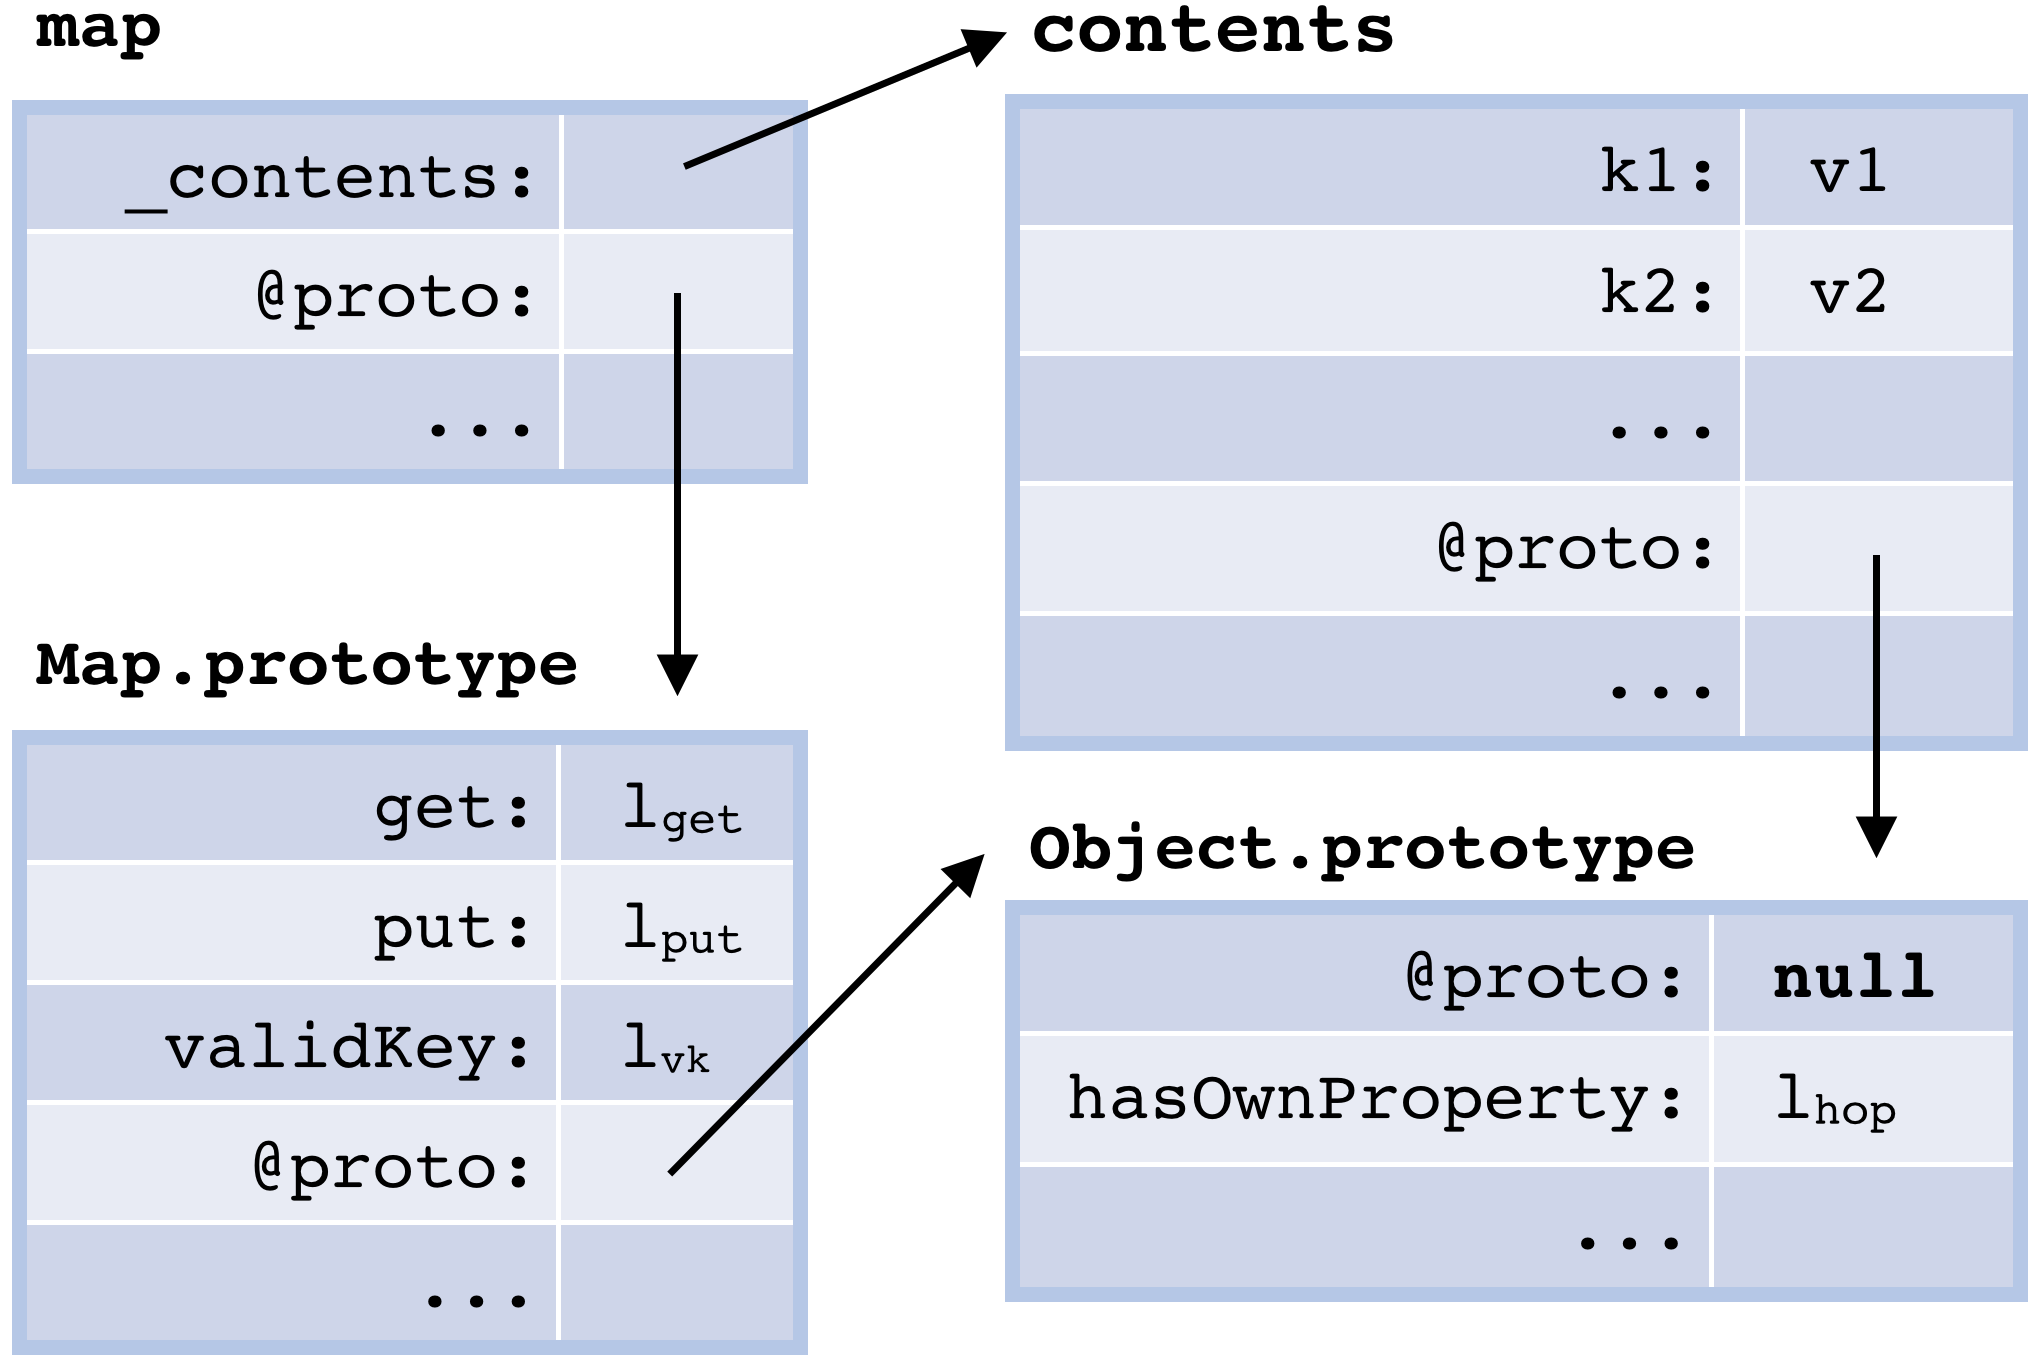
\includegraphics[width=0.8\textwidth]{figures/mapDiagram.png}
\caption{Example heap for the map library}
\end{subfigure}
%\vspace*{-0.3cm}
\caption{JS map implementation (top) and example of a map library heap (bottom) \label{map:example}}
%\vspace*{-0.5cm}
\end{figure}

\myparagraph{Bugfinding}
The map library implements a \emph{key-value map} as an object with property \jsinline|_contents|, denoting the object storing the map contents.  
The named properties of \jsinline|_contents| and their value attributes correspond to the map keys and values, respectively.
The functions \jsinline|get|, \jsinline|put|, and \jsinline|validKey| are to be shared between all map 
objects. Therefore, they are defined in \jsinline|Map.prototype|, which is the prototype 
of all objects created using \jsinline|Map| as a constructor (i.e.~using~\jsinline|new Map()|). 
%
Note that one can insert a key-value pair with \jsinline|"hasOwnProperty"| as a key into the map. 
By doing this, \jsinline|"hasOwnProperty"| in the prototype chain of
\jsinline|_contents| is overridden and subsequent calls to \jsinline|get| will fail. 
Consider the following symbolic test:
\begin{lstjsex}
var s1 = __s(); var n1 = __n(); 
var m = new Map();  m.put(s1, n1); var r = m.get(s1);  
assert(n1 = r)
\end{lstjsex}
%
The symbolic test above checks for a desired property of the library---if we were to put a key/value pair \jsinline|(k, v)| into the map, then we should be able to retrieve the value \jsinline|v| using the key \jsinline|k|. We can run \jilette on this test to reveal the bug discusses above. Indeed, \jilette generates
the failing model: \jsinline|s1 = "hasOwnProperty"|. 

This example also highlights how \jilette does not require 
specialist knowledge, and can, therefore, be used by almost any JavaScript developer. 
The annotation burden amounts to the creation of symbolic variables and the writing of assertions, remaining minimal and intuitive, in stark contrast with the standard annotation 
burden of verification tools.

%- Extensible Interpreter 
% - an easy way to have more coverage 
% - match the abstraction level of the generated code to the abstraction level of \rosette 

\subsection{Supporting JavaScript Built-in Libraries}
\label{builtins}

JavaScript comes equipped with a rich runtime environment (described in Chapter 15 of the 
ES5 standard~\cite{ecma}), which consists of \emph{built-in libraries} that support advanced manipulation of, for example, objects, arrays, strings, regular expressions, and dates. 
In this section, we identify two important challenges related to supporting the symbolic execution of
JavaScript programs that interact with built-in libraries and explain how we solve them in \jilette. 

\JSComp models built-in library functions as \jsil procedures, which can be called from within the compiled JavaScript code. However, the current runtime environment of \JSComp does not support all built-in libraries described in the standard. In particular, it doesn't support regular expressions, parts of the String library that use regular expressions, parts of the Date library, and JSON objects. The partiality of \JSComp when it comes to supporting JavaScript built-in libraries 
gives rise to the first challenge:  
\begin{quote}
\emph{Challenge 1:} \jilette should allow for modular addition of  
implementations of built-in libraries not yet covered by \JSComp.  
\end{quote}

Most JavaScript library functions are described in the language standard in terms of 
more elementary operations. For instance, operations on strings are often described in terms 
of operations on the characters that comprise the string, and often involve loops (c.f. \jsinline|String.lastIndexOf|, Ch.15.5.4.8~\cite{ecma}).
The \jsil implementations of the JavaScript built-in libraries follow the standard line-by-line, emphasising full adherence to the language standard. 
However, for some of these built-in library functions, direct \rosette correspondents exist. 
%
In such cases, we argue that these correspondents should be used instead of the 
functions provided by \JSComp, to minimise potential branching and looping on symbolic values. 
Hence, we state the second challenge as follows: 
\begin{quote}
\emph{Challenge 2:} \jilette should prioritise native \rosette operations
to the operations provided by \JSComp in the cases in which the native \rosette
operations and JavaScript operations exactly match.
\end{quote}

\myparagraph{\rosette models of JavaScript built-in functions}
To solve these two challenges, \jilette supports the on-the-fly extension of the \jsil interpreter 
with \rosette implementations of JavaScript built-in functions, which we call \rosette \emph{models}. 
Hence, every time the interpreter evaluates a procedure call, it first checks whether or 
not it corresponds to a built-in function for which there is a \rosette model. If it does, 
instead of executing the standard procedure call rule, the interpreter will instead 
execute the appropriate \rosette model. 

Below, we show a simplified \rosette model for the built-in \jsinline|String.prototype.replace|
function~(see Ch.15.5.4.11~\cite{ecma}).
This model uses the natively supported function \schemeinline|string-replace|, 
 taking advantage of \rosette reasoning capabilities.
This example illustrates an important point about the difference between JavaScript and
\rosette operations: \schemeinline|string-replace| works only with strings, but \jsinline|String.|\jsinline|prototype. |\jsinline|replace| can take arguments of any type that then get coerced to strings. Since \JSComp does not have an implementation of \jsinline|String.replace|, the \rosette model will report an error if it receives non-string arguments.
\lstset{language=Scheme, numbers=none, backgroundcolor=\color{mygray}}
\begin{lstlisting}
(define (replace str from to)
  (if (and (string? str) (string? from) (string? to))
      (list (quote normal) (string-replace str from to #:all? #f))
      (error "Unsupported call to String.prototype.replace")))
\end{lstlisting}

\myparagraph{Bug-finding with strings}
By using the appropriate \rosette models for string operations, \jilette can find bugs in  
non-trivial JavaScript programs that manipulate strings. For instance, consider 
the following naive JavaScript implementation of a string sanitiser meant to remove 
all occurrences of \emph{script tags} inside untrusted strings (for instance, those coming 
from user input or untrusted servers).
To this end, the programmer chooses to 
replace all occurrences of the string \jsinline|"script"| in the string given 
as input with \jsinline|"s"|. 
\begin{lstjsex}
function sanitise (str) { return str.replace("script", "s") }
\end{lstjsex}
Now, we can use \jilette to test if the sanitiser meets its purpose, that is, that all
strings, after being sanitised, do not contain the substring \jsinline|"script"|:
\begin{lstjsex}
var s = sanitise(__s()); 
var x = ! (s.contains("script")); d
assert(x) 
\end{lstjsex}
\jilette will, in fact, be able to come up with a counter-model for this assertion. Concretely, this counter-model is \jsinline|s1 = "scriptcript"|. Despite its simplicity, this example illustrates the complexities underpinning the 
design and implementation of robust string sanitisers, a commonly  
used defense mechanism against XSS attacks~\cite{song}. 
 
 

 
 

%Furthermore, the \jsil language itself does not feature regular expressions or native arrays, 
%and has very few operators on strings. 
%This means that, for instance, more advanced operations on strings (such as 
%\jsinline|lastIndexOf|) need to be implemented as loops over the characters that comprise 
%the string. 
%








\section{OLD -- Debugging Separation Logic Specifications}\label{sec:specs}
%!TEX root = ../main.tex

We show how to use \cosette for debugging JavaScript code annotated with 
separation logic (SL) specifications. Tools that allow for SL-reasoning about
functional correctness properties in general, and those targeting 
JavaScript in particular, require of the user to have substantial expertise 
and to go through a long and complex proof trace in order to find the precise 
source of an error. \cosette substantially simplifies this process by providing
concrete counter-models that invalidate the specification.
In \S\ref{subsec:sep:assertions}, we extend the 
 \jsil symbolic interpreter with a mechanism for asserting
SL-assertions. 
In \S\ref{subsec:countermodels}, we show how to implement this mechanism by giving a sound decision procedure for finding counter-models 
for SL-assertions.
In \S\ref{specs:to:symbolic:tests}, we present an algorithm  
for generating symbolic tests from SL-specifications, which guarantees 
that if a symbolic test fails, then Cosette must produce a concrete 
counter-model that invalidates 
the specification. Finally, in~\S\ref{specs:example}, we show how to use the 
proposed methodology for debugging JaVerT specifications~\cite{javert} of JavaScript~code. 

\subsection{\jsil Symbolic Execution with Separation Logic Assertions}
\label{subsec:sep:assertions}

We extend \jsil with a special construct, $\sepassert(P)$, for stating that 
the separation logic assertion $P$ must hold whenever $\sepassert(P)$ is evaluated. 
We use the assertion language of~\cite{javert}, with the following adaptation:
instead of \emph{untyped logical variables}, we 
use \emph{typed logical variables}, $\svar \in \svars$, which include 
symbolic numbers, $\snumber \in \snumbers$, strings $\sstring \in \sstrings$, 
and locations,~$\sloc \in \slocs$. 

\myparagraph{\jsil assertions: syntax and semantics}
\jsil assertions include: boolean operations; first-order connectives; the separating conjunction; 
existential quantification; and assertions for describing heaps. The $\lemp$ assertion describes 
an empty heap. The cell assertion, $(\lexpr_1,\lexpr_2) \pointsto \lexpr_3$,  describes an object 
at the location denoted by $\lexpr_1$ with a property denoted by $\lexpr_2$ that has the value 
denoted by $\lexpr_3$. The assertion $\emptyfields{\lexpr_1}{\lexpr_2}$ states that the object at 
the location denoted by $\lexpr_1$ has no properties other than possibly those included in the
set denoted by $\lexpr_2$. 
%
As in~\cite{gardner:popl:2012,javert}, in order to define the semantics of assertions, 
we resort to \emph{instrumented heaps} $\iheap \in \iheaps$, which differ from 
concrete heaps in that they may map object properties to the special value $\none$, 
explicitly indicating that the property does not exist (e.g. $\iheap(\loc, \jstring) = \none$
means that the object at location $\loc$ in the heap $\iheap$ does not have a property
named~$\jstring$). 
%Analogously, we extend symbolic heaps with $\none$-cells, obtained \emph{instrumented symbolic heaps} $\isheap \in \isheaps$. 
Instrumented heaps are related to heaps by means of an \emph{erasure 
function}, $\deabstract{.}: \iheaps \rightarrow \heaps$, %($\deabstract{.}: \isheaps \rightarrow \sheaps$), 
which simply removes the none-cells from the instrumented heap given as input.  Below, we give the syntax and semantics of \jsil assertions. Note that we assume pure assertions to have an empty spatial footprint and allow logical negation, conjunction, and disjunction of pure formulae only.

%  \deabstract{\jsilaheap}(\loc, x) = \jsilaheap(\loc, x) \iffdef (\loc, x) \in \domain(\jsilaheap) \ \wedge \ \jsilaheap(\loc, x) \neq \none

\begin{display}{\jsil Logic Assertions - Syntax and Semantics}
%
{\scriptsize \begin{tabular}{lll}
  %%%% 
  $\quad \lexpr \triangleq$ & $\lit \mid \jvar \mid \svar \mid \unoper\ \lexpr \mid \lexpr \binoper \lexpr$ &   \text{ Logical Expressions} \\[3pt]
  %%%%
  $\quad P_\pc\triangleq$ & $\jtrue \mid \jfalse \mid  \neg P_\pc \mid P_\pc \land P_\pc \mid P_\pc \lor P_\pc  \mid \lexpr = \lexpr \mid \lexpr \leq \lexpr$ & \text{~{Pure Assertions}} \\
  $\quad P\triangleq$ & $P_\pc \mid \lemp \mid (\lexpr, \lexpr)\pointsto \lexpr \mid \exists \svar. P \mid P \sep P  \mid \emptyfields{\lexpr}{\lexpr} $ &  \text{~Assertions} \\
\end{tabular}} \\ [5pt]
  %%%%%
  %%%%%
  
\quad 
{\scriptsize
\begin{tabular}{lll} 
       $\iheap, \store, \senv  \satisfies  \lemp$ & $\Leftrightarrow$ & $\iheap = \hemp$  \\[2pt]
           %
	   $\iheap, \store, \senv  \satisfies (\lexpr_1,\lexpr_2)\pointsto \lexpr_3$  &
            $\Leftrightarrow$ & $\iheap =  \hcell{\symbeval{\lexpr_1}{\store, \senv}}{\symbeval{\lexpr_2}{\store, \senv}}{\symbeval{\lexpr_3}{\store, \senv}}$  \\[2pt]
           % 
           $\iheap, \store, \senv  \satisfies P \sep Q$ & $\Leftrightarrow$ & $\exists \iheap_1, \iheap_2.  \, \iheap = \iheap_1 \dunion \iheap_2\ \wedge \ \iheap_1,  \store, \senv  \satisfies P \, \wedge \, \iheap_2,  \store, \senv \satisfies Q$ \\[2pt]
           %
           $\iheap, \store, \senv  \satisfies  \emptyfields{\lexpr_1}{\lexpr_2}$  &
                $\Leftrightarrow$ & $\iheap = \biguplus_{s \not\in \{ \symbeval{\lexpr_2}{\store, \senv} \}} ((\symbeval{\lexpr_1}{\store, \senv}, s) \pointsto \none)$
\end{tabular}}
\end{display}
%
For convenience, we define: 
\begin{align}
\sepmodels{P} = \left\{ (\heap, \store, \senv) \mid \exists \iheap \, . \,  \heap = \deabstract{\iheap} \ \wedge \ \iheap, \store, \senv \satisfies P  \right\}
\end{align}
Given a symbolic heap $\sheap$, a symbolic store $\sstore$, a path condition $\pc$, and 
an assertion $P$, we say that  $(\sheap, \sstore, \pc)$ \emph{satisfies} $P$, 
written $\sheap, \sstore, \pc \satisfies P$ \emph{if and only if}
$\smodels{\sheap, \sstore}{\pc} \subseteq \sepmodels{P}$. 
%
We can now give an \emph{ideal} symbolic semantics for the command $\sepassert(P)$ (which checks
if the current symbolic state satisfies $P$): 

\polish{the configurations need to be updated with the bot or top in the appropriate place. It appears 3 times: below, 
when the rules are re-stated with a call to the decision procedure, in Theorem 8.}
{\small \begin{mathpar}
\inferrule[\textsc{Assert - True}]
  { 
     \sheap, \sstore, \pc \satisfies P
  }{\symbtrans{\sheap, \sstore, \sepassert(P), \pc}{\sheap, \sstore, \pc}} 
\and
\inferrule[\textsc{Assert - False}]
  { 
          \sheap, \sstore, \pc \not\satisfies P
  }{\symbtranserr{\sheap, \sstore, \sepassert(P), \pc}{}{\pc}} 
\end{mathpar}}
\hspace{-3pt}Determining whether or not a symbolic state satisfies an SL-assertion $P$ is, in general, 
undecidable \cite{citemeplease}. Since we do not want to produce \emph{false positives}, in order to trigger 
an assertion failure, we need to find a concrete witness for that failure. More precisely, when executing 
$\sepassert(P)$ in the symbolic state $(\sheap, \sstore, \pc)$, the symbolic analysis must  
report an assertion failure only if it can find a concrete state $(\heap, \store)$  and a symbolic environment 
$\senv$ such that: 
$(\heap, \store, \senv) \in \smodels{\sheap, \sstore}{\pc}$ and
$(\heap, \store, \senv) \not\in \sepmodels{P}$.

%\begin{figure}[t!]
%\centering
%{\scriptsize
%\begin{mathpar} 
%\inferrule[\textsc{New Existential}]
%     { 
%         \svar \in \existentials 
%         \quad
%         \svar \not\in \domain(\subst)
%     }
%     {\unification{\sexpr, \pc}{\svar}{\subst}{\existentials} = \uyes{\subst[\svar \mapsto \sexpr]}}
%\quad
%\inferrule[\textsc{Matched Existential}]
%     { 
%         \subst(\svar) = \sexpr' 
%         \quad 
%         \pc \vdash \sexpr = \sexpr' 
%     }
%     {\unification{\sexpr, \pc}{\svar}{\subst}{\existentials} = \uyes{\subst}}
%\quad
%\inferrule[\textsc{Existential - None}]
%     { 
%         \subst(\svar) = \sexpr' 
%         \quad 
%         \pc \not\vdash \sexpr = \sexpr' 
%     }
%     {\unification{\sexpr, \pc}{\svar}{\subst}{\existentials} = \uno{\sexpr \neq \sexpr'}}
%\\
%\inferrule[\textsc{Grounded Expression}]
%     { 
%         \fv(\subst(\sexpr')) \cap \existentials = \emptyset
%         \quad 
%          \pc \vdash  \sexpr = \subst(\sexpr') 
%     }
%     {\unification{\sexpr, \pc}{\sexpr'}{\subst}{\existentials} = \uyes{\subst}}
%\qquad
%\inferrule[\textsc{Grounded Expression - Fail}]
%     { 
%         \fv(\subst(\sexpr')) \cap \existentials = \emptyset
%         \quad 
%          \pc  \not\vdash  \sexpr = \subst(\sexpr') 
%     }
%     {\unification{\sexpr, \pc}{\sexpr'}{\subst}{\existentials} = \uno{\sexpr  \neq \subst(\sexpr')}}
%%
%\\
%%
%\\
%\inferrule[\textsc{None-Cell Assertion}]
%	{  
%	   \subst(\symbeval{\lexpr_l}{\sstore})  = \loc 
%	   \quad 
%	    \symbeval{\lexpr_p}{\sstore} = \sexprp' 
%	   \quad
%       \sheap = \sheap' \dunion  \big((l, \sexprp_i) \mapsto \sexprv_i\big)\mid_{i = 0}^n    
%	   \quad
%	   (l, -) \not\in \domain(\sheap')  
%	   \quad
%	    \pc \vdash \sexprp' \not\in \{ \sexprp_i \mid_{i = 0}^n \} 
%	}{ \unification{\sheap, \sstore, \pc}{(\lexpr_l,\lexpr_p)\pointsto \none}{\subst}{\existentials} = \uyes{\subst, \sheap}} 
%%
%\\
%\inferrule[\textsc{None-Cell Assertion - Fail}]
%	{  
%	   \subst(\symbeval{\lexpr_l}{\sstore})  = \loc 
%	   \quad 
%	    \symbeval{\lexpr_p}{\sstore} = \sexprp' 
%	   \quad
%       \sheap = \sheap' \dunion  \big((l, \sexprp_i) \mapsto \sexprv_i\big)\mid_{i = 0}^n    
%	   \quad
%	   (l, -) \not\in \domain(\sheap')  
%	   \quad
%	    \pc \not\vdash \sexprp' \not\in \{ \sexprp_i \mid_{i = 0}^n \} 
%	}{ \unification{\sheap, \sstore, \pc}{(\lexpr_l,\lexpr_p)\pointsto \none}{\subst}{\existentials} = \uno{\sexprp' \in \{ \sexprp_i \mid_{i = 0}^n \} }} 
%%
%\\
%\inferrule[\textsc{EmptyFields Assertion}]
%	{  
%	  \loc = \subst(\symbeval{\lexpr_l}{\sstore}) 
%	   \quad 
%	     \symbeval{\lexpr_d}{\sstore} = \sexprv' 
%	   \quad
%	     \sheap = \sheap' \, \uplus \, \big((l, \sexprp_i) \mapsto \sexprv_i\big)\mid_{i = 0}^n   
%              \quad
%             (l, -) \not\in \domain(\sheap')
%	    \quad 
%	    \pc \vdash \big( \{ \sexprp_i \mid_{i = 0}^n   \} \subseteq \sexprv' \big)
%	}{ \unification{\sheap, \sstore, \pc}{\emptyfields{\lexpr_l}{\lexpr_d}}{\subst}{\existentials} = \uyes{(\subst, \sheap)}} 
%\\
%\inferrule[\textsc{EmptyFields Assertion - Fail}]
%	{  
%	   \loc = \subst(\symbeval{\lexpr_l}{\sstore}) 
%	   \quad 
%	     \symbeval{\lexpr_d}{\sstore} = \sexprv' 
%	   \quad
%	     \sheap = \sheap' \, \uplus \, \big((l, \sexprp_i) \mapsto \sexprv_i\big)\mid_{i = 0}^n   
%              \quad
%             (l, -) \not\in \domain(\sheap')
%	    \quad 
%	    \pc \not\vdash \big( \{ \sexprp_i \mid_{i = 0}^n   \} \subseteq \sexprv' \big)
%	}{ \unification{\sheap, \sstore, \pc}{\emptyfields{\lexpr_l}{\lexpr_d}}{\subst}{\existentials} = \uno{\{ \sexprp_i \mid_{i = 0}^n   \} \not\subseteq \sexprv'}} 
%\end{mathpar}
%\hrule
%\caption{Unification of spatial assertions:
% {\scriptsize$\unification{\sheap, \sstore, \pc}{\cell}{\subst}{\existentials} = \uyes{\subst', \sheap_f} \texttt{ OR } \uno{\pc'}$}}\label{fig:unification}}
%\end{figure}


\begin{table}
\centering
\renewcommand{\arraystretch}{1.2} 
{\scriptsize \begin{tabular}{@{}cccccccc@{}}\toprule
\multicolumn{3}{c}{{\it Symbolic State}} & &  & & & \\
\cmidrule{1-3}% \cmidrule{4-4}
\emph{Heap}  &  & \emph{PC}  &   &  \emph{Assertion}  & & \emph{Failing Constraint}       \\
\cmidrule{1-1} \cmidrule{3-3} \cmidrule{5-5}  \cmidrule{7-7}
%
$(\loc, \sexprp_1) \mapsto \sexprv$ & & $\jtrue$ & & 
	$(\loc, \sexprp_2) \mapsto \sexprv$ & &  $\sexprp_1 \neq \sexprp_2$ \\    
%
$(\loc, \sexprp_1) \mapsto \sexprv$ & & $\jtrue$ & & 
	$(\loc, \sexprp_1) \mapsto \sexprv \sep (\loc, \sexprp_2) \mapsto \none$ & &  $\sexprp_1 = \sexprp_2$ \\    
%
$(\loc, \sexprp_1) \mapsto \sexprv$ & & $\sexprp_1 \neq \sexprp_2$ & & 
	$(\loc, \sexprp_1) \mapsto \sexprv \sep (\loc, \sexprp_2) \mapsto \none \sep \emptyfields{\loc}{\{\sexprp_2, \sexprp_3\}}$ & &  $\sexprp_1 \neq \sexprp_3$ \\    
%
$(\loc, \sexprp_1) \mapsto \sexprv$ & & $\sexprp_1 \not\in \{\sexprp_2, \sexprp_3\}$ & & 
	$(\loc, \sexprp_1) \mapsto \sexprv \sep (\loc, \sexprp_2) \mapsto \none \sep (\loc, \sexprp_3) \mapsto \none$ & &  $\sexprp_2 = \sexprp_3$ \\    

\bottomrule
\end{tabular}}
\vspace{2pt}
\caption{Symbolic States vs Assertions\label{example:symb:states:vs:assertions}}
\vspace*{-0.7cm}
\end{table}

\subsection{Finding Counter Models for SL Assertions}
\label{subsec:countermodels}

We describe a partial decision procedure, which we  
implement as part of the \jsil symbolic interpreter, for proving entailments 
between symbolic states and SL-assertions \underline{and} finding counter 
models in case of failure.  
% I have to give more examples
As it is customary~\cite{javert,jacobs2011verifast,sepwithsmt}, the decision procedure works by first using \emph{pattern-matching} 
on the spatial part of the SL-assertion, and then discharging the pure part of the 
entailment to an external constraint solver (in our case, \rosette). 

\myparagraph{Representation of SL-assertions}
We target SL-assertions $P$ that can be represented as quadruples,
$(\existentials, \cells, \efs, \pfs)$, consisting of: 
\dtag{1} a set $\existentials$ of existentially quantified symbolic locations, 
\dtag{2} a list $\cells$ containing the non-none cell assertions (those whose value is different from $\none$), 
\dtag{3} a set $\efs$ containing the none-cell assertions and the empty-fields assertions, and
\dtag{4} a pure assertion $\pfs$. 
Hence, letting $\existentials = \{ \sloc_1, ..., \sloc_k \}$, $\cells = [ \cell_i \mid_{i = 0}^n ]$, and
$\efs = \{\efa_i \mid_{i = 0}^m \}$, we write $P \equiv (\existentials, \cells, \efs, \pfs)$ as shorthand for: 
 \begin{equation}
P = \exists \sloc_1, ..., \sloc_k \, . \big( \bigoast_{0 \leq i \leq n} \cell_i \ \sep  \bigoast_{0 \leq i \leq m} \efa_i \big) \ \lstar \ \pfs
\end{equation}
Given a symbolic state $(\sheap, \sstore, \pc)$ and an assertion $P \equiv (\existentials, \cells, \efs, \pfs)$, 
we represent each possible mapping from the existentially quantified symbolic locations in $P$ 
to the concrete locations in $\sheap$ as a \emph{substitution function} $\subst : \slocs \rightharpoonup \locs$.
Since both $\existentials$ and the set of concrete locations in $\sheap$ 
are finite, we conclude that there is a finite number of substitution functions to be considered 
when checking if $(\sheap, \sstore, \pc)$ satisfies $P$. 
Hence, in the following, we will assume a fixed substitution,~$\subst$. %\polish{Does this paragraph need to be rewritten? Stores?}
Furthermore, we assume that the SL-assertion given as input to the decision procedure does not contain any program variables. This we justify by noting that the following equivalence holds (the proof can be found in the Appendix):  
\begin{equation}
 \sheap, \sstore, \pc \satisfies P \iff \sheap, \emptystore, \pc \satisfies \symbeval{P}{\sstore},
\end{equation}
where $\symbeval{P}{\sstore}$ denotes the SL-assertion obtained by symbolically evaluating 
all the symbolic expressions in $P$ under $\sstore$.
%To obtain an SL-assertion in the targeted format, it suffices to symbolically evaluate all its symbolic expressions under the appropriate symbolic store. 



\begin{figure}[!t]
{\scriptsize
\begin{mathpar} 
\inferrule[\textsc{Cell Assertion}]
	{  
	    \sheap = \sheap_f \dunion ((l, \sexprp') \mapsto \sexprv') 
	   \\\\
	    \pc \vdash  \sexprp = \sexprp' \wedge \sexprv = \sexprv'
	}{\cellunification{\sheap, ((\loc,\sexprp)\pointsto \sexprv) \lstcons \cells}{\sheap_f, \cells}{\pc}} 
\and
\inferrule[\textsc{Cell Assertion - Fail}]
	{  
	   \sheap = \sheap' \dunion  \big((l, \sexprp_i) \mapsto \sexprv_i\big)\mid_{i = 0}^n  
	   \quad 
	     l \notin \hlocs{\sheap'}
	    \\\\ 
	     \pc_i = (\sexprp_i = \sexprp' \wedge \sexprv_i = \sexprv')\!\mid_{i = 0}^n
	    \quad
	    \pc \not\vdash \pc_i \mid_{i = 0}^n
	}{  \cellunificationx{\sheap, ((\loc,\sexprp)\pointsto \sexprv) \lstcons \cells}{\uno{\wedge_{0 \leq i \leq n} \neg\pc_i}}\pc } 
\end{mathpar}}
\vspace*{-0.5cm}
\caption{Unification of non-none cells: $\cellunification{\sheap, \cells}{\sheap_f, \cells'}{\pc}$
and $\cellunificationx{\sheap, \cells}{\uno{\pc'}}{\pc}$}
%$\unification{\sheap, \pc}{\cell}{} = \uyes{\sheap_f} \texttt{ or } \uno{\pc'}$}
\label{fig:uninonnone}
\vspace*{-0.2cm}
\end{figure}


\myparagraph{Unification rules}
In Figure \ref{fig:uninonnone}, we show the unification rules for non-none cell assertions. 
We write $\cellunificationx{\sheap, \cell \lstcons \cells}{-}\pc$ to denote the unification of a symbolic heap $\sheap$ against a single non-none cell $\cell$, given a path condition $\pc$.\footnote{We denote the transitive closure of $\rightarrow_{\mathcal{CU}}$ by $\rightarrow_{\mathcal{CU}}^*$.}  This unification can either terminate
successfully, with $\tuple{\sheap_f, \cells}$, in which case $\sheap_f$ denotes the
symbolic heap %to be framed off
that \underline{does not} contain the footprint of $\cell$, 
 and $\cells$ denotes the list of remaining non-none cell assertions to be unified (\textsc{Cell Assertion}); or unsuccessfully, with $\uno{\pc'}$, 
in which case $\pc'$ captures the constraints required for the unification to provably fail (\textsc{Cell Assertion - Fail}).
For instance, in the first example of Table~\ref{example:symb:states:vs:assertions}, 
in order to generate a witness for the entailment failure, we need to instantiate $\sexprp_1$ and $\sexprp_2$ so that the \emph{failing constraint} $\sexprp_1 \neq \sexprp_2$ is satisfied. 

%Given a cell assertion $\cell$, a symbolic state $(\sheap, \pc)$, 
%and a substitution $\subst$: 
%\begin{itemize}
%    \item if $\unification{\sheap, \pc}{\cell}{} = \uyes{\sheap_f}$, then there are 
%            two heaps $\sheap'$ and $\sheap_f$, such that $\sheap = \sheap' \dunion \sheap_f$
%            and $\smodels{\sheap', -}{\pc} \subseteq \sepmodels{\cell}$; 
%   
%   \item if $\unification{\sheap, \pc}{\cell}{} = \uno{\pc'}$, then there are 
%            no two heaps $\sheap'$ and $\sheap_f$, such that $\sheap = \sheap' \dunion \sheap_f$ 
%            and $\smodels{\sheap', -}{\pc \, \wedge \, \pc'} \subseteq \sepmodels{\cell}$.
%\end{itemize}

%\vspace{-3pt}
%\begin{display}{Unification of negative-resource assertions: $\unificationef{\sheap}{\efs} = \pc$ and $\sanity{\efs} = \pc$}

Unification of negative resource, that is, none-cells and \jsinline|emptyFields| assertions, is more intricate, as symbolic heaps do not maintain negative information. We denote by $\unificationef{\sheap}{\efs}$ the constraints that need to be satisfied for the unification of a symbolic heap $\sheap$ against the negative resource denoted by $\efs$ to succeed, and show the rules in Figure \ref{fig:unineg}. First, unifying a symbolic heap $\sheap$ that contains the object $\loc$ with properties $\sexprp_i|_{i=0}^n$ against a none-cell $(\loc,\sexprp)\pointsto \none$ effectively means that $\sexprp$ has to be different from all $\sexprp_i|_{i=0}^n$ (\textsc{NR-None Cell}). Next, unifying a symbolic heap $\sheap$ that contains the object $\loc$ with properties $\sexprp_i|_{i=0}^n$ against an  \jsinline|emptyFields| assertion $\emptyfields{\loc}{\sexpr_d}$ means that all of the properties $\sexprp_i|_{i=0}^n$  have to be in the domain of of the \jsinline|emptyFields| assertion, $\sexpr_d$ (\textsc{NR-Empty Fields}). 
The second and third examples of Table~\ref{example:symb:states:vs:assertions} illustrate unification failures resulting from NR-constraints not being satisfied: the second example targets the (\textsc{NR-None Cell}) rule, with the failing constraint: $\sexprp_1 \neq \sexprp_2$; and the third example targets the (\textsc{NR-Empty Fields}) rule, with the failing constraint $\sexprp_1 \not\in \jsilset{\sexprp_2, \sexprp_3}$.

\begin{figure}[!t]
{\scriptsize
\begin{mathpar} 
\inferrule[\textsc{NR-None Cell}]
	{  
	   \sheap = \sheap' \, \uplus \, \big((l, \sexprp_i) \mapsto -\big)\mid_{i = 0}^n   
	   \\\\
	    l \notin \hlocs{\sheap'}
	    \quad 
	    \pc = \wedge_{0 \leq i \leq n} \sexprp \neq \sexprp_i 
	 }{ \unificationefl{\sheap}{(\loc,\sexprp)\pointsto \none} =  \pc  }
\qquad
\inferrule[\textsc{NR-Empty Fields}]
	{  
	    \sheap = \sheap' \dunion  \big((l, \sexprp_i) \mapsto -\big)\mid_{i = 0}^n   
	    \\\\
	     l \notin \hlocs{\sheap'}
	     \quad 
	    \pc = \{ \sexprp_i \mid_{i = 0}^n \} \subseteq \sexpr_d 
	}{ \unificationefl{\sheap}{\emptyfields{\loc}{\sexpr_d}}{} =  \pc  } 
%
\\

\inferrule[\textsc{NR-Unification}]
	{}{ \unificationef{\sheap}{\efs} =  \bigwedge_{\efa \in \efs}  \unificationefl{\sheap}{\efa}} 
\\
\inferrule[\textsc{Separation Constraints - Fixed Location}]
	{
		 \efproj{\efs}{\loc} = \emptyfields{\loc}{\sexpr_d} \sep  \oast_{i = 0}^{n} \, \big((l, \sexprp_i) \mapsto \none \big)
	}{ \sanityl{\efs}{\loc} = 
		 (\wedge_{0 \leq i, j \leq n, i \neq j} \sexprp_i \neq \sexprp_j)
		       \, \wedge \,  ( \wedge_{0 \leq i \leq n} \sexprp_i \in \sexpr_d )
	} 
\and
\inferrule[\textsc{Separation Constraints}]
	{}{ \sanity{\efs} = \bigwedge_{\loc \in \eflocs(\efs)}\sanityl{\efs}{\loc}} 
\end{mathpar}}
\vspace*{-0.6cm}
\caption{Unification of negative-resource assertions: $\unificationef{\sheap}{\efs} = \pc$ and $\sanity{\efs} = \pc$}
\label{fig:unineg}
\vspace*{-0.2cm}
\end{figure}

Furthermore, due to the semantics of the separating conjunction, there are additional  constraints imposed by the negative resource. Concretely, all none-cells for the same object have to have different property names, and if any none-cell is starred together with an \jsinline|emptyFields| assertion for the same object, then its property name has to be in the domain of that \jsinline|emptyFields| assertion (\textsc{Separation-Constraints - Fixed Location}). 
We call these constrants \emph{separation constraints}, and denote them, for a fixed location~$\loc$, by $\sanityl{\efs}{\loc}$ in Figure~\ref{fig:unineg}. The point is that, if a given symbolic state entails a negative resource assertion, it must be the case that its path condition entails the corresponding separation constraints.
The last example of Table~\ref{example:symb:states:vs:assertions} illustrates a unification failure resulting from an EF-separation-constraint not being satisfied,
namely $\sexprp_2 \neq \sexprp_3$. 

Finally, the (\textsc{NR-Unification}) and (\textsc{Separation Constraints}) rules extend $\unificationef{\sheap}{\efs}$ and $\sanityl{\efs}{\loc}$, respectively, to sets of negative resource formulas.

\begin{figure}[t!]
{\scriptsize
\centering
\begin{mathpar} 
\inferrule[\textsc{Fail - Cell Unification}]
	{  
	   \cellunificationiterx{\sheap, \cells}{\uno{\pc''}}{\pc}
	}{\unificationfullfail{\sheap, \pc}{\cells, \efs, \pfs'}{}{\pc''}} 
\and
\inferrule[\textsc{Fail - Extra Resource}]
	{  
	     \cellunificationiter{\sheap, \cells}{\sheap_f, []}{\pc}
	     \qquad
	     \sheap_f \neq \hemp
	}{\unificationfullfail{\sheap, \pc}{\emptyset, \efs, \pfs'}{}{\jtrue}} 
\\
%
%
\inferrule[\textsc{Fail - Pure Entailment}]
	{  
	   \cellunificationiter{\sheap, \cells}{\hemp, []}{\pc}
	   \\\\
	   \pc'' = \unificationef{\sheap}{\efs} \wedge \, \sanity{\efs}
	   \quad
             \pc \not\vdash \pfs' \, \wedge \, \pc''
	}{\unificationfullfail{\sheap, \pc}{\cells, \efs, \pfs'}{}{\neg(\pc'  \, \wedge \, \pc'')}} 
\and
\inferrule[\textsc{Success}]
	{     
	   \cellunificationiter{\sheap, \cells}{\hemp, []}{\pc}
	   \\\\
	   \pc \vdash \pfs' \, \wedge \, \unificationef{\sheap}{\efs}   \, \wedge \, \sanity{\efs}
	}{\unificationfull{\sheap, \pc}{\cells, \efs, \pfs'}{}} 
%
\end{mathpar}}
\vspace*{-0.6cm}
\caption{Unification algorithm: {\small $\unificationfull{\sheap, \pc}{\cells, \efs, \pfs'}{}$}
and {\small $\unificationfullfail{\sheap, \pc}{\cells, \efs, \pfs'}{}{\pc'}$}.\label{unification:algorithm}}
\vspace*{-0.3cm}
\end{figure}

%\pmax{Stopped here.}

\myparagraph{Unification Algorithm}
Figure~\ref{unification:algorithm} presents the rules for the \emph{unification algorithm}. 
We write $\unificationfull{\sheap, \pc}{\cells, \efs \pfs'}{}$ to mean that the unification of 
the symbolic state $\sheap, \pc$ against the assertion $P \equiv (\emptyset, \cells, \efs, \pfs')$ 
succeeds, and $\unificationfullfail{\sheap, \pc}{\cells, \efs, \pfs'}{}{\pc'}$ to mean that it
fails, with the \emph{failing constraints} being: $\pc'$. Note that in order to generate a 
witness for the unification failure, one needs to find a symbolic environment satisfying the 
failing constraints.

The algorithm works by trying to unify the non-none cell assertions first. 
The unification succeeds when they are all successfully unified, the resulting symbolic heap is empty, 
and the final pure entailment is discharged by the constraint solver (\textsc{Success}). 
On the other hand, the unification can fail in three
ways: 
a non-none cell may not be unifiable (\textsc{Fail - Cell Unification}); 
all non-none cells are unifiable, but there may be additional resource left (\textsc{Fail - Extra Resource}); 
and all non-none cells are unifiable, there is no additional resource left, but the final
pure entailment may not be discharged by the constraint solver (\textsc{Fail - Pure Entailment}). 
Note that in case of failure, the algorithm 
always returns the constraints that need to be satisfied for a witness of that failure to be produced. 

Below we present the rules of the unification algorithm for a general assertion $P$.
For clarity, we use $\substs(\existentials, \sheap)$ to denote the set of all substitutions
mapping symbolic location in $\existentials$ to concrete locations in the domain of $\sheap$. 
%
For the success case, we simply need to find a substitution $\subst$ 
for which the unification algorithm terminates successfully. For the failure case, 
we need to compute the failing constraints for all possible substitutions, and 
return their conjunction. 


\begin{display}{Unification of General Assertions}
\inferrule[\textsc{Success}]
 { 
    \exists \subst . \, \symbeval{\subst(P)}{\sstore} \equiv (\emptyset, \cells, \efs, \pfs')
    \\\\ \unificationfull{\sheap, \pc}{\cells, \efs, \pfs'}{}
 }{\unificationfullP{\sheap, \sstore, \pc}{P}{}}
%
 \qquad
 %
 \inferrule[\textsc{Failure}]
 { 
     P \equiv (\existentials, -, -, -) 
     %
     \qquad
     %
     \substs(\existentials, \sheap) = \{ \subst_1, ..., \subst_n \}
    \\\\
     \forall_{1 \leq k \leq n}  . \, \big( \symbeval{\subst(P)}{\sstore} \equiv (\emptyset, \cells, \efs, \pfs') 
           \, \wedge \,  \unificationfullfail{\sheap, \pc}{\cells, \efs, \pfs'}{}{\pc_k}  \big)
     %
 }{\unificationfullfailP{\sheap, \sstore, \pc}{P}{\wedge_{0 \leq k \leq n} \pc_k}}
 \end{display}

We can now give the \emph{implemented} symbolic semantics for the command $\sepassert(P)$ 
which makes use of the unification algorithm described above: 
{\small \begin{mathpar}
\inferrule[\textsc{Assert - True}]
  { 
      \unificationfullP{\sheap, \sstore, \pc}{P}{}
  }{\symbtrans{\sheap, \sstore, \sepassert(P), \pc}{\sheap, \sstore, \pc}} 
\and
\inferrule[\textsc{Assert - False}]
  {  
       \unificationfullfailP{\sheap, \sstore, \pc}{P}{\pc'}  
      \qquad
      (\pc \, \wedge \, \pc') \text{ is satisfiable}  
  }{\symbtranserr{\sheap, \sstore, \sepassert(P), \pc}{}{\pc \, \wedge \, \pc'}} 
\end{mathpar}}


\myparagraph{Soundness}
Theorem \ref{teo:unification:soundness} states that the unification algorithm is sound: given an SL-assertion~$P$ and a 
symbolic state $(\sheap, \sstore, \pc)$, if $\unificationfullP{\sheap, \sstore, \pc}{P}{}$ then the symbolic state
$(\sheap, \sstore, \pc)$ satisfies~$P$. 
The bug-finding theorem, Theorem \ref{teo:bugfinding}, is more subtle. It states that, in case of failure,  to find a counter-model 
for $P$, one has to pick a concretisation of the symbolic state that is consistent with 
the failing constraint generated by the unification algorithm. 



\begin{theorem}[Soundness of Unification]\label{teo:unification:soundness}
$\forall P, \sheap, \sstore, \pc \, .$
$$
\begin{array}{l}
   \unificationfullP{\sheap, \sstore, \pc}{P}{}
    \implies \smodels{\sheap, \sstore}{\pc} \subseteq \sepmodels{P}   
\end{array}
$$ 
\end{theorem}


\begin{theorem}[Bug-finding for SL]\label{teo:bugfinding}
$\forall P, \sheap, \sstore, \pc.$
$$
\unificationfullfailP{\sheap, \sstore, \pc}{P}{\pc'} \implies 
   \smodels{\sheap, \sstore}{\pc \wedge \pc'} \cap \sepmodels{P} = \emptyset
$$ 
\end{theorem}
%
The {\bf proofs} of the above results are given in the Appendix.

%\begin{theorem}[Soundness of Unification]\label{teo:unification:soundness}
%$\forall P, \cells, \efs, \pfs',  \sheap, \sstore, \pc, \subst \, .$
%$$
%\begin{array}{l}
%\symbeval{\subst(P)}{\sstore} \equiv (\emptyset, \cells, \efs, \pfs')\implies\unificationfull{\sheap, \pc}{\cells, \efs, \pfs'}{} \
%    \implies \smodels{\sheap, \sstore}{\pc} \subseteq \sepmodels{P}   
%\end{array}
%$$ 
%\end{theorem}
%
%
%\begin{theorem}[Bug-finding for SL]\label{teo:bugfinding}
%$\forall P, \existentials, \sheap, \sstore, \pc, \pc'.$
%$$
%\begin{array}{l}
%   P \equiv (\existentials, -, -, -) \implies \\
%   \quad \big( \forall \subst, \cells, \efs, \pfs''.\ \subst \in \substs(\existentials, \sheap) \implies 
%   \symbeval{\subst(P)}{\sstore} \equiv (\emptyset, \cells, \efs, \pfs'') \implies \\
%   \qquad \unificationfullfail{\sheap, \pc}{\cells, \efs, \pfs''}{}{\pc'''} \ \wedge \  \pc' \vdash \pfs''' \big) \implies \\
%   \qquad \quad \smodels{\sheap, \sstore}{\pc \wedge \pc'} \cap \sepmodels{P} = \emptyset.   
%\end{array}
%$$ 
%\end{theorem}



\subsection{Compiling \jsil Logic Specifications to Symbolic Tests}
\label{specs:to:symbolic:tests}

\begin{figure*}
\begin{center}
$$
\begin{array}{ll}
\testify{\fnormal}(\fid, \svar_i\mid_{i=0}^n, \pc, Q) \ \semeq & \\
         \dspc \dspc  \darkmath{\sf proc} \jsilmain () \{ 
         &  \text{Generated testing procedure for \underline{normal}-return specification:} \\ 
             \dspc \dspc \dspc 0_{\phantom{\sf nm}}:  \assume(\pc) 
                   & \text{  {\bf a.} Assume the initial path condition} \\ 
   %
             \dspc \dspc \dspc 1_{\phantom{\sf nm}}: \jsilcall{\jvar}{\fid}{\svar_0, ..., \svar_n}{\procerrlab}  
                   & \text{  {\bf b.} Call the procedure to be tested $\fid$ with symbolic arguments $\svar_i\mid_{i=0}^n$} \\ 
             \dspc \dspc \dspc \procretlab \, : \sepassert(Q[\jvar/\procretvar])
                  & \text{  {\bf c.}  In case of normal return, assert the $\fnormal$-postcondition of $\fid$} \\ 
             \dspc \dspc \dspc \procerrlab \, \, \, : \assert(\jfalse)
                  & \text{  {\bf d.}  In case of error return, assert $\jfalse$} \\ 
         \ \ \ \ \ \ \ \} &\\[8pt]
%
\testify{\ferror}(\fid, \svar_i\mid_{i=0}^n, \pc, Q) \ \semeq & \\
         \dspc \dspc  \darkmath{\sf proc} \jsilmain () \{ 
         &  \text{Generated testing procedure for \underline{error}-return specification:} \\ 
            \dspc \dspc \dspc 0_{\phantom{\sf nm}}:  \assume(\pc)   
                   & \text{  {\bf a.} Assume the initial path condition} \\ 
             \dspc \dspc \dspc 1_{\phantom{\sf nm}}: \jsilcall{\jvar}{\fid}{\svar_0, ..., \svar_n}{\procerrlab}  
                   & \text{  {\bf b.} Call the procedure to be tested $\fid$ with symbolic arguments $\svar_i\mid_{i=0}^n$} \\ 
             \dspc \dspc \dspc \procretlab \, : \assert(\jfalse)
                  & \text{  {\bf c.}  In case of normal return, assert $\jfalse$} \\ 
             \dspc \dspc \dspc \procerrlab \, \, \, : \sepassert(Q[\jvar/\procerrvar])
                  & \text{  {\bf d.}  In case of error return,  assert the $\ferror$-postcondition of $\fid$} \\ 
         \ \ \ \ \ \ \ \} \\[8pt]
%         
\testify{}(\specsig{P}{\fid(\jvec{x})}{Q}{\flag}) \ \semeq & \\      
    \dspc \dspc  \mathbf{let} \ \subst = \mathbf{pick} \ \functionset{\aslocs(P)}{\locs \backslash \eflocs(P)} \ \mathbf{in} 
           & \text{  {\bf a.}  Compute a substitution from the symbolic locations in $P$ to} \\ 
           & \text{ $\phantom{a.}\ $ randomly picked concrete locations not overlapping with those in $P$}  \\
    %
    \dspc \dspc  \mathbf{let} \ (-, \cells, \efs, \pc) = \subst(P) \ \mathbf{in}  
            & \text{  {\bf b.}  Apply the substitution to $P$ obtaining $(-, \cells, \efs, \pc)$}  \\
    %
    \dspc \dspc  \mathbf{let} \ \sstore = [ \jvar_i \mapsto \svar_i \mid_{i=0}^n] \ \mathbf{in} 
            & \text{  {\bf c.} Compute the initial store mapping each argument to a symbolic}  \\
            & \text{ $\phantom{c.} \ $  value of the appropriate type}  \\
       %
    \dspc \dspc  \mathbf{let} \ \sheap = \symbeval{\cells}{\sstore} \ \mathbf{in} 
           & \text{  {\bf d.}  Symbolically evaluate $\efs$ under $\sstore$, obtaining $\sheap$}  \\
     %
    \dspc \dspc  \mathbf{let} \ \pc' = \sanity{\symbeval{\efs}{\sstore}} \, \wedge \,  \unificationef{\sheap}{\symbeval{\efs}{\sstore}}  \ \mathbf{in} 
           & \text{  {\bf e.}  Compute the appropriate NR- and separation constraints}  \\
    %
      \dspc \dspc  \mathbf{let} \ \pc'' = \symbeval{\subst(\pc)}{\sstore} \, \wedge \, \pc'  \ \mathbf{in} 
          & \text{  {\bf f.} Construct the initial path condition from $\pc$ and $\pc'$}  \\
    %
       \dspc \dspc  \mathbf{let} \ \proc = \testify{\flag}(\fid, \svar_i\mid_{i=0}^n, \pc'', \symbeval{\subst(Q)}{\sstore})  \ \mathbf{in} 
          & \text{  {\bf g.} Synthesise the symbolic test} \\
     %
      \dspc \dspc \dspc (\proc, \sheap) 
\end{array}
$$
\vspace*{-0.2cm}
\caption{Symbolic Test Generation Algorithm~\label{fig:test:generation}}
\vspace*{-0.2cm}
\end{center}
\end{figure*}


\myparagraph{\jsil Logic specifications}
\jsil Logic specifications have the form $\specsig{P}{\fid(\jvec{x})}{Q}{\flag}$, where $P$ and $Q$ are the 
pre- and postconditions of the function with identifier $\fid$, and $\jvec{x}$ its list of formal parameters.
Each specification is associated with a return mode $\flag \in \{ \fnormal, \ferror \}$, indicating if the function
 returns normally or with an error. If it returns normally, then its return value can be accessed  via a dedicated variable 
 $\procretvar$, and $\procerrvar$ otherwise.  Intuitively, a specification $\specsig{P}{\fid(\jvec{x})}{Q}{\flag}$ is 
valid for a given \jsil program $\prog$, if $\prog$ contains a procedure with identifier 
$\fid$ and ``whenever $\fid$ is executed in a state satisfying $P$, then, 
if it terminates, it does so in a state satisfying $Q$, with return mode $\flag$''.
The formal definition is given below. 


\begin{definition}[Validity of \jsil Logic Specifications]
A \jsil logic specification $\specsig{P}{\fid(\jvec{x})}{Q}{\flag}$ is valid with respect to a program 
$\prog$, written $\prog \satisfies \specsig{P}{\fid(\jvec{x})}{Q}{\flag}$,  if and only if, for all logical 
contexts $(\iheap, \store, \senv)$, heaps $\heap_f$, stores $\store_f$, and flags $\flag'$, it holds that: 
$$
\begin{array}{l}
    \iheap, \store, \senv \satisfies P \ \wedge \ \tuple{\deabstract{\iheap}, \store, \ctx[0]} \rightarrow^* \tuple{\heap_f, \store_f, \ctx[i_{\flag'}]} \\
       \quad \implies
            \flag' = \flag \ \wedge \ \exists \iheap_f \, . \, \iheap_f, \store_f, \senv \satisfies Q \ \wedge \ \deabstract{\iheap_f} = \heap_f
\end{array}
$$
\end{definition}

\myparagraph{Symbolic test generation}
\noindent Given a \jsil program $\prog$ containing a procedure $\fid$ with spec {\small $\specsig{P}{\fid(\jvec{x})}{Q}{\flag}$}, 
our goal is to construct a symbolic test for checking whether or not $\fid$ behaves as its specification mandates.
A symbolic test is a pair $(\proc, \sheap)$ consisting of a \jsil procedure with the code of the test and the initial 
symbolic heap on which to execute the test. 
%
Figure~\ref{fig:test:generation} presents the test generation procedure. Intuitively, $\testify{}(\specsig{P}{\fid(\jvec{x})}{Q}{\flag})$ 
returns the symbolic test for $\specsig{P}{\fid(\jvec{x})}{Q}{\flag}$. The test generation function $\testifyfun{}$ is defined in terms 
of two auxiliary functions, $\testifyfun{\fnormal}$ and $\testifyfun{\ferror}$, for generating tests for $\fnormal$-mode and 
$\ferror$-mode specifications, respectively. 
The test program $\prog'$, denoted by $\prog[\jsilmain \mapsto \proc]$, is obtained from the original program $\prog$ and the test procedure $\proc$ by replacing the 
$\jsilmain$ of $\prog$ with the new test procedure, $\proc$. 
%
Finally, Theorem~\ref{teo:bug:finding:sl} states that if the symbolic execution of the 
test generated for $\specsig{P}{\fid(\jvec{x})}{Q}{\flag}$ finds a bug, then the specification 
is not~valid.

\begin{theorem}[Bug-finding for SL Specifications]\label{teo:bug:finding:sl}
$$
\begin{array}{l}
\testify{}(\specsig{P}{\fid(\jvec{x})}{Q}{\flag})  = (\proc, \sheap) \, \wedge \, 
   \prog[\jsilmain \mapsto \proc] : \symbtranstranserr{\sheap, [], i, \pc}{\sctxmain}{\pc'} \\
  \qquad \qquad \implies
        \prog \not\satisfies \specsig{P}{\fid(\jvec{x})}{Q}{\flag}
\end{array}
$$
\noindent where $\sctxmain$ denotes the initial call stack: $[ (\jsilmain, -, -, -) ]$.
\end{theorem}


\myparagraph{Symbolic States versus SL-Assertions} 
Note that the conversion of the 
precondition $P$ of a \jsil procedure $\fid$ to a symbolic state $(\sheap, \sstore, \pc)$ involves transforming the negative resource assertions in $P$ into pure constraints encoded by the initial path condition $\pc$ and not captured by $\sheap$.
We will illustrate this with an example in the following section. 

\myparagraph{Inductive Predicates} 
\cosette does not have built-in abstraction mechanisms. Hence, it does not support symbolic
execution over inductive predicates describing recursive data structures, which are 
commonplace in separation-logic-style specifications~\cite{smallf, berdine:aplas:2005}. 
As in~\cite{korat}, we deal with user-defined inductive predicate assertions by \emph{unfolding} 
those assertions up to a fixed bound, which is established by the user. This unfolding mechanism 
is routine
%\footnote{Ooooooooooooooooooooooooooooooooooooooooo...} 
and its details are, therefore, omitted from the paper. 


\subsection{Compiling JaVerT Specifications to Symbolic Tests} 
\label{specs:example}

\myparagraph{\javert Specifications} 
\javert specifications of JavaScript functions are analogous to \jsil specifications of \jsil procedures, and are of the form $\specsig{P_{\jssuffix}}{\fid(\jvec{x})}{Q_{\jssuffix}}{\flag}$. A~\javert specification $\specsig{P_{\jssuffix}}{\fid(\jvec{x})}{Q_{\jssuffix}}{\flag}$
is valid for a JavaScript program $\jstmt$, written $\jstmt \satisfies \specsig{P_{\jssuffix}}{\fid(\jvec{x})}{Q_{\jssuffix}}{\flag}$, 
if and only if $\jstmt$ contains a function literal with identifier $\fid$ and ``whenever $\fid$ is executed in a state satisfying $P_\jssuffix$, then, 
if it terminates, it does so in a state satisfying $Q_\jssuffix$, with return mode $\flag$''. The assertion language used by \javert is very similar to the assertion language of \jsil Logic and is described in detail in~\cite{javert}.
There, the authors present 
a compiler from \javert specifications to \jsil Logic specifications, denoted by $\ltr$, and prove the soundness 
of that compiler, assuming a correct compiler $\compile$ from JavaScript to~\jsil.
This theoretical result ensures that the verification of \jsil programs can be lifted to   the verification of JavaScript programs. More concretely, a \javert  specification $\specsig{P_{\jssuffix}}{\fid(\jvec{x})}{Q_{\jssuffix}}{\flag}$
is valid for a given JavaScript program $\jstmt$ if and only if the translated specification 
$\ltr(\specsig{P_{\jssuffix}}{\fid(\jvec{x})}{Q_{\jssuffix}}{\flag})$ is valid for the compilation 
of $\jstmt$ by a correct compiler $\compile$. Put formally:  
\begin{equation}
   \jstmt \vDash  \specsig{P_{\jssuffix}}{\fid(\jvec{x})}{Q_{\jssuffix}}{\flag} 
      \iff
           \compile(\jstmt) \vDash \ltr(\specsig{P_{\jssuffix}}{\fid(\jvec{x})}{Q_{\jssuffix}}{\flag}).
\end{equation}

We generate symbolic tests from JavaScript programs and their \javert specifications in the following way. First, we convert the JavaScript program and its \javert specification to a \jsil program with its \jsil Logic specification, using the \JSComp and $\ltr$ compilers. Next, we 
generate a set of symbolic tests from the obtained \jsil program and \jsil Logic specification, as described in \S\ref{specs:to:symbolic:tests}. 
Finally, we run the generated \jsil symbolic tests on the \jsil symbolic execution engine. If \cosette finds a bug while running these tests, we will obtain a concrete counter-example triggering that bug.

\begin{figure}[t!]
\centering
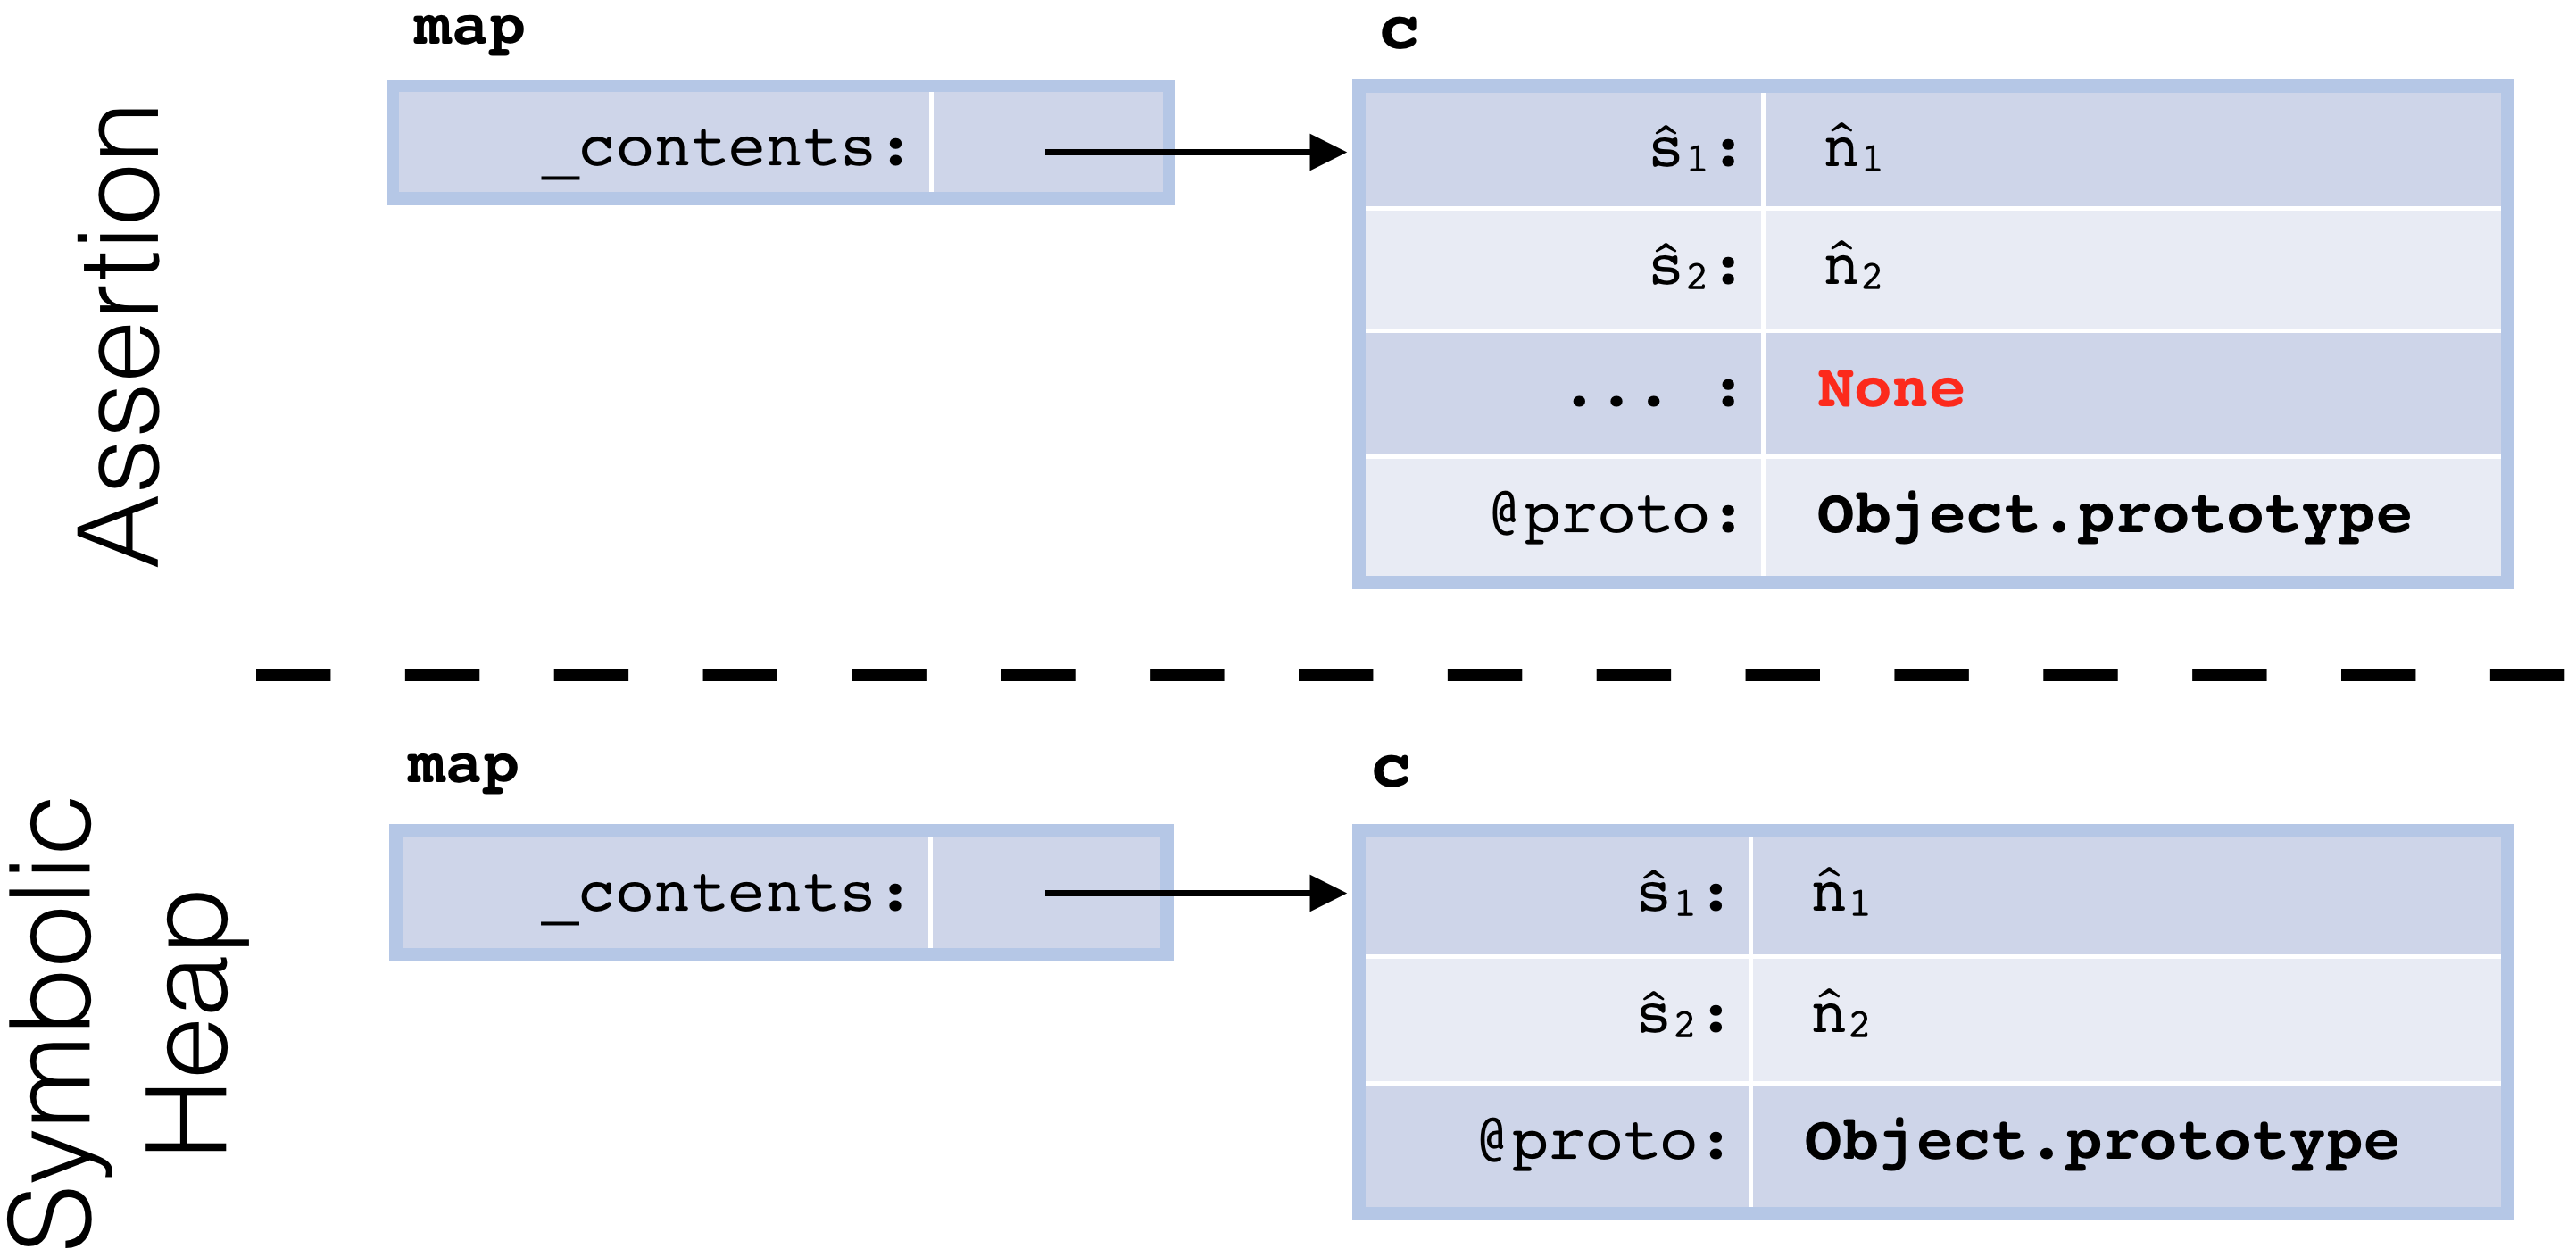
\includegraphics[width=\linewidth]{figures/symbvsass.png}

\vspace*{-0.7cm}
{\small $$
\text{\emph{Negative resource constraints: }} \{ \hat{s}_1, \hat{s}_2 \} \subseteq \{ \hat{s}_1, \hat{s}_2 \}
$$}
\vspace{-0.8cm}
\caption{Assertion vs. Symbolic Heap: {\small$\mathtt{Map(map, \{ (\hat{s}_1, \hat{n}_1), (\hat{s}_2, \hat{n}_2) \} )}$}}\label{fig:symb:state:versus:assertion}
\vspace{-0.5cm}
\end{figure}

\myparagraph{Example}
We illustrate the debugging of SL-specifications by appealing to the \jsinline|Map| example shown in Figure \ref{map:example}. In order to reason about a key-value map,
we define several predicates, whose definitions we show below.

\begin{Verbatim}[fontsize=\footnotesize,commandchars=\\\{\}]
Map (m, kvs) := 
  DataProp(m, "_contents", c) * JSObject(c) * 
    KVPairs(c, kvs) * first(kvs, keys) * emptyFields(c, keys)
\end{Verbatim}
 \begin{Verbatim}[fontsize=\footnotesize,commandchars=\\\{\}]
KVPairs (o, kvs) := 
  (kvs = \{ \}),
  (kvs = (k, v) -u- kvs') * ValidKey(k) * DataProp(o, k, v) * KVPairs(o, kvs')
\end{Verbatim}
\begin{Verbatim}[fontsize=\footnotesize,commandchars=\\\{\}]
ValidKey (k) := types(k : Str) * \textcolor{red}{(k <> "hasOwnProperty")}
\end{Verbatim}

The \jsinline|Map| predicate captures the resource corresponding to a map object. 
Concretely, it first states that the map object has the property \jsinline|_contents|, which points to a default JavaScript object \jsinline|c|, using the predicates \jsinline|DataProp| and \jsinline|JSObject|. 
\jsinline|DataProp(o, p, v)| captures the property \jsinline|p| of object \jsinline|o| and states that it has value \jsinline|v|, while abstracting over other associated JavaScript internals, whereas \jsinline|JSObject(o)| states that the object \jsinline|o| is an extensible object of class \jsinline|"Object"|, whose prototype is \jsinline|Object.prototype| (for more details, see~\cite{javert}). 
Next, using the \jsinline|KVPairs| predicate (explained shortly), it states that \jsinline|c| holds the key-value pairs \jsinline|kvs|. Finally, it states that \jsinline|c| has no other properties except the keys present in \jsinline|kvs|. For this, it first obtains the set of keys from the set of key-value pairs \jsinline|kvs| using the predicate \jsinline|first(kvs, keys)|, which states that the first projection of \jsinline|kvs| equals \jsinline|keys| (its definition is standard), and then uses the \jsinline|emptyFields| assertion to state that all other properties are absent from the object.

The \jsinline|KVPairs(o, kvs)| predicate talks about key-value pairs of an object \jsinline|o|. 
It is defined recursively on the structure of \jsinline|kvs| and it has two definitions, separated by a comma. 
We have that \jsinline|kvs| is either empty or that it contains at least one key-value pair \jsinline|(k, v)|.\footnote{We write {\small\texttt{-u-}} for set union and omit the brackets around singleton sets.} 
In the latter case, we state that the key \jsinline|k| must be valid, that the object \jsinline|o| has the property \jsinline|k| with value \jsinline|v|, and proceed recursively.
Note that the uniqueness of keys in \jsinline|kvs| is guaranteed by the \jsinline|DataProp| predicate of \jsinline|KVPairs| and the separating conjunction.

The \jsinline|ValidKey(k)| predicate captures the validity of a given key and holds \emph{iff} the corresponding JavaScript function \jsinline|validKey(k)| returns \jsinline|true|.
In the definition of \jsinline|ValidKey|, we highlight in red a potential source of errors on which we will focus shortly.

To give a better intuition of how the \jsinline|Map| predicate works, we show the full unfolding of {\small$\mathtt{Map(map, \{ (\hat{s}_1, \hat{n}_1), (\hat{s}_2, \hat{n}_2) \} )}$} in Figure \ref{fig:symb:state:versus:assertion}.
%a \emph{map object predicate}, \jsinline|Map|, 
%which uses the auxiliary predicate \jsinline|KVPairs|, capturing the resource of the key-value pairs in the map, 
%and the \jsinline|validKey(k)| predicate, which captures the validity of a key and holds if and only if the corresponding JavaScript function \jsinline|ValidKey(k)| returns \jsinline|true|\footnote{For the moment, we treat the $\mathtt{ValidKey}$ predicate as a black box.}.
%
%Intuitively, the \jsinline|Map(m, kvs)| predicate captures the resource 
%of a map object \jsinline|m| with key-value pairs \jsinline|kvs| (a set of string-number pairs, modelled as two-element lists).
%%\footnote{We model pairs as lists with two elements and, for clarity, use the pair notation.}). 
%For instance, the assertion $\mathtt{Map(map, \{ (\hat{s}_1, \hat{n}_1), (\hat{s}_2, \hat{n}_2) \} )}$ can be unfolded as illustrated in Figure~\ref{fig:symb:state:versus:assertion}. 
%Observe that the definition of \jsinline|Map| does not include the resource of a map prototype, as it is shared between all map objects, and therefore needs to be factored out.  
%
There, we can also see how the negative resource captured by the SL-assertion {\small$\mathtt{Map(map, \{ (\hat{s}_1, \hat{n}_1), (\hat{s}_2, \hat{n}_2) \} )}$}, namely the resource captured by {\small$\mathtt{emptyFields(c, first(kvs))}$}, disappears from the symbolic heap and is transformed into the negative resource constraint $\{ \hat{s}_1, \hat{s}_2 \} \subseteq \{ \hat{s}_1, \hat{s}_2 \}$, which states that all properties of the object \jsinline|c| in the symbolic heap (in our case, $\hat{s}_1$ and $\hat{s}_2$) must be in the set of properties of the corresponding \jsinline|emptyFields| assertion (in our case, {\small$\mathtt{first(\{ (\hat{s}_1, \hat{n}_1), (\hat{s}_2, \hat{n}_2) \}) = \{ \hat{s}_1, \hat{s}_2 \}}$}).
Such constraints are generated in item ${\bf e.}$ of the test generation algorithm presented in Figure \ref{fig:test:generation}. 

Below, we show the relevant parts of the specifications of \jsinline|get(k)| and \jsinline|put(k, v)|, for the case in which
 \jsinline|k| already exists in the map:

\noindent
\begin{minipage}{\linewidth}
\begin{displaymath} 
{\scriptsize
\hspace*{-0.2cm}
\begin{array}{c}
\left\{ {\begin{array}{c}
 \text{\texttt{Map(this, kvs -u- (k, v)) * ObjProtoF() *}} \\
 \text{\texttt{(this, "@proto") -> mp * MapProto(mp) * ...}}
\end{array}} \right\} \\
%
\text{\bfseries \texttt{get(k)}} \\[0.2mm]
%
\left\{ {\begin{array}{c}
 \text{\texttt{Precondition * (ret = v)}} 
\end{array}} \right\}
\end{array}
} 
\end{displaymath}
\end{minipage}
\quad
\begin{minipage}{\linewidth}
%
\begin{displaymath} 
{\scriptsize
\begin{array}{c}
\left\{ {\begin{array}{c}
 \text{\texttt{Map(this, kvs -u- (k, v')) * ObjProtoF() *}} \\
 \text{\texttt{(this, "@proto") -> mp * MapProto(mp) * ...}}
\end{array}} \right\} \\
%
\text{\bfseries \texttt{put(k, v)}} \\[0.2mm]
%
\left\{ {\begin{array}{c}
 \text{\texttt{Map(this, kvs -u- (k, v)) * ObjProtoF() *}} \\
 \text{\texttt{(this, "@proto") -> mp * MapProto(mp) * ...}}
\end{array}} \right\}
\end{array}
} 
\end{displaymath}
\end{minipage}

\vspace{10pt}
The predicate \jsinline|ObjProtoF()| describes the resource captured by the \jsinline|Object.prototype| object. 
In particular, it is needed because \texttt{get} uses the \texttt{hasOwnProperty} function, which is defined as a property of \jsinline|Object.prototype|. 
The predicate \jsinline|MapProto| specifies the resource of a valid map prototype: in particular, the map prototype needs to define the methods \jsinline|put|, \jsinline|get|, and \jsinline|validKey|. Finally, note that, given the definition of the \jsinline|Map| and \jsinline|KVPairs| predicates, both preconditions shown entail that \jsinline|k| is a valid key.

\begin{figure}[t!]
\centering
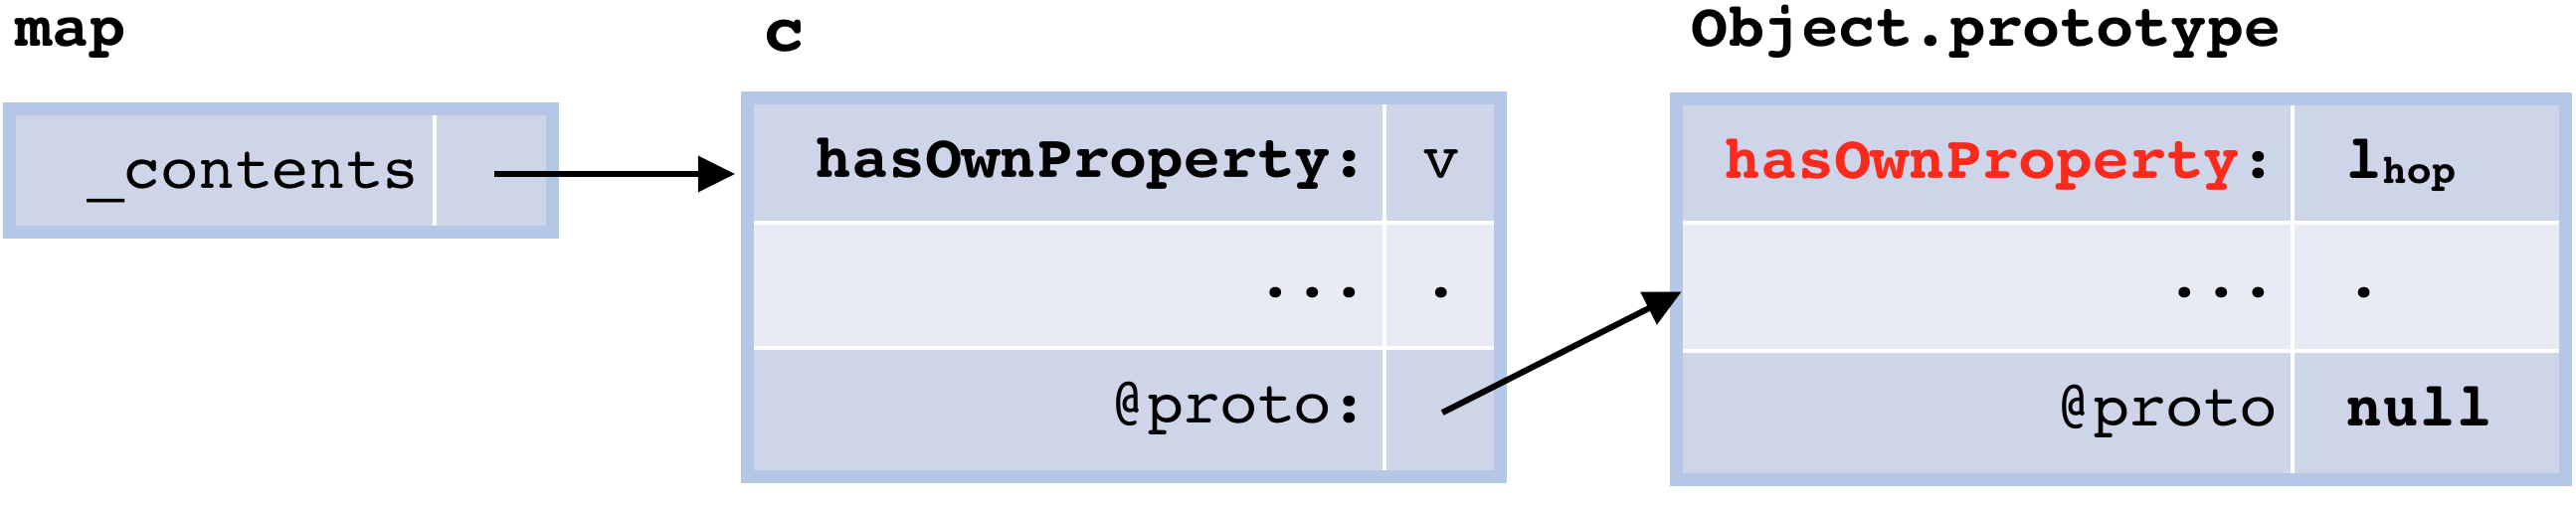
\includegraphics[width=\linewidth]{figures/heapfail.png}
\caption{Property shadowing: \jsinline|c.hasOwnProperty(...)| cannot reach \jsinline|Object.prototype|.} 
\label{fig:cexget}
\vspace{-0.5cm}
\end{figure}

Now, if we forgot to state the part of the $\mathtt{ValidKey(k)}$ predicate highlighted in red, that is, if we did not state that $\mathtt{k}$ needed to be different from \jsinline|"hasOwnProperty"|, the symbolic test generated for the specification of \jsinline|get| would fail for unfoldings of $\mathtt{KVPairs}$ of depth $\geq 1$, with the counter-model \jsinline|k = "hasOwnProperty"|. 
In that case, as illustrated in Figure~\ref{fig:cexget}, the \jsinline|"hasOwnProperty"| property of \jsinline|Object.prototype| would no longer be reachable by property lookup from \jsinline|c|, and
the execution of line~5 (\jsinline|if (c.hasOwnProperty(k))|) would raise an error, as it would attempt to call the \jsinline|"hasOwnProperty"| property of object \jsinline|c| as a function instead. 
Since this specification of $\mathtt{get(k)}$ requires normal termination, the jump to the error label in the compiled \jsil code will trigger the $\assert(\jfalse)$ of the generated symbolic test and the developer will be presented with the counter-model \jsinline|k = "hasOwnProperty"|.

\begin{center}
\polish{What else would we like to say here?}
\end{center}

%%
%% OLD THINGS

%\begin{figure}[t!]
%\centering
%{\scriptsize
%\begin{mathpar} 
%\inferrule[\textsc{New Existential}]
%     { 
%         \svar \in \existentials 
%         \quad
%         \svar \not\in \domain(\subst)
%     }
%     {\unification{\sexpr, \pc}{\svar}{\subst}{\existentials} = \optionsome{\subst[\svar \mapsto \sexpr]}}
%\quad
%\inferrule[\textsc{Matched Existential}]
%     { 
%         \subst(\svar) = \sexpr' 
%         \quad 
%         \pc \vdash \sexpr = \sexpr' 
%     }
%     {\unification{\sexpr, \pc}{\svar}{\subst}{\existentials} = \optionsome{\subst}}
%\quad
%\inferrule[\textsc{Existential - None}]
%     { 
%         \subst(\svar) = \sexpr' 
%         \quad 
%         \pc \vdash \sexpr \neq \sexpr' 
%     }
%     {\unificationfail{\sexpr, \pc}{\svar}{\subst}{\existentials} = \optionnone}
%\\
%\inferrule[\textsc{Grounded Expression}]
%     { 
%         \fv(\subst(\sexpr')) \cap \existentials = \emptyset
%         \quad 
%          \pc \vdash  \sexpr = \subst(\sexpr') 
%     }
%     {\unification{\sexpr, \pc}{\sexpr'}{\subst}{\existentials} = \optionsome{\subst}}
%\qquad
%\inferrule[\textsc{Grounded Expression - Fail}]
%     { 
%         \fv(\subst(\sexpr')) \cap \existentials = \emptyset
%         \quad 
%          \pc  \vdash  \sexpr \neq \subst(\sexpr') 
%     }
%     {\unification{\sexpr, \pc}{\sexpr'}{\subst}{\existentials} = \optionnone}
%%
%\\
%\inferrule[\textsc{Cell Assertion}]
%	{  
%	   \big(\loc = \symbeval{\lexpr_l}{\sstore} \ \vee \loc = \subst(\symbeval{\lexpr_l}{\sstore}) \big)
%	   \quad 
%	     \symbeval{\lexpr_p}{\sstore} = \sexprp'
%	   \quad
%	   \symbeval{\lexpr_v}{\sstore} = \sexprv' 
%	   \quad
%	    \sheap = \sheap_f \dunion ((l, \sexprp) \mapsto \sexprv) 
%	   \\
%	   \unification{\sexprp, \pc}{\sexprp'}{\subst}{\existentials} = \optionsome{\subst'} 
%	   \quad
%	   \unification{\sexprv, \pc}{\sexprv'}{\subst'}{\existentials} = \optionsome{\subst''} 
%	}{ \unification{\sheap, \sstore, \pc}{(\lexpr_l,\lexpr_p)\pointsto \lexpr_v}{\subst}{\existentials} = \optionsome{(\subst'', \sheap_f)}} 
%\\
%\inferrule[\textsc{Cell Assertion - Fail}]
%	{  
%	   \big(\loc = \symbeval{\lexpr_l}{\sstore} \ \vee \loc = \subst(\symbeval{\lexpr_l}{\sstore}) \big)
%	   \quad
%	     \symbeval{\lexpr_p}{\sstore} = \sexprp'
%	   \quad
%	   \symbeval{\lexpr_v}{\sstore} = \sexprv' 
%	   \quad
%	     \sheap = \sheap' \dunion  \big((l, \sexprp_i) \mapsto \sexprv_i\big)\mid_{i = 0}^n   
%  	   \\
%	    (l, -) \not\in \domain(\sheap') 
%	    \quad 
%	   \forall_{0 \leq i \leq n} \, \unification{\sexprp, \pc}{\sexprp'}{\subst}{\existentials} = \optionnone 
%	   \ \vee \
%	   \unification{\sexprv, \pc}{\sexprv'}{\subst'}{\existentials} = \optionnone
%	}{ \unification{\sheap, \sstore, \pc}{(\lexpr_l,\lexpr_p)\pointsto \lexpr_v}{\subst}{\existentials} = \optionnone} 
%\\
%\inferrule[\textsc{EmptyFields Assertion}]
%	{  
%	   \big(\loc = \symbeval{\lexpr_l}{\sstore} \ \vee \loc = \subst(\symbeval{\lexpr_l}{\sstore}) \big)
%	   \quad 
%	     \symbeval{\lexpr_d}{\sstore} = \sexprv' 
%	   \\\\
%	     \sheap = \sheap' \, \uplus \, \big((l, \sexprp_i) \mapsto \sexprv_i\big)\mid_{i = 0}^n   
%              \quad
%             (l, -) \not\in \domain(\sheap')
%	    \quad 
%	    \pc \vdash \big( \{ \sexprp_i \mid_{i = 0}^n   \} \subseteq \sexprv' \big)
%	}{ \unification{\sheap, \sstore, \pc}{\emptyfields{\lexpr_l}{\lexpr_d}}{\subst}{\existentials} = \optionsome{(\subst, \sheap)}} 
%\\
%\inferrule[\textsc{EmptyFields Assertion - Failing}]
%	{  
%	   \big(\loc = \symbeval{\lexpr_l}{\sstore} \ \vee \loc = \subst(\symbeval{\lexpr_l}{\sstore}) \big)
%	   \quad 
%	     \symbeval{\lexpr_d}{\sstore} = \sexprv' 
%	   \\\\
%	     \sheap = \sheap' \, \uplus \, \big((l, \sexprp_i) \mapsto \sexprv_i\big)\mid_{i = 0}^n   
%              \quad
%             (l, -) \not\in \domain(\sheap')
%	    \quad 
%	    \pc \vdash \big( \{ \sexprp_i \mid_{i = 0}^n   \} \not\subseteq \sexprv' \big)
%	}{ \unification{\sheap, \sstore, \pc}{\emptyfields{\lexpr_l}{\lexpr_d}}{\subst}{\existentials} = \optionnone} 
%\end{mathpar}
%\hrule
%\caption{Unification of spatial assertions:
% {\scriptsize$\unification{\sheap, \sstore, \pc}{\cell}{\subst}{\existentials} = (\subst', \sheap_f)$}\label{fig:unification}}}
%\end{figure}


%{\small 
%\begin{align}
%\sepmodels{P} = \left\{ (\iheap, \store) \mid \exists \senv \, . \,  \iheap, \store, \senv \satisfies P  \right\} 
%\\ 
%\smodels{\isheap, \sstore}{\pc} = \left\{ (\iheap, \store) \mid \exists \senv \, . \,  \senv \vdash \pc \ \wedge \
%    \iheap = \symbeval{\isheap}{\senv} \ \wedge \ \store = \symbeval{\sstore}{\senv}  \right\} 
%\end{align}} 



%
%\begin{figure}
%{\scriptsize
%\centering
%\begin{mathpar} 
%\inferrule[\textsc{Spatial Assertion}]
%	{  
%	   \unification{\sheap, \sstore, \pc}{(\lexpr_l,\lexpr_p)\pointsto \lexpr_v}{\subst} = \uyes{\sheap_f}
%	}{\cellunification{\sheap, \cell \lstcons \cells}{\sheap_q, \cells}{\sstore, \pc, \subst}} 
%\\
%\inferrule[\textsc{Successful Unification}]
%	{  
%	   
%	   \cellunificationiter{\sheap, \cells}{\hemp, []}{\sstore, \pc, \subst}
%	   \qquad 
%	   \pc \vdash \subst(\pfs')
%%	   \cells =  \cell \lstcons \cells'
%%	   \and
%%            \unification{\sheap, \sstore, \pc}{\cell}{\subst} = \uyes{\sheap_f}
%%            \\\\
%%            \unificationfull{\sheap_f, \sstore, \pc}{\cells', \pfs'}{\subst}
%	}{\unificationfull{\sheap, \sstore, \pc}{\cells, \pfs'}{\subst}} 
%\and 
%\inferrule[\textsc{Spatial Assertion}]
%	{  
%	   \cells = \cell \lstcons \cells'
%	   \and
%            \unification{\sheap, \sstore, \pc}{\cell}{\subst} = \uyes{\sheap_f}
%            \\\\
%            \unificationfullfail{\sheap_f, \sstore, \pc}{\cells', \pfs'}{\subst}{\pc'}
%	}{\unificationfullfail{\sheap, \sstore, \pc}{\cells, \pfs'}{\subst}{\pc'}} 
%\\
%\inferrule[\textsc{Pure Assertions}]
%	{  
%	   \pc \vdash \subst(\pfs')
%	}{\unificationfull{\hemp, \sstore, \pc}{\emptyset, \pfs'}{\subst}} 
%%
%\and
%%
%\qquad
%\inferrule[\textsc{Pure Assertions -  Fail}]
%	{  
%	      \pc \not\vdash \subst(\pfs')
%	}{\unificationfullfail{\sheap, \sstore, \pc}{\emptyset, \pfs'}{\subst}{\subst(\pfs')}} 
%\\
%%
%\inferrule[\textsc{Cell Assertion - Fail}]
%	{  
%	   \sfs = \cells \lstcons \cells
%	   \and
%            \unification{\sheap, \sstore, \pc}{\cell}{\subst} = \uno{\pc'}
%	}{\unificationfullfail{\sheap, \sstore, \pc}{\sfs, \pfs'}{\subst}{\pc'}} 
%%
%\and
%\inferrule[\textsc{Extra Resource -  Fail}]
%	{  
%	    \sheap \neq \hemp
%	}{\unificationfullfail{\sheap, \sstore, \pc}{\emptyset, \pfs'}{\subst}{\jtrue}} 
%%
%\end{mathpar}}
%\hrule



\section{OLD -- Evaluation}\label{sec:evaluation}
%!TEX root = ../main.tex

\subsection{Concrete interpreter evaluation}

Petar goes here

\subsection{Symbolic interpreter evaluation}

We validate \cosette as a JavaScript interpreter in paragraph~\ref{p1}, showcase its tractability by fully testing a library from node.js in paragraph~\ref{p2}, and demonstrate its symbolic bug-finding abilities with a real-world example in paragraph~\ref{p3}.

\myparagraph{Challenging JavaScript examples}

\cosette is able to verify JavaScript programs that use nontrivial parts of the JavaScript semantics, such as dynamic dispatch and property enumeration (via \jsinline{for-in} loops), in the symbolic world.

\subsubsection{Dynamic dispatch}
The following example demonstrates that \cosette is able to bring together complex symbolic string and mathematical reasoning with JavaScript's memory model.

\begin{lstjs}
var o = Object.create(null);

o.plusOne = function(x) { return x + 1 };
o.minusOne = function(x) { return x - 1 };

var s1 = symb_string(s1), s2 = symb_string(s2);
var n1 = symb_number(n1), n2 = symb_number(n2);

Assume(not (n1 = n2));

var total1 = o[s1](n1);
var total2 = o[s2](n2);

Assert(total1 = total2);
\end{lstjs}

In this example, we create an object \jsinline{o} that contains two functions, \jsinline{o.plusOne} and \jsinline{o.minusOne}, which respectively add and subtract $1$ from their argument.
We create two symbolic strings \jsinline{s1} and \jsinline{s2}, and two distinct symbolic numbers \jsinline{n1} and {n2}.
Then, we compute the result of applying function \jsinline{o[s1]} to \jsinline{n1}, and \jsinline{o[s2]} to \jsinline{n2}, stating with the \jsinline{Assert} statement that we want both these values to be equal.

According to the different values that the strings \jsinline{s1} and \jsinline{s2} take, quite different things can happen.
If \jsinline{s1} (or \jsinline{s2}) is not a valid property name of \jsinline{o}, the program will give a runtime error, because \jsinline{o[s1]} (or \jsinline{o[s2]}) evaluates to \jsinline{undefined}, which is not a function, and cannot be applied; when running the program with \cosette, we indeed get a concrete model for this failing case.

If both \jsinline{s1} and \jsinline{s2} are valid property names for \jsinline{o}, the program is always executed until its end.
In that case, \cosette is able to present us with a model for the final assertion to hold (for example, \jsinline{s1 = "minusOne", s2 = "plusOne", n1 = 0}, and \jsinline{n2 = -2}), as well as a model that invalidates the final assertion (for example, \jsinline{s1 = "minusOne", s2 = "minusOne", n1 = 0} and \jsinline{n2 = 1}).

This example demonstrates that \cosette has a fine understanding of the mechanics that underly the dynamic dispatch system in JavaScript, and is able to not only infer possible dynamic function names for a property function call to work, but is also able to relate the dynamic name to the function output.


\subsubsection{Property enumeration}
The following example demonstrates that \cosette is able to reason about the interplay of static and dynamic properties of JavaScript objects.

\begin{lstjs}

function nbProp(o) {
  var count = 0;
  for (var p in o) {
    count += 1;
  }
  return count;
}

var o = {a: 1, b: 2, c: 3};

var s1 = symb_string(s1);

o[s1] = 4;
var res = nbProp(o);
var expectedRes = 3;

Assert(res = expectedRes);
\end{lstjs}

In this example, we create a JavaScript object \jsinline{o} that has three properties \jsinline{a, b}, and \jsinline{c}.
Then, we create a symbolic string \jsinline{s1} and assign a value to the property of \jsinline{o} corresponding to {s1}.
Finally, we count the actual number of properties in \jsinline{o}.
There are two possible cases here: either \jsinline{s1} is equal to one of the concrete property names of \jsinline{o}, and the assignment actually overwrites the value associated with that property, or \jsinline{s1} is a fresh string and the assignment creates a new concrete property.

\cosette is able to reason about both cases, and finds a model for the assertion; either shadowing the property if \jsinline{expectedRes = 3}, giving a fresh string if \jsinline{expectedRes = 4}, or saying that the assertiong is unsatisfiable if \jsinline{expectedRes} is different from these two values.

This shows that \cosette is able to reason about the interplay between static and dynamic properties of JavaScript objects.
 
\myparagraph{Extensive testing of the BucketsJS library}

The BucketsJS library is a JavaScript data-structure library available on GitHub~\ref{buckets}.
It presents itself as \emph{fully tested}, and comes with a test suite that cover each of the data structures it exposes.
Using \cosette, we translated these concrete tests into symbolic tests that are shorter, easier to maintain, and have more extensive coverage.
We found that some code paths were never executed in the original tests, demonstrating that \cosette can be effectively used as a tool aiding test development.

\begin{table}[h]
{
\small
%\begin{center}
\begin{tabular}{lrrrr}
\toprule
File Name & JS Lines & JS Exec. lines & JSIL lines & Time (s)\\
\cmidrule{1-5}
\texttt{arrays.js} & 172 & 44 & 1251 & 0 \\
\texttt{bag.js} & 227 & 69 & 2041 & 0\\
\texttt{bstree.js} & 421 & 143 & 3819 & 0\\
\texttt{dictionary.js} & 210 & 57 & 1683 & 0\\
\texttt{heap.js} & 237 & 57 & 2059 & 0\\
\texttt{linkedlist.js} & 374 & 126 & 2447 & 0\\
\texttt{multidictionary.js} & 218 & 56 & 1871 & 0\\
\texttt{priorityqueue.js} & 162 & 26 & 1066 & 0\\
\texttt{queue.js} & 157 & 30 & 1095 & 0\\
\texttt{set.js} & 188 & 40 & 1528 & 0\\
\texttt{stack.js} & 153 & 23 & 941 & 0\\
\bottomrule
%\end{center}
\end{tabular}
}
\caption{Coverage analysis for the \texttt{buckets.js} library}
\end{table}
\FloatBarrier

for js lines: single + integrated
jsil lines: file itself, file + libraries

times: total time (racket) averaged over N times and solver time

% note: the - in \jsinline{queue-pri} doesn't have the same color as the rest (because it's a minus sign), find a nicer way to output this
\myparagraph{Debugging the \jsinline{queue-pri} library} 

The JavaScript \jsinline{queue-pri} library is a priority queue library available on GitHub~\ref{queue-pri}.
It provides a \jsinline{PriorityQueue} class; assuming object \jsinline{queue} is an instance of that class, the user can enqueue and dequeue objects with an integer priority value, by calling functions \jsinline{queue.enqueue(data, priority)} and \jsinline{queue.dequeue()}.
In this implementation, objects with smaller priority values are considered to have a higher priority and are dequeued first.
When enqueuing an object, the priority value is actually optional, and it will internally be replaced by \jsinline{null} if it isn't provided.
This means that the object will be dequeued last, after all the objects that have explicit priority values.
Using \cosette symbolic testing, we were able to find a bug in which the library does not respect the priority ordering of objects, and that is not covered by the test cases provided with the library.
When inserting an object with priority value $0$ (by calling \jsinline{queue.enqueue(obj, 0)}), the code actually replaces the priority by the \jsinline{null} value and places the object at the end of the queue.

\subsubsection{Symbolic test and countermodel}

We wrote the following symbolic example to test the code of the library.
We generate two symbolic strings \jsinline{s1} and \jsinline{s2}, which represent arbitrary data to be put in the queue, and two symbolic numbers \jsinline{x1} and \jsinline{x2} which represent the priority values.
Then, we enqueue first string \jsinline{s1} with priority \jsinline{x1}, then string \jsinline{s2} with priority \jsinline{x2}.
Finally, we dequeue the two strings into variables \jsinline{y1} and \jsinline{y2}, and we make sure that the ordering is consistent: either \jsinline{x1} $\leq$ \jsinline{x2}, in which case \jsinline{y1} $=$ \jsinline{s1} and \jsinline{y2} $=$ \jsinline{s2} (remember that lower priority number means higher priority), or \jsinline{x1} $>$ \jsinline{x2} and then \jsinline{y1} $=$ \jsinline{s2} and \jsinline{y2} $=$ \jsinline{s1}.

\begin{lstjs}
var x1 = symb_number(x1), x2 = symb_number(x2);
var s1 = symb_string(s1), s2 = symb_string(s2);

queue.enqueue(s1, x1);
queue.enqueue(s2, x2);

var y1 = queue.dequeue().data;
var y2 = queue.dequeue().data;

Assert(((x1 < x2) and (y1 = s1) and (y2 = s2)) 
    or ((x1 = x2) and (y1 = s1) and (y2 = s2))
    or ((x1 > x2) and (y1 = s2) and (y2 = s1)));
\end{lstjs}


However, when running this example with \cosette, we get the following countermodel, which invalidates the assertion: \jsinline{x1 = 1, x2 = 0, s1 = "!0!", s2 = "!1!"}.
When running the test with these concrete values, we indeed get \jsinline{y1 = "!0!" = s1}, and \jsinline{y2 = "!1!" = s2}, which contradicts the assertion.

\subsubsection{Origin of the bug and fix}

After inspecting the code, we found that the error comes from the \jsinline{queue.enqueue} function, specifically the following lines:

\begin{lstjs}
PriorityQueue.prototype = {
    ...,
    enqueue: function (data, pri) {
        var payload = {
            data: data,
            priority: pri || null
        };
        ...
    };
    ...
};
\end{lstjs}

When inserting an object with priority value \jsinline{pri = 0}, the \jsinline{pri || null} expression actually evaluates to \jsinline{null} instead of the expected \jsinline{0}, effectively disregarding the priority value.
This bug was not detected by the test suite provided with the library, because all of the tests use either \jsinline{null} or strictly positive priority values, but never \jsinline{0}.
We replaced the faulty line with an expression that correctly evaluates to 0 when \jsinline{pri} is equal to 0, and ran the symbolic test again; in this case, \cosette certified that the assertion always holds and that the fixed code is indeed correct, for all possible insertions of two objects with explicit priority values.

This examples shows that \cosette is capable to find bugs in real-world code, even in the presence of handwritten test cases, by generating symbolic examples that break the implicit assumptions made by the code, or by revealing corner cases that had not been considered.


\subsection{Spec-driven bugfinding}

José goes here

\bibliographystyle{ACM-Reference-Format}
\bibliography{biblio}

\end{document}
